    \begin{enumerate}[font=\bfseries]
        % ------------------------------------------ %
        %                      (2.1)                 %
        % ------------------------------------------ %
        \item[2.1]
        Let $\bold{x}^\prime = [5,1,3]$ and $\bold{y}^\prime = [-1,3,1]$.
        \begin{enumerate}
            \item Graph the two vectors.
            
            \begin{lstlisting}
x = [5,1,3]'; y = [-1,3,1]';
starts = zeros(2,3);  % Starts at the origin.
ends = [x'; y'];  % Ends at the point.

% quiver3 args are x,y,z,u,v,w. x,y,z are the start positions and u,v,w are the end positions.
a = quiver3(starts(:,1), starts(:,2), starts(:,3), ends(:,1), ends(:,2), ends(:,3));
axis equal
saveas(a, '.\applied-multivariate-statistics\solutions\chapter-2\sol2.1a.png', 'png')
            \end{lstlisting}

            \begin{figure}[H]
                \centering
                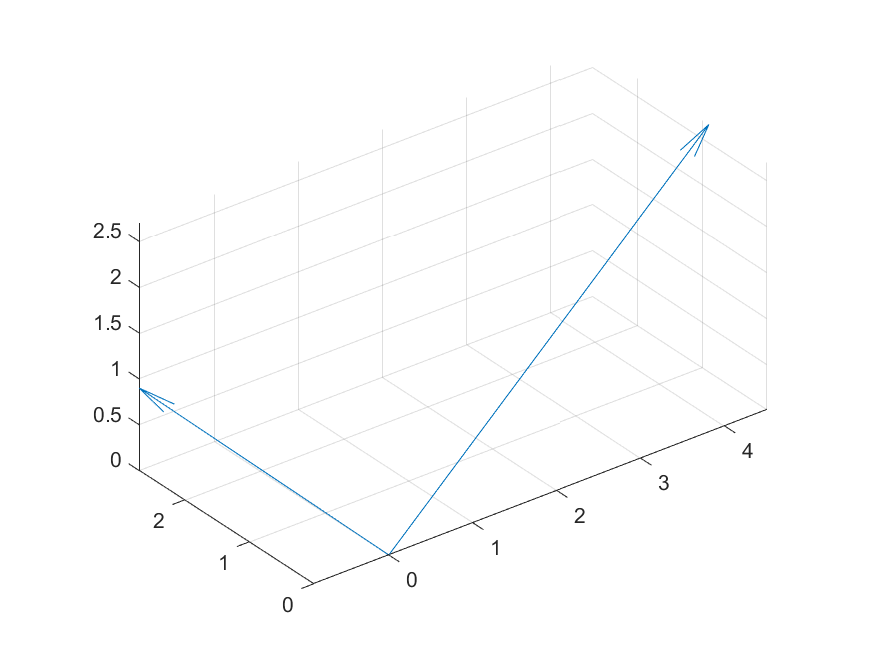
\includegraphics[scale=0.5]{./matlab/chapter-2/sol2.1a.png}
            \end{figure}
            

            \item Find (i) the length of $\bold{x}$, (ii) the angle between $\bold{x}$ and $\bold{y}$, and (iii) the projection of $\bold{y}$ onto $\bold{x}$.
            
\[
    \|\bold{x}\| = \sqrt{\bold{x}^\prime \bold{x}} = \sqrt{5^2 + 1^2 + 3^2} = 5.9161
\]

\[
    \bold{x} \cdot \bold{y} = \left\|\bold{x}\right\| \left\|\bold{y}\right\| \cos{\theta} 
    \Rightarrow \theta = \cos^{-1}{\left(\frac{\bold{x} \cdot \bold{y}}{\left\|\bold{x}\right\| \left\|\bold{y}\right\|}\right)} = \cos^{-1}{\left(\frac{1}{5.9161 \times 3.3166}\right)} = 87.0787 \degree
\]
MATLAB code \texttt{acosd((x'*y)/(norm(x)*norm(y)))} returns the angle in degrees.

\[
    \text{comp}_{\bold{x}}\bold{y} = \frac{\bold{x} \cdot \bold{y}}{\left\| \bold{x} \right\|}
\]

\[
    \text{proj}_{\bold{x}}\bold{y} = \text{comp}_{\bold{y}}\bold{x}\left(\frac{\bold{x}}{\left\|\bold{x}\right\|}\right) = \left(\frac{\bold{x} \cdot \bold{y}}{\left\| \bold{x} \right\|}\right) \left(\frac{\bold{x}}{\left\| \bold{x} \right\|}\right) = \left(\frac{\bold{x} \cdot \bold{y}}{\left\| \bold{x} \right\|^2}\right) \bold{x} = \left(\frac{1}{35}\right) \begin{bmatrix}
        5 \\
        1 \\
        3
    \end{bmatrix} =
    \begin{bmatrix}
        5/35 \\
        1/35 \\
        3/35
    \end{bmatrix}
\]

            \item Since $\bar{x} = 3$ and $\bar{y} = 1$, graph $[5-3, 1-3, 3-3] = [2, -2, 0]$ and $[-1-1, 3-1, 1-1] = [-2,2,0]$.
            
        \begin{lstlisting}
    starts = zeros(2,3);  % Starts at the origin.
    ends = [(x-mean(x))'; (y-mean(y))'];  % Ends at the point. Subtract the mean values.
    
    % quiver3 args are x,y,z,u,v,w. x,y,z are the start positions and u,v,w are
    % the end positions.
    b = quiver3(starts(:,1), starts(:,2), starts(:,3), ends(:,1), ends(:,2), ends(:,3));
    axis equal
    saveas(b, '.\applied-multivariate-statistics\solutions\chapter-2\sol2.1c.png', 'png')
        \end{lstlisting}

        \begin{figure}[H]
            \centering
            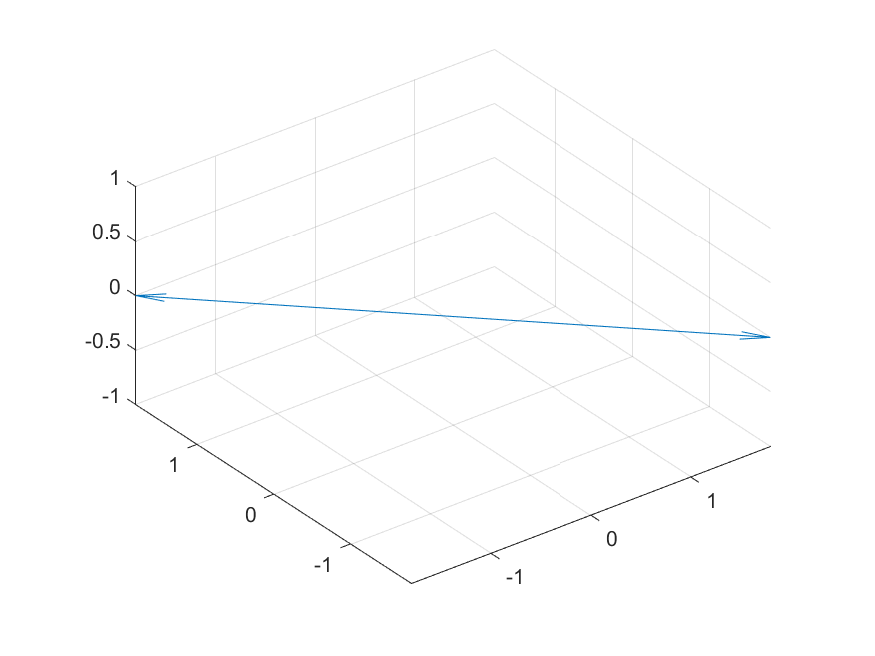
\includegraphics[scale=0.5]{./matlab/chapter-2/sol2.1c.png}
        \end{figure}

        After subtracting off the respective means from both $\bold{x}$ and $\bold{y}$ (centering), the results of both vectors exist on the same line through the origin, but point in different directions.
            
        \end{enumerate} 
        % ------------------------------------------ %
        %                      (2.2)                 %
        % ------------------------------------------ %
        \item[2.2]
        \[
            \bold{A} = \begin{bmatrix}
                -1 & 3 \\
                4 & 2  
              \end{bmatrix}\text{,}\hspace{0.2in}
            \bold{B} = \begin{bmatrix}
                4  & -3 \\
                1  & -2 \\
                -2 &  0
            \end{bmatrix}\text{,}\hspace{0.2in}\text{and}\hspace{0.2in}
            \bold{C} = \begin{bmatrix}
                5 \\
                -4 \\
                2
            \end{bmatrix}
        \]
        \begin{enumerate}
            \item $5\bold{A}$
            \[ 5\bold{A} =
            5 \begin{bmatrix}
              -1 & 3 \\
              4 & 2  
            \end{bmatrix} = 
            \begin{bmatrix}
                -5 & 15 \\
                20 & 10  
              \end{bmatrix}
            \]

            \item $\bold{BA}$
            

            \[
                \bold{BA} =
                \begin{bmatrix}
                    4  & -3 \\
                    1  & -2 \\
                    -2 &  0
                \end{bmatrix}
                \begin{bmatrix}
                    -1 & 3 \\
                    4 & 2  
                  \end{bmatrix} =
                  \begin{bmatrix}
                    -16  & 6 \\
                    -9 & -1 \\
                    2 &  -6
                \end{bmatrix}
            \]

            \item $\bold{A}^\prime \bold{B}^\prime$
            

            \[
                \bold{A}^\prime \bold{B}^\prime =
                \begin{bmatrix}
                    -1 & 4 \\
                    3 & 2
                \end{bmatrix}
                \begin{bmatrix}
                    4 & 1 & -2 \\
                    -3 & -2 & 0
                \end{bmatrix} = 
                \begin{bmatrix}
                    -16 & -9 & 2 \\
                    6 & -1 & -6
                \end{bmatrix}
            \]


            \item $\bold{C}^\prime \bold{B}$
            

            \[
                \bold{C}^\prime \bold{B} =
                \begin{bmatrix}
                    5 & -4 & 2
                \end{bmatrix}
                \begin{bmatrix}
                    4  & -3 \\
                    1  & -2 \\
                    -2 &  0
                \end{bmatrix} =
                \begin{bmatrix}
                    12  & -7
                \end{bmatrix}
            \]


            \item Is $\bold{AB}$ defined?
            

            No, $\bold{A}$ is a $2 \times 2$ matrix and $\bold{B}$ is a $3 \times 2$ matrix, the number of columns in $\bold{A} = 2$ is not the same as the number of rows in $\bold{B} = 3$, so the two matrices are not conformable.


        \end{enumerate}
        % ------------------------------------------ %
        %                      (2.3)                 %
        % ------------------------------------------ %
        \item[2.3] 
        Verify the following properties of transpose when
        \[
            \bold{A} = \begin{bmatrix}
                2 & 1 \\
                1 & 3
            \end{bmatrix}\text{,}\hspace{0.2in}
            \bold{B} = \begin{bmatrix}
                1 & 4 & 2 \\
                5 & 0 & 3
            \end{bmatrix}\text{,}\hspace{0.2in}\text{and}\hspace{0.2in}
            \bold{C} = \begin{bmatrix}
                1 & 4 \\
                3 & 2
            \end{bmatrix},
        \]
        \begin{enumerate}
            \item ${\left(\bold{A}^\prime\right)}^\prime = \bold{A}$
            

            \[
                {\left(\bold{A}^\prime\right)}^\prime = 
                {\left(
                    \begin{bmatrix}
                        2 & 1 \\
                        1 & 3
                    \end{bmatrix}^\prime
                    \right)}^\prime =
                {\left(
                    \begin{bmatrix}
                        2 & 1 \\
                        1 & 3
                    \end{bmatrix}
                    \right)}^\prime = 
                    \begin{bmatrix}
                        2 & 1 \\
                        1 & 3
                    \end{bmatrix} =
                    \bold{A}
            \]

            Matrix $\bold{A}$ is symmetric since $\bold{A} = \bold{A}^\prime$.


            \item ${\left(\bold{C}^\prime\right)}^{-1} = {\left(\bold{C}^{-1}\right)}^\prime$
            

            \[
                {\left(\bold{C}^\prime\right)}^{-1} = 
                {\left(
                    {\begin{bmatrix}
                        1 & 4 \\
                        3 & 2
                    \end{bmatrix}}^\prime\right)
                }^{-1} =
                {\begin{bmatrix}
                        1 & 3 \\
                        4 & 2
                \end{bmatrix}}^{-1} =
                \frac{1}{2-12}
                \begin{bmatrix}
                    2 & -3 \\
                    -4 & 1
                \end{bmatrix} =
                \begin{bmatrix}
                    -2/10 & 3/10 \\
                    4/10 & -1/10
                \end{bmatrix}
            \]

            \[
                {\left(\bold{C}^{-1}\right)}^\prime =
                {\left(
                    {\begin{bmatrix}
                        1 & 4 \\
                        3 & 2
                    \end{bmatrix}}^{-1}\right)
                }^\prime =
                {\frac{1}{2-12}
                {\begin{bmatrix}
                    2 & -4 \\
                    -3 & 1
                \end{bmatrix}}
                }^\prime =
                \begin{bmatrix}
                    -2/10 & 3/10 \\
                    4/10 & -1/10
                \end{bmatrix}
            \]
            So ${\left(\bold{C}^\prime\right)}^{-1} = {\left(\bold{C}^{-1}\right)}^\prime$.

            \item ${\left(\bold{AB}\right)}^\prime = \bold{B}^\prime \bold{A}^\prime$
            
            \[
                {\left(\bold{AB}\right)}^\prime = 
                {\left(
                    \begin{bmatrix}
                        2 & 1 \\
                        1 & 3
                    \end{bmatrix}
                    \begin{bmatrix}
                        1 & 4 & 2 \\
                        5 & 0 & 3
                    \end{bmatrix}
                \right)}^\prime =
                {\begin{bmatrix}
                    7 & 8 & 7 \\
                    16 & 4 & 11
                \end{bmatrix}}^\prime =
                \begin{bmatrix}
                    7 & 16 \\
                    8 & 4 \\
                    7 & 11
                \end{bmatrix}
            \]

            \[
                \bold{B}^\prime \bold{A}^\prime =
                {\begin{bmatrix}
                    1 & 4 & 2 \\
                    5 & 0 & 3
                \end{bmatrix}}^\prime
                {\begin{bmatrix}
                    2 & 1 \\
                    1 & 3
                \end{bmatrix}}^\prime =
                \begin{bmatrix}
                    1 & 5 \\
                    4 & 0 \\
                    2 & 3
                \end{bmatrix}
                \begin{bmatrix}
                    2 & 1 \\
                    1 & 3
                \end{bmatrix} =
                \begin{bmatrix}
                    7 & 16 \\
                    8 & 4 \\
                    7 & 11
                \end{bmatrix}
            \]

            So ${\left(\bold{AB}\right)}^\prime = \bold{B}^\prime \bold{A}^\prime$.

            \item For general $\underset{\left(m\times k\right)}{\bold{A}}$ and $\underset{\left(k\times l\right)}{\bold{B}}$, ${\left(\bold{AB}\right)}^\prime = \bold{B}^\prime\bold{A}^\prime$.
            
            \[
                {\left(\bold{AB}\right)}^\prime =
                {\left(
                \begin{bmatrix}
                    a_{11} & \dots & a_{1k} \\
                    \vdots & \ddots & \vdots \\
                    a_{m1} & \dots & a_{mk}
                \end{bmatrix}
                \begin{bmatrix}
                    b_{11} & \dots & b_{1\ell} \\
                    \vdots & \ddots & \vdots \\
                    b_{k1} & \dots & b_{k\ell}
                \end{bmatrix}
                \right)}^\prime = 
                {\left(
                \begin{bmatrix}
                    \sum_{i=1}^k{a_{1i}b_{i1}} & \dots & \sum_{i=1}^k{a_{1i}b_{i\ell}} \\
                    \vdots & \ddots & \vdots \\
                    \sum_{i=1}^k{a_{mi}b_{i1}} & \dots & \sum_{i=1}^k{a_{mi}b_{i\ell}}
                \end{bmatrix}
                \right)}^\prime = 
            \]
            \[
                = \begin{bmatrix}
                    \sum_{i=1}^k{a_{1i}b_{i1}} & \dots & \sum_{i=1}^k{a_{mi}b_{i1}} \\
                    \vdots & \ddots & \vdots \\
                    \sum_{i=1}^k{a_{1i}b_{i\ell}} & \dots & \sum_{i=1}^k{a_{mi}b_{i\ell}}
                \end{bmatrix}
            \]

            \[
                \bold{B}^\prime \bold{A}^\prime = 
                \begin{bmatrix}
                    b_{11} & \dots & b_{1\ell} \\
                    \vdots & \ddots & \vdots \\
                    b_{k1} & \dots & b_{k\ell}
                \end{bmatrix}^\prime
                \begin{bmatrix}
                    a_{11} & \dots & a_{1k} \\
                    \vdots & \ddots & \vdots \\
                    a_{m1} & \dots & a_{mk}
                \end{bmatrix}^\prime =
                \begin{bmatrix}
                    b_{11} & \dots & b_{k1} \\
                    \vdots & \ddots & \vdots \\
                    b_{1\ell} & \dots & b_{k\ell}
                \end{bmatrix}
                \begin{bmatrix}
                    a_{11} & \dots & a_{m1} \\
                    \vdots & \ddots & \vdots \\
                    a_{1k} & \dots & a_{mk}
                \end{bmatrix} =
            \]

            \[
                = \begin{bmatrix}
                    \sum_{i=1}^k{b_{i1}a_{1i}} & \dots & \sum_{i=1}^k{b_{i1}a_{mi}} \\
                    \vdots & \ddots & \vdots \\
                    \sum_{i=1}^k{b_{i\ell}a_{1i}} & \dots & \sum_{i=1}^k{b_{i\ell}a_{mi}}
                \end{bmatrix} = \begin{bmatrix}
                    \sum_{i=1}^k{a_{1i}b_{i1}} & \dots & \sum_{i=1}^k{a_{mi}b_{i1}} \\
                    \vdots & \ddots & \vdots \\
                    \sum_{i=1}^k{a_{1i}b_{i\ell}} & \dots & \sum_{i=1}^k{a_{mi}b_{i\ell}}
                \end{bmatrix}
            \]
        \end{enumerate}
        So ${\left(\bold{AB}\right)}^\prime = \bold{B}^\prime\bold{A}^\prime$.
        % ------------------------------------------ %
        %                      (2.4)                 %
        % ------------------------------------------ %
        \item[2.4] When $\bold{A}^{-1}$ and $\bold{B}^{-1}$ exist, prove each of the following.
        \begin{enumerate}
            \item ${\left(\bold{A}^\prime\right)}^{-1} = {\left(\bold{A}^{-1}\right)}^\prime$
            
            \[
                {\left(\bold{A}^{-1}\right)}^\prime = {\left(\bold{A}^{-1}\right)}^\prime \bold{I} = {\left(\bold{A}^{-1}\right)}^\prime\bold{A}^\prime{\left(\bold{A}^\prime\right)}^{-1} =
                {\left(\bold{A}\bold{A}^{-1}\right)}^\prime{\left(\bold{A}^\prime\right)}^{-1} = \bold{I}{\left(\bold{A}^\prime\right)}^{-1} = {\left(\bold{A}^\prime\right)}^{-1}
            \]

            \item ${\left(\bold{A}\bold{B}\right)}^{-1} = \bold{B}^{-1} \bold{A}^{-1}$
            
            If we define $\bold{C} = \bold{A}\bold{B}$ and $\bold{D} = \bold{B}^{-1}\bold{A}^{-1}$, and if \textbf{Def 2A.27} is satisifed ($\bold{C}\bold{D} = \bold{D}\bold{C} = \bold{I}$), then $\bold{D}$ is the inverse of $\bold{C}$.
            \[
                \bold{C}\bold{D} = \left(\bold{A}\bold{B}\right)\left({\bold{B}}^{-1}{\bold{A}}^{-1}\right) = \bold{A}\left(\bold{B}{\bold{B}}^{-1}\right){\bold{A}}^{-1} = \bold{A}\bold{I}{\bold{A}}^{-1} = \bold{A}{\bold{A}}^{-1} = \bold{I}
            \]

            \[
                \bold{D}\bold{C} = \left({\bold{B}}^{-1}{\bold{A}}^{-1}\right)\left(\bold{A}\bold{B}\right) = \bold{B}\left(\bold{A}{\bold{A}}^{-1}\right){\bold{B}}^{-1} = \bold{B}\bold{I}{\bold{B}}^{-1} = \bold{B}{\bold{B}}^{-1} = \bold{I}
            \]
            Now, \textbf{Def 2A.27} is satisifed ($\bold{C}\bold{D} = \bold{D}\bold{C} = \bold{I}$), so the inverse of $\bold{A}\bold{B}$ is $\bold{B}^{-1}\bold{A}^{-1}$. That is, ${\left(\bold{A}\bold{B}\right)}^{-1} = \bold{B}^{-1} \bold{A}^{-1}$.
            \newline
            \newline
            Hint: Part a can be proven noting that $\bold{A}\bold{A}^{-1} = \bold{I}$, $\bold{I} = \bold{I}^\prime$, and ${\left(\bold{A}\bold{A}^{-1}\right)}^\prime = {\left(\bold{A}^{-1}\right)}^\prime \bold{A}^\prime$. Part b follows from $\left(\bold{B}^{-1}\bold{A}^{-1}\right) \bold{AB} = \bold{B}^{-1}\left(\bold{A}^{-1}\bold{A}\right)\bold{B} = \bold{B}^{-1}\bold{B} = \bold{I}$.
        \end{enumerate}
        % ------------------------------------------ %
        %                      (2.5)                 %
        % ------------------------------------------ %
        \item[2.5] Check that
        
        \[
            \bold{Q} = \begin{bmatrix}
                \frac{5}{13} & \frac{12}{13} \\
                \frac{-12}{13} & \frac{5}{13}
            \end{bmatrix}
        \]
        is an orthogonal matrix.
        \newline
        \newline
        If the conditions of \textbf{Result 2A.13}, ($\bold{A}\bold{A}^\prime = \bold{A}^\prime \bold{A} = \bold{I}$) are true, then we have an orthogonal matrix.
        \[
            \bold{Q}^\prime \bold{Q} = 
            \begin{bmatrix}
                \frac{5}{13} & \frac{-12}{13} \\
                \frac{12}{13} & \frac{5}{13}
            \end{bmatrix}
            \begin{bmatrix}
                \frac{5}{13} & \frac{12}{13} \\
                \frac{-12}{13} & \frac{5}{13}
            \end{bmatrix} =
            \begin{bmatrix}
                \frac{25}{169} + \frac{144}{169} & \frac{60}{169} - \frac{60}{169} \\
                \frac{60}{169} - \frac{60}{169} & \frac{144}{169} + \frac{25}{169}
            \end{bmatrix} =
            \begin{bmatrix}
                \frac{169}{169} & \frac{0}{169} \\
                \frac{0}{169} & \frac{169}{169}
            \end{bmatrix} =
            \bold{I}
        \]

        \[
            \bold{Q} \bold{Q}^\prime = 
            \begin{bmatrix}
                \frac{5}{13} & \frac{12}{13} \\
                \frac{-12}{13} & \frac{5}{13}
            \end{bmatrix}
            \begin{bmatrix}
                \frac{5}{13} & \frac{-12}{13} \\
                \frac{12}{13} & \frac{5}{13}
            \end{bmatrix} =
            \begin{bmatrix}
                \frac{25}{169} + \frac{144}{169} & -\frac{60}{169} + \frac{60}{169} \\
                -\frac{60}{169} + \frac{60}{169} & \frac{144}{169} + \frac{25}{169}
            \end{bmatrix} =
            \begin{bmatrix}
                \frac{169}{169} & \frac{0}{169} \\
                \frac{0}{169} & \frac{169}{169}
            \end{bmatrix} =
            \bold{I}
        \]
        Because $\bold{Q}\bold{Q}^\prime = \bold{Q}^\prime \bold{Q} = \bold{I}$, $\bold{Q}$ is an orthofonal matrix.
        % ------------------------------------------ %
        %                      (2.6)                 %
        % ------------------------------------------ %
        \item[2.6] Let
        \[
            \bold{A} = \begin{bmatrix}
                9 & -2 \\
                -2 & 6
            \end{bmatrix}
        \]
        \begin{enumerate}
            \item Is $\bold{A}$ symmetric?
            \par
            Yes, $\bold{A}^{\prime} = \bold{A}$, so $\bold{A}$ is symmetric.
            \item Show that $\bold{A}$ is positive definite.
            
            \[
                0 = \left|\bold{A} - \lambda \bold{I}\right| =
                \left|\begin{matrix}
                    9-\lambda & -2 \\
                    -2 & 6-\lambda
                \end{matrix}
                \right| = \left(9 - \lambda\right)\left(6 - \lambda\right) - 4 = \lambda^2 - 15\lambda + 54 - 4 = \left(\lambda - 5\right)\left(\lambda - 10\right)
            \]
        The two eigenvalues of 5 and 10 are both positive, so from what's in \textbf{2.3} on page 63, $\bold{A}$ is positive definite.
        \end{enumerate}
        % ------------------------------------------ %
        %                      (2.7)                 %
        % ------------------------------------------ %
        \item[2.7] Let $\bold{A}$ be as given in Exercise 2.6.
        \begin{enumerate}
            \item Determine the eigenvalues and eigenvectors of $\bold{A}$.
            \par
            From problem 2.7, the eigenvalues are 5 and 10.To get the eigenvectors,
            \newline
            $\underline{\lambda_1 = 5}$:
            \[
                \bold{A}\bold{x}_1 = \lambda_1 \bold{x}_1
                \begin{bmatrix}
                    9 & -2 \\
                    -2 & 6
                \end{bmatrix} \Rightarrow
                \begin{bmatrix}
                    9 & -2 \\
                    -2 & 6
                \end{bmatrix}
                \begin{bmatrix}
                    x_1 \\
                    x_2
                \end{bmatrix} = 
                5\begin{bmatrix}
                    x_1 \\
                    x_2
                \end{bmatrix}
            \]
            \[
                9x_1 - 2x_2 = 5x_1 \Rightarrow 4x_1 = 2x_2 \Rightarrow 2x_1 = x_2
            \]
            and
            \[
                -2x_1 + 6x_2 = 5x_1 \Rightarrow x_2 = 2x_1
            \]
            So $\bold{x}_2 = \begin{bmatrix}
                1 \\
                2
            \end{bmatrix}$ and normalizing, $\bold{e}_1 = \begin{bmatrix}
                1/\sqrt{5} \\
                2/\sqrt{5}
            \end{bmatrix}$.
            \newline
            $\underline{\lambda_2 = 10}$:
            \[
                \bold{A}\bold{x}_2 = \lambda_2 \bold{x}_2
                \begin{bmatrix}
                    9 & -2 \\
                    -2 & 6
                \end{bmatrix} \Rightarrow
                \begin{bmatrix}
                    9 & -2 \\
                    -2 & 6
                \end{bmatrix}
                \begin{bmatrix}
                    x_1 \\
                    x_2
                \end{bmatrix} = 
                10\begin{bmatrix}
                    x_1 \\
                    x_2
                \end{bmatrix}
            \]
            \[
                9x_1 - 2x_2 = 10x_1 \Rightarrow x_1 = -2x_2
            \]
            and
            \[
                -2x_1 + 6x_2 = 10x_1 \Rightarrow 12x_1 = -6x_2 \Rightarrow x_1 = -2x_2
            \]
            So $\bold{x}_2 = \begin{bmatrix}
                -2 \\
                1
            \end{bmatrix}$ and normalizing, $\bold{e}_2 = \begin{bmatrix}
                -2/\sqrt{5} \\
                1/\sqrt{5}
            \end{bmatrix}$.
            \item Write the spectral decomposition of $\bold{A}$.
            \par
            The spectral decomposition would be,
            \[
                \bold{A} = \sum_{k=1}^2{\lambda_k\bold{e}_k\bold{e}_k^\prime} = 
                5 \begin{bmatrix}
                    1/\sqrt{5} \\
                    2/\sqrt{5}
                \end{bmatrix}
                \begin{bmatrix}
                    1/\sqrt{5} \\
                    2/\sqrt{5}
                \end{bmatrix}^\prime + 
                10 \begin{bmatrix}
                    -2/\sqrt{5} \\
                    1/\sqrt{5}
                \end{bmatrix}
                \begin{bmatrix}
                    -2/\sqrt{5} \\
                    1/\sqrt{5}
                \end{bmatrix}^\prime = 
            \]
            \[
                =
                5 \begin{bmatrix}
                    1/5 & 2/5 \\
                    2/5 & 4/5
                \end{bmatrix} + 
                10 \begin{bmatrix}
                    4/5 & -2/5 \\
                    -2/5 & 1/5
                \end{bmatrix}
                =
                \begin{bmatrix}
                    1 & 2 \\
                    2 & 4
                \end{bmatrix} + 
                \begin{bmatrix}
                    8 & -4 \\
                    -4 & 2
                \end{bmatrix} =
                \begin{bmatrix}
                    9 & -2 \\
                    -2 & 6
                \end{bmatrix}
            \]
            \item Find $\bold{A}^{-1}$.
            \par
            Using the spectral decomposition for the inverse in \textbf{(2-21)} on page 66,
            \[
                \bold{A}^{-1} = 
                {\left(\bold{P}
                \bold{\Lambda}
                \bold{P}^\prime\right)}^{-1} = 
                {\left(\begin{bmatrix}
                    \bold{e}_1 & \bold{e}_2
                \end{bmatrix}
                \bold{\Lambda}
                \begin{bmatrix}
                    \bold{e}_1 & \bold{e}_2
                \end{bmatrix}^\prime\right)}^{-1} = 
                \begin{bmatrix}
                    \bold{e}_1 & \bold{e}_2
                \end{bmatrix}
                {\bold{\Lambda}}^{-1}
                \begin{bmatrix}
                    \bold{e}_1 & \bold{e}_2
                \end{bmatrix}^\prime =
            \]
            \[
                =
                \begin{bmatrix}
                    1/\sqrt{5} & -2/\sqrt{5} \\
                    2/\sqrt{5} & 1/\sqrt{5}
                \end{bmatrix}
                \begin{bmatrix}
                    1/5 & 0 \\
                    0 & 1/10
                \end{bmatrix}
                \begin{bmatrix}
                    1/\sqrt{5} & 2/\sqrt{5} \\
                    -2/\sqrt{5} & 1/\sqrt{5}
                \end{bmatrix} =
                \frac{1}{5}
                \begin{bmatrix}
                    1/5 & -2/10 \\
                    2/5 & 1/10
                \end{bmatrix}
                \begin{bmatrix}
                    1 & 2 \\
                    -2 & 1
                \end{bmatrix} =
            \]
            \[
                =
                \frac{1}{5}
                \begin{bmatrix}
                    30/50 & 10/50 \\
                    10/50 & 45/50
                \end{bmatrix}
                =
                \frac{1}{50}
                \begin{bmatrix}
                    6 & 2 \\
                    2 & 9
                \end{bmatrix}
            \]

            By direct computation,
            \[
                \bold{A}^{-1} = 
                \begin{bmatrix}
                    9 & -2 \\
                    -2 & 6
                \end{bmatrix}^{-1} = 
                \frac{1}{54-4}
                \begin{bmatrix}
                    6 & 2 \\
                    2 & 9
                \end{bmatrix} =
                \frac{1}{50}
                \begin{bmatrix}
                    6 & 2 \\
                    2 & 9
                \end{bmatrix}
            \]
            \item Find the eigenvalues and eigenvectors of $\bold{A}^{-1}$.
            \par
            Using \textbf{2-21} on page 66 again, the eigenvalues of $\bold{A}^{-1}$ are the reciprocal of the eigenvalues of $\bold{A}$ and the eigenvectors are the same as those for $\bold{A}$.
            \[
                \bold{\Lambda}^{-1}
                =
                \begin{bmatrix}
                    1/5 & 0 \\
                    0 & 1/10
                \end{bmatrix}
            \]
            \[
                \bold{P} =
                \begin{bmatrix}
                    \bold{e}_1 & \bold{e}_2
                \end{bmatrix} =
                \begin{bmatrix}
                    1/\sqrt{5} & -2/\sqrt{5} \\
                    2/\sqrt{5} & 1/\sqrt{5}
                \end{bmatrix}
            \]
            If we did it by-hand, setting $\bold{B} = \bold{A}^{-1}$,
            \[
                0 = \left|\bold{B} - \lambda\bold{I}\right|
                =
                \frac{1}{50}
                \left|
                \begin{matrix}
                    6 - \lambda & 2 \\
                    2 & 9 - \lambda
                \end{matrix}
                \right| = 
                \frac{1}{50} \left[\left(6 - \lambda\right)\left(9 - \lambda\right) - 54 + 4\right] =
                \frac{1}{50} \left[\left(6 - \lambda\right)\left(9 - \lambda\right) - 50\right] =
            \]
            \[
                \frac{1}{50} \left(\lambda^2 - 15\lambda + 50\right) =
                \left(\lambda - \frac{5}{50}\right)\left(\lambda - \frac{10}{50}\right) =
                \left(\lambda - \frac{1}{10}\right)\left(\lambda - \frac{1}{5}\right)
            \]
            These eigenvalues are the same as the reciprocal of the eigenvalues for $\bold{A}$.
        \end{enumerate}
        % ------------------------------------------ %
        %                      (2.8)                 %
        % ------------------------------------------ %
        \item[2.8] Given the matrix
        \[
            \bold{A} = \begin{bmatrix}
                1 & 2 \\
                2 & -2
            \end{bmatrix}
        \]
        find the eigenvalues $\lambda_1$ and $\lambda_2$ and the associated eigenvectors $\bold{e}_1$ and $\bold{e}_2$. Determine the spectral decomposition \textbf{(2-16)} of $\bold{A}$.
        \par
        \[
            0 = \left|\bold{A} - \lambda\bold{I}\right|
            =
            \left|
            \begin{matrix}
                1 - \lambda & 2 \\
                2 & -2 - \lambda
            \end{matrix}
            \right|
            =
            \left(1 - \lambda\right)\left(-2-\lambda\right) - 4
            =
            -2 + 2\lambda - \lambda + \lambda^2 - 4
            =
        \]
        \[
            = \lambda^2 + \lambda - 6
            = \left(\lambda + 3 \right)\left(\lambda - 2\right)
        \]
        The eigenvalues are -3 and 2.
        \newline
        $\underline{\lambda_1 = -3}$:
        \[
            \bold{A}\bold{x}_1 = \lambda\bold{x}_1
            \Rightarrow
            \bold{A} = \begin{bmatrix}
                1 & 2 \\
                2 & -2
            \end{bmatrix}
            \begin{bmatrix}
                x_1 \\
                x_2
            \end{bmatrix}
            =
            \begin{bmatrix}
                -3x_1 \\
                -3x_2
            \end{bmatrix}
        \]
        \[
            x_1 + 2x_2 = -3x_1
            \Rightarrow
            -4x_1 = 2x_2
            \Rightarrow
            -2x_1 = x_2
        \]
        and
        \[
            2x_1 - 2x_2 = -3x_1
            \Rightarrow
            2x_1 = -x_2
            \Rightarrow
            -2x_1 = x_2
        \]
        So $\bold{x}_1 = \begin{bmatrix}
            1 \\
            -2
        \end{bmatrix}$ and normalizing $\bold{e}_1 = \begin{bmatrix}
            1/\sqrt{5} \\
            -2/\sqrt{5}
        \end{bmatrix}$.
        \newline
        $\underline{\lambda_2 = 2}$:
        \[
            \bold{A}\bold{x}_2 = \lambda\bold{x}_2
            \Rightarrow
            \bold{A} = \begin{bmatrix}
                1 & 2 \\
                2 & -2
            \end{bmatrix}
            \begin{bmatrix}
                x_1 \\
                x_2
            \end{bmatrix}
            =
            \begin{bmatrix}
                2x_1 \\
                2x_2
            \end{bmatrix}
        \]
        \[
            x_1 + 2x_2 = 2x_1
            \Rightarrow
            2x_2 = x_1
        \]
        and
        \[
            2x_1 - 2x_2 = 2x_1
            \Rightarrow
            x_2 = 4x_1
            \Rightarrow
            x_1 = 2x_2
        \]
        So $\bold{x}_2 = \begin{bmatrix}
            2 \\
            1
        \end{bmatrix}$ and normalizing $\bold{e}_2 = \begin{bmatrix}
            2/\sqrt{5} \\
            1/\sqrt{5}
        \end{bmatrix}$.
        \newline
        \[
            \bold{A} = \sum_{k=1}^2{\lambda_k \bold{e}_k \bold{e}_k^\prime}
            =
            -3 \begin{bmatrix}
                1/\sqrt{5} \\
                -2/\sqrt{5}
            \end{bmatrix}
            \begin{bmatrix}
                1/\sqrt{5} & -2/\sqrt{5}
            \end{bmatrix}
            +
            2 \begin{bmatrix}
                2/\sqrt{5} \\
                1/\sqrt{5}
            \end{bmatrix}
            \begin{bmatrix}
                2/\sqrt{5} & 1/\sqrt{5}
            \end{bmatrix}
            =
        \]
        \[
            =
            \frac{1}{5}
            \left(
                -3
                \begin{bmatrix}
                    1 & -2 \\
                    2 & 4
                \end{bmatrix}
                +
                2
                \begin{bmatrix}
                    4 & 2 \\
                    2 & 1
                \end{bmatrix}
            \right)
            =
            \frac{1}{5}
            \left(
                -
                \begin{bmatrix}
                    3 & -6 \\
                    -6 & 12
                \end{bmatrix}
                +
                \begin{bmatrix}
                    8 & 4 \\
                    4 & 2
                \end{bmatrix}
            \right)
            =
        \]
        \[
            \frac{1}{5}
            \begin{bmatrix}
                5 & 10 \\
                10 & -10
            \end{bmatrix}
            =
            \begin{bmatrix}
                1 & 2 \\
                2 & -2
            \end{bmatrix}
        \]
        % ------------------------------------------ %
        %                      (2.9)                 %
        % ------------------------------------------ %
        \item[2.9] Let $\bold{A}$ be as in Exercise 2.8.
        \begin{enumerate}
            \item Find $\bold{A}^{-1}$.
            \par
            Using \textbf{(2-21)}, 
            \[
                \bold{A}^{-1}
                =
                \bold{P}\bold{\Lambda}^{-1}\bold{P}^\prime
                =
                \begin{bmatrix}
                    1/\sqrt{5} & 2/\sqrt{5} \\
                    -2/\sqrt{5} & 1/\sqrt{5}
                \end{bmatrix}
                \begin{bmatrix}
                    -1/3 & 0 \\
                    0 & 1/2
                \end{bmatrix}
                \begin{bmatrix}
                    1/\sqrt{5} & -2/\sqrt{5} \\
                    2/\sqrt{5} & 1/\sqrt{5}
                \end{bmatrix}
                =
            \]
            \[
                =
                \frac{1}{5}
                \begin{bmatrix}
                    1 & 2 \\
                    -2 & 1
                \end{bmatrix}
                \begin{bmatrix}
                    -1/3 & 0 \\
                    0 & 1/2
                \end{bmatrix}
                \begin{bmatrix}
                    1 & -2 \\
                    2 & 1
                \end{bmatrix}
                =
                \frac{1}{5}
                \begin{bmatrix}
                    1 & 2 \\
                    -2 & 1
                \end{bmatrix}
                \begin{bmatrix}
                    -1/3 & 2/3 \\
                    1 & 1/2
                \end{bmatrix}
                =
            \]
            \[
                =
                \frac{1}{5}
                \begin{bmatrix}
                    5/3 & 5/3 \\
                    5/3 & -5/6
                \end{bmatrix}
                =
                \begin{bmatrix}
                    1/3 & 1/3 \\
                    1/3 & -1/6
                \end{bmatrix}
            \]
            Using direct computation,
            \[
                \bold{A}^{-1}
                =
                \frac{1}{-2-4}
                \begin{bmatrix}
                    -2 & -2 \\
                    -2 & 1
                \end{bmatrix}
                =
                \begin{bmatrix}
                    1/3 & 1/3 \\
                    1/3 & -1/6
                \end{bmatrix}
            \]
            \item Compute the eigenvalues and eigenvectors of $\bold{A}^{-1}$.
            \par
            Also from \textbf{(2-21)} on page 66, we can see that the eigenvalues of $\bold{A}^{-1}$ are the reciprocal of the eigenvalues of $\bold{A}$, so
            \[
                \bold{\Lambda}^{-1}
                =
                \begin{bmatrix}
                    1/\lambda_1 & 0 \\
                    0 & 1/\lambda_2
                \end{bmatrix}
                =
                \begin{bmatrix}
                    -1/3 & 0 \\
                    0 & 1/2
                \end{bmatrix}
            \]
            and the eigenvectors for $\bold{A}^{-1}$ are the same as those for $\bold{A}$,
            \[
                \bold{P}
                =
                \begin{bmatrix}
                    \bold{e}_1 & \bold{e}_2
                \end{bmatrix}
                =
                \begin{bmatrix}
                    1/\sqrt{5} & 2/\sqrt{5} \\
                    -2/\sqrt{5} & 1/\sqrt{5}
                \end{bmatrix}
            \]
            \item Write the spectral decomposition of $\bold{A}^{-1}$, and compare it with that of $\bold{A}$ from Exercise 2.8.
            \par
            \[
                \bold{A}^{-1} = \sum_{k=1}^2{\frac{1}{\lambda_k}\bold{e}_k\bold{e}_k^\prime} = 
                -\frac{1}{3}
                \begin{bmatrix}
                    1/\sqrt{5} \\
                    -2/\sqrt{5}
                \end{bmatrix}
                \begin{bmatrix}
                    1/\sqrt{5} & -2/\sqrt{5}
                \end{bmatrix}
                +
                \frac{1}{2}
                \begin{bmatrix}
                    2/\sqrt{5} \\
                    1/\sqrt{5}
                \end{bmatrix}
                \begin{bmatrix}
                    2/\sqrt{5} & 1/\sqrt{5}
                \end{bmatrix}
                =
            \]
            \[
                =
                \frac{1}{5}
                \left(
                -\frac{1}{3}
                \begin{bmatrix}
                    1 & -2 \\
                    -2 & 4
                \end{bmatrix}
                +
                \frac{1}{2}
                \begin{bmatrix}
                    4 & 2 \\
                    2 & 1
                \end{bmatrix}
                \right)
                =
                \frac{1}{30}
                \left(
                -
                \begin{bmatrix}
                    2 & -4 \\
                    -4 & 8
                \end{bmatrix}
                +
                \begin{bmatrix}
                    12 & 6 \\
                    6 & 3
                \end{bmatrix}
                \right)
                =
            \]
            \[
                =
                \frac{1}{30}
                \begin{bmatrix}
                    10 & 10 \\
                    10 & -5
                \end{bmatrix}
                =
                \begin{bmatrix}
                    1/3 & 1/3 \\
                    1/3 & -1/6
                \end{bmatrix}
            \]
        \end{enumerate}
        In the spectral decomposition of both $\bold{A}$ and $\bold{A}^{-1}$ the matrices created for all of the $\bold{e}_k\bold{e}_k^\prime$ components are the same. The difference is in the eigenvalues. The eigenvalues for $\bold{A}$ are $\lambda_k$ and the eigenvalues for $\bold{A}^{-1}$ are $1/\lambda_k$. 
        % ------------------------------------------ %
        %                      (2.10)                %
        % ------------------------------------------ %
        \item[2.10] Consider the matrices
        \[
            \bold{A} = \begin{bmatrix}
                4 & 4.001 \\
                4.001 & 4.002
            \end{bmatrix}\hspace{0.2in}\text{and}\hspace{0.2in}
            \bold{B} = \begin{bmatrix}
                4 & 4.001 \\
                4.001 & 4.002001
            \end{bmatrix}
        \]
        These matrices are identical except for a small difference in the (2, 2) position. Moreover, the columns of $\bold{A}$ (and $\bold{B}$) are nearly dependent. Show that $\bold{A}^{-1} \doteq (-3) \bold{B}^{-1}$. Consequently, small changes~\textemdash~perhaps caused by rounding~\textemdash~can give substantially different inverses.
        \par\
        \[
            \bold{A}^{-1}
            =
            \frac{1}{16.008-16.008001}
            \begin{bmatrix}
                4.002 & -4.001 \\
                -4.001 & 4
            \end{bmatrix}
            =
            \frac{1}{-0.000001}
            \begin{bmatrix}
                4.002 & -4.001 \\
                -4.001 & 4
            \end{bmatrix}
            =
        \]
        \[
            =
            -1000000
            \begin{bmatrix}
                4.002 & -4.001 \\
                -4.001 & 4
            \end{bmatrix}
            =
            \begin{bmatrix}
                -4002000 & 4001000 \\
                4001000 & -4000000
            \end{bmatrix}
        \]
        \[
            \bold{B}^{-1}
            =
            \frac{1}{16.008004-16.008001}
            \begin{bmatrix}
                4.002001 & -4.001 \\
                -4.001 & 4
            \end{bmatrix}
            =
            \frac{1}{0.000003}
            \begin{bmatrix}
                4.002001 & -4.001 \\
                -4.001 & 4
            \end{bmatrix}
            =
            \]
            \[
            =
            333333.\bar{3}
            \begin{bmatrix}
                4.002001 & -4.001 \\
                -4.001 & 4
            \end{bmatrix}
            =
            \begin{bmatrix}
                1334000.3333331999333 & -1333666.6666665333 \\
                -1333666.6666665333 & 1333333.3333332
            \end{bmatrix}
        \]
        \[
            (-3) \bold{B}^{-1}
            =
            -3
            \begin{bmatrix}
                1334000.3333331999333 & -1333666.6666665333 \\
                -1333666.6666665333 & 1333333.3333332
            \end{bmatrix}
            =
        \]
        \[
            =
            \begin{bmatrix}
                -4002000.9999995997999 & 4000999.9999995999 \\
                4000999.9999995999 & -3999999.9999996
            \end{bmatrix}
            \doteq
            \bold{A}^{-1}
        \]
        Used $\frac{1}{\left|B\right|}=\frac{1}{0.000003}=333333.3333333$ for computation.
        % ------------------------------------------ %
        %                      (2.11)                %
        % ------------------------------------------ %
        \item[2.11] Show that the determinant of the $p \times p$ diagonal matrix $\bold{A}= {a_{ij}}$ with $a_{ij} = 0$, $i \ne j$,
        is given by the product of the diagonal elements; thus, $\left|\bold{A}\right| = a_{11} a_{22}, \dots a_{pp}$.
        \newline
        \textit{Hint:} By \textbf{Definition 2A.24}, $\left|\bold{A}\right| = a_{11} \bold{A}_{11} + 0 + \dots + 0$. Repeat for the submatrix
        $\bold{A}_{11}$ obtained by deleting the first row and first column of $\bold{A}$.
        \[
            \left|\bold{A}\right| = \sum_{j=1}^p{a_{1j}\left|A_{1j}\right|{\left(-1\right)}^{1+j}} =
        \]
        \[
            = a_{11}\left|\bold{A}_{11}\right| + 0 + \dots + 0 =
        \]
        \[
            = a_{11}\left(\sum_{j=2}^p{a_{2j}\left|A_{2j}\right|{\left(-1\right)}^{2+j}}\right) =
        \]
        \[
            = a_{11}\left(a_{22}\left|\bold{A}_{22}\right| + 0 + \dots + 0\right) =
        \]
        \[
            \vdots
        \]
        \[
            = a_{11}a_{22}\dots a_{p-2, p-2}\left|\bold{A}_{p-2, p-2}\right|
        \]
        \[
            = a_{11}a_{22}\dots a_{p-2, p-2}\left(a_{p-1, p-1}a_{pp} - 0\right)
        \]
        \[
            = a_{11}a_{22}\dots a_{p-2, p-2}a_{p-1, p-1}a_{pp} = \prod_{i=1}^p{a_{ii}}
        \]
        % ------------------------------------------ %
        %                      (2.12)                %
        % ------------------------------------------ %
        \item[2.12] Show that the determinant of a square symmetric $p \times p$ matrix $\bold{A}$ can be expressed as
        the product of its eigenvalues $\lambda_1 , \lambda_2, \dots , \lambda_p$; that is, $\left|\bold{A}\right| = \prod_{i=1}^p{\lambda_i}$.
        \newline
        \textit{Hint:} From \textbf{(2-16)} and \textbf{(2-20)}, $\bold{A} =\bold{P}\bold{A}\bold{P}^\prime$ with $\bold{P}^\prime\bold{P} =\bold{I}$. From \textbf{Result 2A.ll(e)},
        $\left|A\right| = \left|\bold{P}\bold{\Lambda}\bold{P}^\prime\right| = \left|\bold{P}\right| \left|\bold{\Lambda}\bold{P}^\prime\right| = \left|\bold{P}\right| \left|\bold{\Lambda}\right| \left|\bold{P}^\prime\right| = \left|\bold{\Lambda}\right| \left|\bold{I}\right|$,since $\left|\bold{I}\right| = \left|\bold{P}^\prime\bold{P}\right| = \left|\bold{P}^\prime\right| \left|\bold{P}\right|$. Apply
        \textbf{Exercise 2.11}.
        \[
            \left|\bold{A}\right|
            = 
            \left|\bold{P}\bold{\Lambda}\bold{P}^\prime\right|
            \overset{\text{2A.11(e)}}{=} 
            \left|\bold{P}\right|\left|\bold{\Lambda}\bold{P}^\prime\right| \overset{\text{2A.11(e)}}{=} 
            \left|\bold{P}\right|\left|\bold{\Lambda}\right|\left|\bold{P}^\prime\right| 
            = 
            \left|\bold{\Lambda}\right|\left|\bold{P}\right|\left|\bold{P}^\prime\right| 
            =
        \]
        \[
            =
            \left|\bold{\Lambda}\right|\left|\bold{P}\bold{P}^\prime\right|
            =
            \left|\bold{\Lambda}\right|\left|\bold{I}\right|
            =
            \left|\bold{\Lambda}\right|(1)
            =
            \left|\bold{\Lambda}\right|
            \overset{\text{Exercise 2.11}}{=}
            \prod_{i=1}^p{\lambda_i}
        \]
        % ------------------------------------------ %
        %                      (2.13)                %
        % ------------------------------------------ %
        \item[2.13] Show that $\left|\bold{Q}\right| = +1$ or $- 1$ if $\bold{Q}$ is a $p \times p$ orthogonal matrix.
        \newline
        \textit{Hint:} $\left|\bold{Q}\bold{Q}^\prime\right| = \left|\bold{I}\right|$. Also, from \textbf{Result 2A.ll}, $\left|\bold{Q}\right| \left|\bold{Q}^\prime\right| = \left|\bold{Q}\right|^2$. Thus, $\left|\bold{Q}\right|^2 = \left|\bold{I}\right|$. Now use \textbf{Exercise 2.11}.
        \par
        We know $\bold{Q}$ is orthogonal iff $\bold{Q}\bold{Q}^\prime = \bold{Q}^\prime\bold{Q} = \bold{I}$ from \textbf{Definition 2A.13}.
        \[
            \left|\bold{Q}^\prime\bold{Q}\right| 
            =
            \left|\bold{Q}^\prime\right|
            \left|\bold{Q}\right|
            =
            \left|\bold{Q}\right|
            \left|\bold{Q}\right|
            =
            \left|\bold{Q}\right|^2
            =
            \left|\bold{I}\right|
            \overset{\text{Exercise 2.11}}{=}
            1
        \]
        So
        \[
            \left|\bold{Q}\right|
            =
            {\left(\left|\bold{Q}\right|^2\right)}^{1/2}
            =
            {\left(\left|\bold{I}\right|\right)}^{1/2}
            =
            \pm\sqrt{1}
            =
            \pm 1
        \]
        % ------------------------------------------ %
        %                      (2.14)                %
        % ------------------------------------------ %
        \item[2.14] Show that $\underset{\left(p \times p\right)}{\bold{Q}^\prime} \underset{\left(p \times p\right)}{\bold{A}} \underset{\left(p \times p\right)}{\bold{Q}}$ and $\underset{p \times p}{\bold{A}}$ have the same eigenvalues if $\bold{Q}$ is orthogonal.
        \newline
        \textit{Hint:} Let $\lambda$ be an eigenvalue of $\bold{A}$. Then $0 = \left|\bold{A} - \lambda \bold{I}\right|$. By \textbf{Exercise 2.13} and \textbf{Result 2A.11(e)}, we can write $0 = \left|\bold{Q}^\prime\right|\left|\bold{A} - \lambda \bold{I}\right| \left|\bold{Q}\right| = \left|\bold{Q}^\prime \bold{A} \bold{Q} - \lambda\bold{I}\right|$, since $\bold{Q}^\prime \bold{Q} = \bold{I}$ from \textbf{Exercise 2.11}.
        \par
        Answer is pretty much in the hint. We already know $\left|\bold{Q}^\prime\bold{Q}\right|$ = $\left|\bold{I}\right| = 1$. We also already know $\left|\bold{Q}^\prime\bold{Q}\right| = \left|\bold{Q}^\prime\right|\left|\bold{Q}\right|$ from \textbf{Result 2A.11(e)}. Not mentioned in the book, but the determinant is a scalar output, so it's also commutative, so $\left|\bold{Q}^\prime\bold{Q}\right| = \left|\bold{Q}^\prime\right|\left|\bold{Q}\right| = \left|\bold{Q}\right|\left|\bold{Q}^\prime\right|$.
        \[
            0
            =
            \left|\bold{A} - \lambda \bold{I}\right|
            =
            \left|\bold{Q}^\prime\bold{Q}\right|
            \left|\bold{A} - \lambda \bold{I}\right|
            =
            \left|\bold{Q}^\prime\right|
            \left|\bold{Q}\right|
            \left|\bold{A} - \lambda \bold{I}\right|
            =
            \left|\bold{Q}^\prime\right|
            \left|\bold{A} - \lambda \bold{I}\right|
            \left|\bold{Q}\right|
            =
        \]
        \[
            =
            \left|\bold{Q}^\prime\bold{A}\bold{Q} - \lambda \bold{Q}^\prime\bold{I}\bold{Q}\right|
            =
            \left|\bold{Q}^\prime\bold{A}\bold{Q} - \lambda \bold{Q}^\prime\bold{Q}\right|
            =
            \left|\bold{Q}^\prime\bold{A}\bold{Q} - \lambda \bold{I}\right|
        \]
        There it is, $0 = \left|\bold{A} - \lambda \bold{I}\right| = \left|\bold{Q}^\prime\bold{A}\bold{Q} - \lambda \bold{I}\right|$, so the eigenvalues of $\bold{A}$ are the same as those for $\bold{Q}^\prime\bold{A}\bold{Q}$.
        % ------------------------------------------ %
        %                      (2.15)                %
        % ------------------------------------------ %
        \item[2.15] A quadratic form $\bold{x}^\prime \bold{A} \bold{x}$ is said to be positive definite if the matrix $\bold{A}$ is positive definite.
        Is the quadratic form $3x_1^2 + 3x_2^2 - 2x_1x_2$ positive definite?
        \par
        Converting $3x_1^2 + 3x_2^2 - 2x_1x_2$ to a matrix, we'd have,
        \[
            \bold{x}^\prime \bold{A} \bold{x} 
            =
            \begin{bmatrix}
                x_1 & x_2
            \end{bmatrix}
            \begin{bmatrix}
                3 & -1 \\
                -1 & 3
            \end{bmatrix}
            \begin{bmatrix}
                x_1 \\
                x_2
            \end{bmatrix}
            =
            x_1\left(3x_1 - x_2\right) + x_2\left(-x_1+3x_2\right)
            =
            3x_1^2 + 3x_2^2 - 2x_1x_2
        \]
        So now,
        \[
            \bold{A}
            =
            \begin{bmatrix}
                3 & -1 \\
                -1 & 3
            \end{bmatrix}
        \]
        Now check if $\bold{A}$ has positive eigenvalues,
        \[
            0
            =
            \left|\bold{A} - \lambda \bold{I}\right|
            =
            \left|
            \begin{matrix}
                3 - \lambda & -1 \\
                -1 & 3 - \lambda
            \end{matrix}
            \right|
            =
            \left(3 - \lambda\right)^2 - 1
            =
            \lambda^2 - 6\lambda + 9 - 1
            =
            \left(\lambda - 2\right)\left(\lambda - 4\right)
        \]
        The eigenvalues are $\left\{\lambda_1,\lambda_2\right\} = \left\{2,4\right\}$, so since $\lambda_i > 0$, i.e., the eigenvalues are all positive, the matrix $\bold{A}$ is positive definite.
        % ------------------------------------------ %
        %                      (2.16)                %
        % ------------------------------------------ %
        \item[2.16] Consider an arbitrary $n \times p$ matrix $\bold{A}$. Then $\bold{A}^\prime \bold{A}$ is a symmetric $p \times p$ matrix. Show
        that $\bold{A}^\prime \bold{A}$ is necessarily nonnegative definite.
        \newline
        \textit{Hint:} Set $\bold{y} = \bold{A}\bold{x}$ so that $\bold{y}^\prime\bold{y} = \bold{x}^\prime\bold{A}^\prime\bold{A}\bold{x}$.
        \par
        Ignoring the hint, could use the Singular-Value Decomposition from \textbf{Result 2A.15} for nonsquare matrices,
        \[
            \bold{A}^\prime\bold{A} 
            = 
            {\left(\bold{U}\bold{\Lambda}\bold{V}^\prime\right)}^\prime\left(\bold{U}\bold{\Lambda}\bold{V}^\prime\right)
            =
            \bold{V}\bold{\Lambda}\bold{U}^\prime\bold{U}\bold{\Lambda}\bold{V}^\prime
            =
            \bold{V}\bold{\Lambda}\bold{I}\bold{\Lambda}\bold{V}^\prime
            =
            \bold{V}\bold{\Lambda}\bold{\Lambda}\bold{V}^\prime
            =
            \bold{V}\bold{\Lambda}^2\bold{V}^\prime
        \]
        The eigenvalues in $\bold{\Lambda}^2$ are all squared values of the eigenvalues of $\bold{\Lambda}$, so they are either zero or a positive value. Thus, $\bold{A}^\prime\bold{A}$ is nonnegative definite.
        \par
        Using the hint, $\bold{y} = \bold{A}\bold{x}$, 
        \[
            \bold{y}^\prime\bold{y} 
            = 
            {\left(\bold{A}\bold{x}\right)}^\prime\left(\bold{A}\bold{x}\right)
            =
            \bold{x}^\prime\bold{A}^\prime\bold{A}\bold{x}
            =
            \bold{x}^\prime\bold{B}\bold{x}
        \]
        As explained on page 62 \textbf{(2-17)}, this is in quadratic form. The matrix, $\bold{B} = \bold{A}^\prime\bold{A}$, is $p \times p$ and is nonnegative definite. This could also be explained as, $\bold{y}^\prime\bold{y} = y_1^2 + \dots + y_p^2 = \left\|\bold{y}\right\|^2$, the sum of squared values, and so the sum cannot be negative, so must be at least zero (nonnegative definite).
        
        % ------------------------------------------ %
        %                      (2.17)                %
        % ------------------------------------------ %
        \item[2.17] Prove that every eigenvalue of a $k \times k$ positive definite matrix $\bold{A}$ is positive.
        \newline
        \textit{Hint:} Consider the definition of an eigenvalue, where $\bold{A}\bold{e} = \lambda\bold{e}$. Multiply on the left by
        $\bold{e}^\prime$ so that $\bold{e}^\prime\bold{A}\bold{e} = \lambda\bold{e}^\prime\bold{e}$.
        \par
        Using the hint,
        \[
            \bold{A}\bold{e} = \lambda\bold{e}
        \]
        \[
            \Rightarrow \bold{e}^\prime\bold{A}\bold{e} = \bold{e}^\prime\lambda\bold{e}
        \]
        \[
            \Rightarrow \bold{e}^\prime\bold{A}\bold{e} = \lambda\bold{e}^\prime\bold{e}
        \]
        \[
            \Rightarrow \bold{e}^\prime\bold{A}\bold{e} = \lambda(1)
        \]
        \[
            \Rightarrow \bold{e}^\prime\bold{A}\bold{e} = \lambda
        \]
        We now have a positive definite form, like in the definition of positive definiteness \textbf{(2-18)}, $\bold{x}^\prime\bold{A}\bold{x} > 0$, so all of the eigenvalues nust be positive, that is,
        \[
            \Rightarrow \bold{e}^\prime\bold{A}\bold{e} = \lambda > 0
        \]
        
        % ------------------------------------------ %
        %                      (2.18)                %
        % ------------------------------------------ %
        \item[2.18] Consider the sets of points $\left(x_1, x_2\right)$ whose `distances' from the origin are given by
        \[
            c^2 = 4x_1^2 + 3x_2^2 - 2\sqrt{2}x_1x_2
        \]
        for $c^2 = 1$ and for $c^2 = 4$. Determine the major and minor axes of the ellipses of constant
        distances and their associated lengths. Sketch the ellipses of constant distances and
        comment on their positions. What will happen as $c^2$ increases?
        \par
        Converting the quadratic polynomial to a matrix,
        \[
            c^2 = 4x_1^2 + 3x_2^2 - 2\sqrt{2}x_1x_2
            =
            \begin{bmatrix}
                x_1 & x_2
            \end{bmatrix}
            \begin{bmatrix}
                4 & -\sqrt{2} \\
                -\sqrt{2} & 3
            \end{bmatrix}
            \begin{bmatrix}
                x_1 \\
                x_2
            \end{bmatrix}
            =
            \bold{x}^\prime\bold{A}\bold{x}
        \]
        Finding the eigenvalues and eigenvectors,
        \[
            0 = \left|\bold{A} - \lambda\bold{I}\right|
            =
            \left|
            \begin{matrix}
                4-\lambda & -\sqrt{2} \\
                -\sqrt{2} & 3-\lambda
            \end{matrix}
            \right|
            =
            \left(4-\lambda\right)\left(3-\lambda\right) - 2
            =
            \lambda^2 -7\lambda + 12 - 2 
            =
        \]
        \[
            =
            \left(\lambda-2\right)\left(\lambda-5\right)
        \]
        The eigenvalues are $\left\{\lambda_1, \lambda_2\right\} = \left\{2, 5\right\}$.
        Finding the eigenvectors,
        \newline
        \underline{For $\lambda_1 = 2$:}
        \[
            \bold{A}\bold{x}_1 - \lambda_1\bold{x}_1
            =
        \]
        \[
            \begin{bmatrix}
                4 & -\sqrt{2} \\
                -\sqrt{2} & 3
            \end{bmatrix}
            \begin{bmatrix}
                x_1 \\
                x_2
            \end{bmatrix}
            =
            \begin{bmatrix}
                2x_1 \\
                2x_2
            \end{bmatrix}
            \Rightarrow
            \begin{bmatrix}
                2 & -\sqrt{2} \\
                -\sqrt{2} & 1
            \end{bmatrix}
            \begin{bmatrix}
                x_1 \\
                x_2
            \end{bmatrix}
            =
            \begin{bmatrix}
                0 \\
                0
            \end{bmatrix}
        \]
        \[
            \Rightarrow
            \begin{bmatrix}
                2 & -\sqrt{2} \\
                -\sqrt{2} & 1
            \end{bmatrix}
            \overset{\text{Row 2} + \left(\sqrt{2}/2\right)\text{Row 1}}{\longrightarrow}
            \begin{bmatrix}
                2 & -\sqrt{2} \\
                0 & 0
            \end{bmatrix}
        \]
        So $2x_1 - \sqrt{2}x_2 = 0 \Rightarrow 2x_1 = \sqrt{2}x_2 \Rightarrow x_1 = \frac{\sqrt{2}}{2}x_2$. Pick,
        \[
            \bold{x}_1 
            =
            \begin{bmatrix}
                \sqrt{2}/2 \\
                1
            \end{bmatrix}
            \Rightarrow
            \bold{e}_1
            =
            \frac{\bold{x}_1}{\left\|\bold{x}\right\|}
            =
            \frac{1}{\sqrt{3/2}}
            \begin{bmatrix}
                \sqrt{2}/2 \\
                1
            \end{bmatrix}
            =
            \begin{bmatrix}
                1/\sqrt{3} \\
                \sqrt{2}/\sqrt{3}
            \end{bmatrix}
        \]
        \newline

        \underline{For $\lambda_1 = 5$:}
        \[
            \bold{A}\bold{x}_2 - \lambda_2\bold{x}_2
            =
        \]
        \[
            \begin{bmatrix}
                4 & -\sqrt{2} \\
                -\sqrt{2} & 3
            \end{bmatrix}
            \begin{bmatrix}
                x_1 \\
                x_2
            \end{bmatrix}
            =
            \begin{bmatrix}
                5x_1 \\
                5x_2
            \end{bmatrix}
            \Rightarrow
            \begin{bmatrix}
                -1 & -\sqrt{2} \\
                -\sqrt{2} & -2
            \end{bmatrix}
            \begin{bmatrix}
                x_1 \\
                x_2
            \end{bmatrix}
            =
            \begin{bmatrix}
                0 \\
                0
            \end{bmatrix}
        \]
        \[
            \Rightarrow
            \begin{bmatrix}
                1 & \sqrt{2} \\
                \sqrt{2} & 2
            \end{bmatrix}
            \overset{\text{Row 2} - \left(\sqrt{2}\right)\text{Row 1}}{\longrightarrow}
            \begin{bmatrix}
                1 & \sqrt{2} \\
                0 & 0
            \end{bmatrix}
        \]
        So $x_1 + \sqrt{2}x_2 = 0 \Rightarrow x_1 = -\sqrt{2}x_2 \rightarrow x_2 = -\frac{\sqrt{2}}{2}x_1$. Pick,
        \[
            \bold{x}_1 
            =
            \begin{bmatrix}
                1 \\
                -\sqrt{2}/2
            \end{bmatrix}
            \Rightarrow
            \bold{e}_1
            =
            \frac{\bold{x}_1}{\left\|\bold{x}\right\|}
            =
            \frac{1}{\sqrt{3/2}}
            \begin{bmatrix}
                1 \\
                -\sqrt{2}/2
            \end{bmatrix}
            =
            \begin{bmatrix}
                \sqrt{2}/\sqrt{3} \\
                -1/\sqrt{3}
            \end{bmatrix}
        \]
        We now have all the parts,
        \[
            \bold{\Lambda}
            =
            \begin{bmatrix}
                \lambda_1 & 0 \\
                0 & \lambda_2
            \end{bmatrix}
            =
            \begin{bmatrix}
                2 & 0 \\
                0 & 5
            \end{bmatrix}
        \]
        and
        \[
            \bold{P}
            =
            \begin{bmatrix}
                \bold{e}_1 & \bold{e}_2
            \end{bmatrix}
            =
            \begin{bmatrix}
                1/\sqrt{3} & \sqrt{2}/\sqrt{3} \\
                \sqrt{2}/\sqrt{3} & -1/\sqrt{3}
            \end{bmatrix}
        \]
        \underline{As an aside:}
        \[
            \bold{A} = \lambda_1\bold{e}_1\bold{e}_1^\prime + \lambda_2\bold{e}_2\bold{e}_2^\prime
            \Rightarrow
        \]
        \[
            \Rightarrow
            \bold{x}^\prime\bold{A}\bold{x}
            =
            \bold{x}^\prime\left(\lambda_1\bold{e}_1\bold{e}_1^\prime + \lambda_2\bold{e}_2\bold{e}_2^\prime\right)\bold{x}
            =
            \lambda_1\bold{x}^\prime\bold{e}_1\bold{e}_1^\prime\bold{x} + \lambda_2\bold{x}^\prime\bold{e}_2\bold{e}_2^\prime\bold{x}
            =
        \]
        \[
            =
            \lambda_1\bold{x}^\prime\bold{e}_1{\left(\bold{x}^\prime\bold{e}_1\right)}^\prime + \lambda_2\bold{x}^\prime\bold{e}_2{\left(\bold{x}^\prime\bold{e}_2\right)}^\prime
            =
            \lambda_1{\left(\bold{x}^\prime\bold{e}_1\right)}^2 + \lambda_2{\left(\bold{x}^\prime\bold{e}_2\right)}^2
            =
            \lambda_1y_1^2 + \lambda_2y_2^2
            =
        \]
        \[
            \Rightarrow
            c^2
            = 
            \bold{x}^\prime\bold{A}\bold{x}
            =
            \lambda_1y_1^2 + \lambda_2y_2^2
        \]\
        \[
            \Rightarrow
            \frac{\lambda_1y_1^2}{c^2} + \frac{\lambda_2y_2^2}{c^2}
            =
            1
        \]
        \[
            \Rightarrow
            \frac{y_1^2}{{\left(c/\sqrt{\lambda_1}\right)}^2} + \frac{y_2^2}{{\left(c/\sqrt{\lambda_2}\right)}^2}
            =
            1
        \]
        The formula for a horizontal ellipse is,
        \[
            \frac{{\left(y_1-h\right)}^2}{b^2} + \frac{{\left(y_2-k\right)}^2}{a^2} = 1
        \]
        Where the ellipse is centered at $\left(y_1, y_2\right) = \left(h, k\right)$. The major axis are at $\pm b$ and the minor axis are at $\pm a$. Here, for quadratic form we are centered at the origin, so $h = k = 0$ the major axis are in the direction of $\bold{e}_1$ with length $b = \pm c/\sqrt{\lambda_1}$, and the minor axis are in the direction of $\bold{e}_2$ with length $\pm a = c/\sqrt{\lambda_2}$. Note that $0 \le \lambda_1 \leq \lambda_2$.
        \newline
        \newline
        For $c^2 = 1$ with our data, the \underline{major axis} are in the direction of 
        \[
            \bold{e}_1 
            = 
            \begin{bmatrix}
                1/\sqrt{3} \\
                \sqrt{2}/\sqrt{3}
            \end{bmatrix}
        \] 
        with length $\pm 1/\sqrt{2}$. These are the red circles in figure~\ref{fig:ellcis1}.
        \newline
        The \underline{minor axis} are in the direction of 
        \[
            \bold{e}_2 
            = 
            \begin{bmatrix}
                \sqrt{2}/\sqrt{3} \\
                -1/\sqrt{3}
            \end{bmatrix}
        \] 
        with length $\pm 1/\sqrt{5}$. These are the green circles in figure~\ref{fig:ellcis1}.
        When $c^2 = 4$, the direction vectors stay the same, but the lengths change to $\pm 2/\sqrt{2}$ in the $\bold{e}_1$ direction and $\pm 2/\sqrt{5}$ in the $\bold{e}_2$ direction. The major and minor axis are represented in figure~\ref{fig:ellcis4}, where the red circles are the major axis and the green circles are the minor axis. The plot of the $c^2 = 1$ ellipse is in figure~\ref{fig:ellcis1}, and the plot of the ellipse for $c^2 = 4$ is in figure~\ref{fig:ellcis4}. As $c^2$ increases the ellipse grows larger maintaining the same shape.

        \begin{figure}[H]
            \centering
            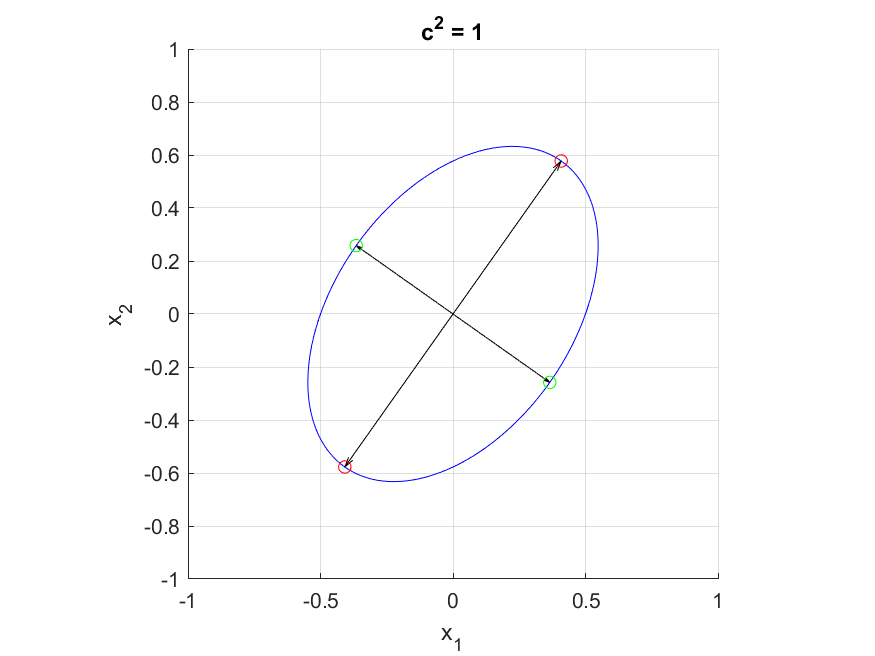
\includegraphics[scale=0.65]{./matlab/chapter-2/sol2.18.c1.png}
            \caption{When $c^2 = 1$}\label{fig:ellcis1}
        \end{figure}

        \begin{figure}[H]
            \centering
            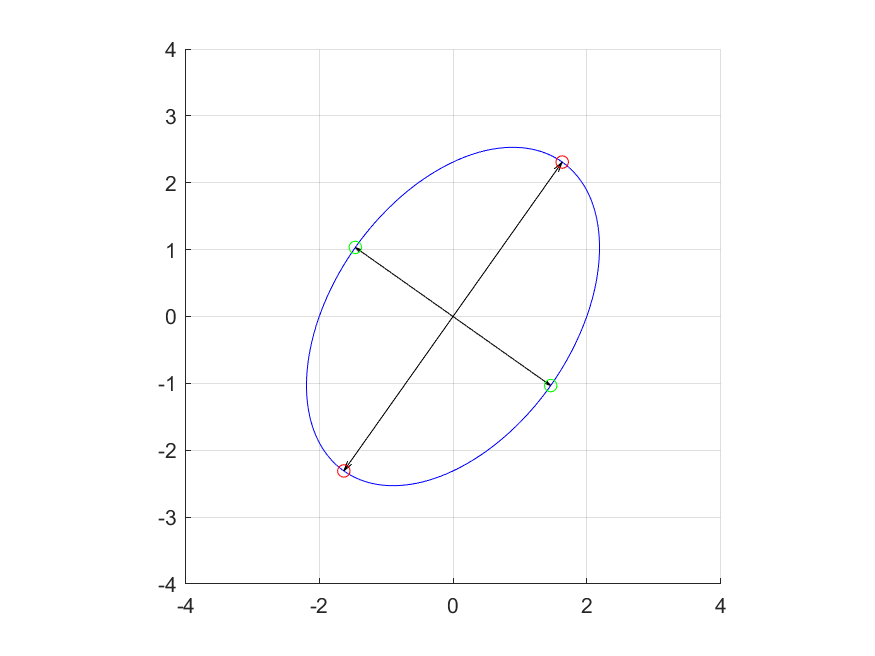
\includegraphics[scale=0.65]{./matlab/chapter-2/sol2.18.c4.png}
            \caption{When $c^2 = 4$}\label{fig:ellcis4}
        \end{figure}

        MATLAB code:
        \begin{lstlisting}
            A = [4 -sqrt(2); -sqrt(2) 3];
            [V,D] = eig(A);
            rref(A - D(1,1)*eye(width(A)))
            rref(A - D(2,2)*eye(width(A)))
            MyPlotEllipse(V,D,1,'sol2.18.c1')
            MyPlotEllipse(V,D,4,'sol2.18.c4')
        \end{lstlisting}

        \begin{lstlisting}
            function [] = MyPlotEllipse(V, D, c, fName)
    % Compute points corresponding to axis-oriented ellipse.
    % Where to center the ellipse.
    xc = 0;
    yc = 0;
    % The length in the major and minor axis.
    b = c/sqrt(D(1,1));
    a = c/sqrt(D(2,2));
    theta = acos(-V(:,1)'*[1 ; 0]); % acos(1/sqrt(3));
    
    t = linspace(0, 2*pi, 200);
    xt = b * cos(t) + xc;
    yt = a * sin(t) + yc;
    
    % Apply rotation by angle theta (in radians).
    cot = cos(theta); sit = sin(theta);
    x = xt * cot - yt * sit;
    y = xt * sit + yt * cot;

    hold on
        % Plot the ellipse.
        p=plot(x, y, '-', 'Color', 'blue');
        
        % Plot the vector for the major axis.
        quiver(0, 0, V(1,1), V(2,1), c, 'color', 'k');
        quiver(0, 0, -V(1,1), -V(2,1), c, 'color', 'k');
        
        % Plot the vector for the minor axis.
        quiver(0, 0, V(1,2), V(2,2), c, 'color', 'k');
        quiver(0, 0, -V(1,2), -V(2,2), c, 'color', 'k');
        
        % Plot red point for major axis.
        plot((c/sqrt(D(1,1)))*V(1,1), (c/sqrt(D(1,1)))*V(2,1), 'o', 'Color', 'red');
        plot(-(c/sqrt(D(1,1)))*V(1,1), -(c/sqrt(D(1,1)))*V(2,1), 'o', 'Color', 'red');
        
        % Plot green point for minor axis.
        plot((c/sqrt(D(2,2)))*V(1,2), (c/sqrt(D(2,2)))*V(2,2), 'o', 'Color', 'green');
        plot(-(c/sqrt(D(2,2)))*V(1,2), -(c/sqrt(D(2,2)))*V(2,2), 'o', 'Color', 'green');
        title(append('c^2 = ', num2str(c)))
        grid on
        pbaspect([1 1 1])
    hold off
    saved_file = append('.\applied-multivariate-statistics\solutions\chapter-2\', fName, '.png');
    saveas(p, saved_file, 'png')
end
        \end{lstlisting}
        % ------------------------------------------ %
        %                      (2.19)                %
        % ------------------------------------------ %
        \item[2.19] Let $\underset{\left(m \times m\right)}{\bold{A}^{1/2}} = \sum_{i=1}^m{\sqrt{\lambda_i} \bold{e}_i \bold{e}_i^\prime} = \bold{P}\bold{\Lambda}^{1/2}\bold{P}^\prime$, where $\bold{P}\bold{P}^\prime = \bold{P}^\prime\bold{P} = \bold{I}$. (The $\lambda_i$'s and the $\bold{e}$'s are the eigenvalues and associated normalized eigenvectors of the matrix $\bold{A}$.) Show Properties \textbf{(1)-(4)} of the square-root matrix in \textbf{(2-22)}.
        \begin{enumerate}
            \item[\textbf{(1)}]{${\left(\bold{A}^{1/2}\right)}^\prime = \bold{A}^{1/2}$ (that is, $\bold{A}$ is symmetric).}
            
            \[
                {\left(\bold{A}^{1/2}\right)}^\prime
                =
                {\left(\bold{P}\bold{\Lambda}^{1/2}\bold{P}^\prime\right)}^\prime
                \overset{\text{Exercise 2.3(c)}}{=}
                {\left(\bold{P}^\prime\right)}^\prime {\left(\bold{\Lambda}^{1/2}\right)}^\prime {\left(\bold{P}\right)}^\prime
                =
            \]
            \[
                =
                \bold{P} \bold{\Lambda}^{1/2} \bold{P}^\prime
                =
                \bold{A}^{1/2}
            \]

            \item[\textbf{(2)}]{$\bold{A}^{1/2}\bold{A}^{1/2} = \bold{A}$.}
            
            \[
                \bold{A}^{1/2}\bold{A}^{1/2} = 
                \left(\bold{P}\bold{\Lambda}^{1/2}\bold{P}^\prime\right)\left(\bold{P}\bold{\Lambda}^{1/2}\bold{P}^\prime\right)
                =
                \bold{P}\bold{\Lambda}^{1/2}\left(\bold{P}^\prime\bold{P}\right)\bold{\Lambda}^{1/2}\bold{P}^\prime
                =
            \]
            \[
                =
                \bold{P}\bold{\Lambda}^{1/2}\bold{I}\bold{\Lambda}^{1/2}\bold{P}^\prime
                =
                \bold{P}\bold{\Lambda}^{1/2}\bold{\Lambda}^{1/2}\bold{P}^\prime
                =
            \]
            \[
                =
                \bold{P}
                \begin{bmatrix}
                    \sqrt{\lambda_1} & 0 & \cdots & 0 \\
                    0 & \sqrt{\lambda_2} & \cdots & 0 \\
                    \vdots & \vdots & \ddots & \vdots \\
                    0 & 0 & \cdots & \sqrt{\lambda_m}
                \end{bmatrix}
                \begin{bmatrix}
                    \sqrt{\lambda_1} & 0 & \cdots & 0 \\
                    0 & \sqrt{\lambda_2} & \cdots & 0 \\
                    \vdots & \vdots & \ddots & \vdots \\
                    0 & 0 & \cdots & \sqrt{\lambda_m}
                \end{bmatrix}
                \bold{P}^\prime
                =
            \]
            \[
                \bold{P}
                \begin{bmatrix}
                    \lambda_1 & 0 & \cdots & 0 \\
                    0 & \lambda_2 & \cdots & 0 \\
                    \vdots & \vdots & \ddots & \vdots \\
                    0 & 0 & \cdots & \lambda_m
                \end{bmatrix}
                \bold{P}^\prime
                =
                \bold{P}
                \bold{\Lambda}
                \bold{P}^\prime
                =
                \bold{A}
            \]

            \item[\textbf{(3)}]{${\left(\bold{A}^{1/2}\right)}^{-1} = \sum_{i=1}^k{\frac{1}{\sqrt{\lambda_i}}\bold{e}_i\bold{e}_i^\prime} = \bold{P}\bold{\Lambda}^{-1/2}\bold{P}^\prime$, where $\bold{\Lambda}^{-1/2}$ is a diagonal matrix with $1/\sqrt{\lambda_i}$ as the ith diagonal element.}
            \newline
            \par
            First off, something useful,            
            \[
                \bold{\Lambda}^{-1/2}\bold{\Lambda}^{1/2}
                =
                \begin{bmatrix}
                    1/\sqrt{\lambda_1} & 0 & \cdots & 0 \\
                    0 & 1/\sqrt{\lambda_2} & \cdots & 0 \\
                    \vdots & \vdots & \ddots & \vdots \\
                    0 & 0 & \cdots & 1/\sqrt{\lambda_m}
                \end{bmatrix}
                \begin{bmatrix}
                    \sqrt{\lambda_1} & 0 & \cdots & 0 \\
                    0 & \sqrt{\lambda_2} & \cdots & 0 \\
                    \vdots & \vdots & \ddots & \vdots \\
                    0 & 0 & \cdots & \sqrt{\lambda_m}
                \end{bmatrix}
                =
                \bold{I}
            \]

            \[
                \bold{\Lambda}^{1/2}\bold{\Lambda}^{-1/2}
                =
                \begin{bmatrix}
                    \sqrt{\lambda_1} & 0 & \cdots & 0 \\
                    0 & \sqrt{\lambda_2} & \cdots & 0 \\
                    \vdots & \vdots & \ddots & \vdots \\
                    0 & 0 & \cdots & \sqrt{\lambda_m}
                \end{bmatrix}
                \begin{bmatrix}
                    1/\sqrt{\lambda_1} & 0 & \cdots & 0 \\
                    0 & 1/\sqrt{\lambda_2} & \cdots & 0 \\
                    \vdots & \vdots & \ddots & \vdots \\
                    0 & 0 & \cdots & 1/\sqrt{\lambda_m}
                \end{bmatrix}
                =
                \bold{I}
            \]

            We have $\bold{\Lambda}^{-1/2}\bold{\Lambda}^{1/2} = \bold{\Lambda}^{1/2}\bold{\Lambda}^{-1/2} = \bold{I}$, so $\bold{\Lambda}^{-1/2} = {\left(\bold{\Lambda}^{1/2}\right)}^{-1}$ is the inverse of $\bold{\Lambda}^{1/2}$ by \textbf{Definition 2A.27}.

            \[
                {\left(\bold{A}^{1/2}\right)}^{-1}
                =
                {\left(\bold{P}\bold{\Lambda}^{1/2}\bold{P}^\prime\right)}^{-1}
                \overset{Exercise 2.4(b)}{=}
                {\left(\bold{P}^\prime\right)}^{-1}{\left(\bold{\Lambda}^{1/2}\right)}^{-1}\bold{P}^{-1} 
                =
            \]
            \[
                \overset{\bold{P}^\prime = \bold{P}^{-1}}{=}
                {\left(\bold{P}^\prime\right)}^\prime{\left(\bold{\Lambda}^{1/2}\right)}^{-1}\bold{P}^\prime
                =
                \bold{P}{\left(\bold{\Lambda}^{1/2}\right)}^{-1}\bold{P}^\prime
            \]

            \[
                =
                \bold{P}\bold{\Lambda}^{-1/2}\bold{P}^\prime
                =
                \sum_{i=1}^m{\frac{1}{\sqrt{\lambda_i}}\bold{e}_i\bold{e}_i^\prime}
            \]

            \item[\textbf{(4)}]{$\bold{A}^{1/2}\bold{A}^{-1/2} = \bold{A}^{-1/2}\bold{A}^{1/2} = \bold{I}$, and $\bold{A}^{-1/2}\bold{A}^{-1/2} = \bold{A}^{-1}$, where $\bold{A}^{-1/2} = {\left(\bold{A}^{1/2}\right)}^{-1}$.}
            \par
            Above in \textbf{(3)} it was shown that $\bold{A}^{1/2}\bold{A}^{-1/2} = \bold{A}^{-1/2}\bold{A}^{1/2} = \bold{I}$, so $\bold{A}^{-1/2} = {\left(\bold{A}^{1/2}\right)}^{-1}$.
            \[
                \bold{A}^{-1/2}\bold{A}^{-1/2} 
                = 
                \begin{bmatrix}
                    1/\sqrt{\lambda_1} & 0 & \cdots & 0 \\
                    0 & 1/\sqrt{\lambda_2} & \cdots & 0 \\
                    \vdots & \vdots & \ddots & \vdots \\
                    0 & 0 & \cdots & 1/\sqrt{\lambda_m}
                \end{bmatrix}
                \begin{bmatrix}
                    1/\sqrt{\lambda_1} & 0 & \cdots & 0 \\
                    0 & 1/\sqrt{\lambda_2} & \cdots & 0 \\
                    \vdots & \vdots & \ddots & \vdots \\
                    0 & 0 & \cdots & 1/\sqrt{\lambda_m}
                \end{bmatrix}
                =
            \]
            \[
                =
                \begin{bmatrix}
                    1/\lambda_1 & 0 & \cdots & 0 \\
                    0 & 1/\lambda_2 & \cdots & 0 \\
                    \vdots & \vdots & \ddots & \vdots \\
                    0 & 0 & \cdots & 1/\lambda_m
                \end{bmatrix}
                =
                \bold{A}^{-1}
            \]

        \end{enumerate}
        % ------------------------------------------ %
        %                      (2.20)                %
        % ------------------------------------------ %
        \item[2.20] Determine the square-root matrix $\bold{A}^{1/2}$, using the matrix $\bold{A}$ in \textbf{Exercise 2.3}. Also, determine
        $\bold{A}^{-1/2}$, and show that $\bold{A}^{1/2}\bold{A}^{-1/2} = \bold{A}^{-1/2}\bold{A}^{1/2} = \bold{I}$.
        \par
        \[
            \bold{A}
            =
            \begin{bmatrix}
                2 & 1 \\
                1 & 3
            \end{bmatrix}
        \]
        \[
            0 = \left|\bold{A} - \lambda\bold{I}\right|
            =
            \left|
            \begin{matrix}
                2 - \lambda & 1 \\
                1 & 3 - \lambda
            \end{matrix}
            \right|
            =
            \left(2 - \lambda\right)\left(3 - \lambda\right) - 1
            =
            \lambda^2 - 5\lambda + 6 - 1
            =
        \]
        \[
            =
            \left(\lambda - \frac{5 - \sqrt{5}}{2}\right)\left(\lambda - \frac{5 + \sqrt{5}}{2}\right)
        \]
        The eigenvalues are $\left\{\lambda_1, \lambda_2\right\} = \left\{\frac{5 - \sqrt{5}}{2}, \frac{5 + \sqrt{5}}{2}\right\}$.
        \newline
        To sumplify things, define variables $a$ and $b$,
        \[
            a = {(5-\sqrt(5))}^{1/2}
        \]
        \[
            b = {(5+\sqrt(5))}^{1/2}
        \]
        Using a few useful facts,
        \[
            a^{1/2}(1 + 5^{1/2}) = 2b^{1/2}
        \]
        and
        \[
            b^{1/2}(1 - 5^{1/2}) = -2a^{1/2}
        \]
        \underline{$\lambda_1 = \frac{5 - \sqrt{5}}{2}$:}
        \[
            \bold{A}\bold{x}_1 = \lambda_1 \bold{x}_1
            \Rightarrow
            \begin{bmatrix}
                2 & 1 \\
                1 & 3
            \end{bmatrix}
            \begin{bmatrix}
                x_1 \\
                x_2
            \end{bmatrix}
            =
            \begin{bmatrix}
                \left(\frac{5 - \sqrt{5}}{2}\right)x_1 \\
                \left(\frac{5 - \sqrt{5}}{2}\right)x_2
            \end{bmatrix}
        \]
        \[
            \Rightarrow
            \begin{bmatrix}
                \left(\frac{-1 + \sqrt{5}}{2}\right) & 1 \\
                1 & \left(\frac{1 + \sqrt{5}}{2}\right)
            \end{bmatrix}
            \begin{bmatrix}
                x_1 \\
                x_2
            \end{bmatrix}
            =
            \begin{bmatrix}
                0 \\
                0
            \end{bmatrix}
        \]
        \[
            \begin{bmatrix}
                \left(\frac{-1 + \sqrt{5}}{2}\right) & 1 \\
                1 & \left(\frac{1 + \sqrt{5}}{2}\right)
            \end{bmatrix}
            \overset{\text{Row 2} - \left(\frac{2}{\sqrt{5} - 1}\right)\text{Row 1}}{\longrightarrow}
            \begin{bmatrix}
                \left(\frac{-1 + \sqrt{5}}{2}\right) & 1 \\
                0 & 0
            \end{bmatrix}
        \]
        So $\left(\frac{-1 + 5^{1/2}}{2}\right)x_1 + x_2 = 0 \Rightarrow x_2 
        = -\left(\frac{-1 + 5^{1/2}}{2}\right)x_1 = \left(\frac{1 - 5^{1/2}}{2}\right)x_1$
        \newline
        We have $x_2 = \left(\frac{1 - 5^{1/2}}{2}\right)x_1$, so when $x = -1$, $x_2 = -\left(\frac{1 - 5^{1/2}}{2}\right) > 0$.
        \[
            {\left\|\bold{x}_1\right\|} = \frac{{\left(5 - 5^{1/2}\right)^{1/2}}}{2^{1/2}} = \frac{a^{1/2}}{2^{1/2}}
        \]
        \[
            \bold{x}_1
            =
            \begin{bmatrix}
                -1 \\
                -\left(\frac{1 - 5^{1/2}}{2}\right)
            \end{bmatrix}
            \Rightarrow
            \bold{e}_1
            =
            \frac{\bold{x}_1}{\left\|\bold{x}_1\right\|}
            =
            \frac{2^{1/2}}{a^{1/2}}
            \begin{bmatrix}
                -1 \\
                -\left(\frac{1 - 5^{1/2}}{2}\right)
            \end{bmatrix}
            =
            \begin{bmatrix}
                -\frac{2^{1/2}}{a^{1/2}} \\
                -\left(\frac{1 - 5^{1/2}}{2^{1/2}a^{1/2}}\right)\left(\frac{1 + 5^{1/2}}{1 + 5^{1/2}}\right)
            \end{bmatrix}
            =
            \begin{bmatrix}
                -{\left(2/a\right)}^{1/2} \\
                {\left(2/b\right)}^{1/2}
            \end{bmatrix}
        \]
        \newline
        \underline{$\lambda_2 = \frac{5 + \sqrt{5}}{2}$:}
        \[
            \bold{A}\bold{x}_2 = \lambda_2 \bold{x}_2
            \Rightarrow
            \begin{bmatrix}
                2 & 1 \\
                1 & 3
            \end{bmatrix}
            \begin{bmatrix}
                x_1 \\
                x_2
            \end{bmatrix}
            =
            \begin{bmatrix}
                \left(\frac{5 + \sqrt{5}}{2}\right)x_1 \\
                \left(\frac{5 + \sqrt{5}}{2}\right)x_2
            \end{bmatrix}
        \]
        \[
            =
            \begin{bmatrix}
                \left(\frac{-1 - \sqrt{5}}{2}\right) & 1 \\
                1 & \left(\frac{1 - \sqrt{5}}{2}\right)
            \end{bmatrix}
            \begin{bmatrix}
                x_1 \\
                x_2
            \end{bmatrix}
            =
            \begin{bmatrix}
                0 \\
                0
            \end{bmatrix}
        \]
        \[
            \begin{bmatrix}
                \left(\frac{-1 - \sqrt{5}}{2}\right) & 1 \\
                1 & \left(\frac{1 - \sqrt{5}}{2}\right)
            \end{bmatrix}
            \overset{\text{Row 2} + \left(\frac{2}{1 + \sqrt{5}}\right)\text{Row 1}}{\longrightarrow}
            \begin{bmatrix}
                \left(\frac{-1 - \sqrt{5}}{2}\right) & 1 \\
                0 & 0
            \end{bmatrix}
        \]
        So $\left(\frac{-1 - \sqrt{5}}{2}\right)x_1 + x_2 = 0 \Rightarrow x_2 = \left(\frac{1 + \sqrt{5}}{2}\right)x_1$
        \newline
        We have $x_2 = \left(\frac{1 + 5^{1/2}}{2}\right)x_1$, so when $x = 1$, $x_2 = \left(\frac{1 + 5^{1/2}}{2}\right) > 0$.
        \[
            {\left\|\bold{x}_2\right\|} = \frac{{\left(5 + 5^{1/2}\right)}^{1/2}}{2^{1/2}} = \frac{b^{1/2}}{2^{1/2}}
        \]
        \[
            \bold{x}_2
            =
            \begin{bmatrix}
                1 \\
                \left(\frac{1 + 5^{1/2}}{2}\right)
            \end{bmatrix}
            \Rightarrow
            \bold{e}_1
            =
            \frac{\bold{x}_2}{\left\|\bold{x}_2\right\|}
            =
            \frac{2^{1/2}}{b^{1/2}}
            \begin{bmatrix}
                1 \\
                \left(\frac{1 + 5^{1/2}}{2}\right)
            \end{bmatrix}
            =
            \begin{bmatrix}
                \frac{2^{1/2}}{b^{1/2}} \\
                \left(\frac{1 + 5^{1/2}}{2^{1/2}b^{1/2}}\right) \left(\frac{1 - 5^{1/2}}{1 - 5^{1/2}}\right)
            \end{bmatrix}
            =
            \begin{bmatrix}
                {\left(2/b\right)}^{1/2} \\
                {\left(2/a\right)}^{1/2}
            \end{bmatrix}
        \]
        We finally have all of the eigenvalues and eigenvectors,
        \[
            \bold{\Lambda} 
            =
            \begin{bmatrix}
                \lambda_1 & 0 \\
                0 & \lambda_2
            \end{bmatrix}
            =
            \begin{bmatrix}
                a/2 & 0 \\
                0 & b/2
            \end{bmatrix}
        \]
        \[
            \bold{P}
            =
            \begin{bmatrix}
                \bold{e}_1 & \bold{e}_2
            \end{bmatrix}
            =
            \begin{bmatrix}
                {\left(2/a\right)}^{1/2} & {\left(2/b\right)}^{1/2} \\
                -{\left(2/b\right)}^{1/2} & {\left(2/a\right)}^{1/2}
            \end{bmatrix}
        \]
        Now to find $\bold{A}^{1/2}$. Rewrite a few things,
        
        \[
            \bold{A}^{1/2}
            =
            2^{1/2}
            \begin{bmatrix}
                {\left(b/a^2\right)}^{1/2} & {\left(a/b^2\right)}^{1/2} \\
                {\left(a/b^2\right)}^{1/2} & {\left(2^2/a\right)}^{1/2}
            \end{bmatrix}
        \]
        % ------------------------------------------ %
        %                      (2.21)                %
        % ------------------------------------------ %
        \item[2.21] (See \textbf{Result 2A.15}) Using the matrix
        \[
            \bold{A} = 
            \begin{bmatrix}
                1 & 1 \\
                2 & -2 \\
                2 & 2
            \end{bmatrix}
        \]
        \begin{enumerate}
            \item Calculate $\bold{A}^\prime\bold{A}$ and obtain the eigenvalues and eigenvectors.
            \par
            \[
                \bold{A}^\prime\bold{A}
                =
                \begin{bmatrix}
                    1 & 2 & 2 \\
                    1 & -2 & 2
                \end{bmatrix}
                \begin{bmatrix}
                    1 & 1 \\
                    2 & -2 \\
                    2 & 2
                \end{bmatrix}
                =
                \begin{bmatrix}
                    9 & 1 \\
                    1 & 9
                \end{bmatrix}
            \]
            
            \[
                0 = \left|\bold{A}^\prime\bold{A} - \lambda\bold{I}\right|
                =
                \left|
                \begin{matrix}
                    9 - \lambda & 1 \\
                    1 & 9 - \lambda
                \end{matrix}
                \right|
                =
                {\left(9 - \lambda\right)}^2 - 1
                =
                \lambda^2 - 18\lambda + 81 - 1
                = \left(\lambda - 8\right)\left(\lambda - 10\right)
            \]
            \[
                \left(\lambda_1^2, \lambda_1^2\right)
                =
                \left(8, 10\right)
            \]
            \underline{$\lambda_1^2 = 8$:}
            \[
                \bold{A}^\prime\bold{A}\bold{x}_1=\lambda_1^2\bold{x}_1
                \Rightarrow
                \begin{bmatrix}
                    9 & 1 \\
                    1 & 9
                \end{bmatrix}
                \begin{bmatrix}
                    x_1 \\
                    x_2
                \end{bmatrix}
                =
                \begin{bmatrix}
                    8x_1 \\
                    8x_2
                \end{bmatrix}
            \]
            \[
                \Rightarrow
                \begin{bmatrix}
                    1 & 1 \\
                    1 & 1
                \end{bmatrix}
                \begin{bmatrix}
                    x_1 \\
                    x_2
                \end{bmatrix}
                =
                \begin{bmatrix}
                    0 \\
                    0
                \end{bmatrix}
                \overset{\text{Row 2 - Row 1}}{\longrightarrow}
                \begin{bmatrix}
                    1 & 1 \\
                    0 & 0
                \end{bmatrix}
                \begin{bmatrix}
                    x_1 \\
                    x_2
                \end{bmatrix}
                =
                \begin{bmatrix}
                    0 \\
                    0
                \end{bmatrix}
            \]
            So $x_1 + x_2 = 0 \Rightarrow x_1 = -x_2$. Pick,
            \[
                \bold{x}_1
                =
                \begin{bmatrix}
                    1 \\
                    -1
                \end{bmatrix}
                \Rightarrow
                \bold{e}_1
                =
                \frac{\bold{x}_1}{\left\|\bold{x}_1\right\|}
                =
                \begin{bmatrix}
                    1/\sqrt{2} \\
                    -1/\sqrt{2}
                \end{bmatrix}
            \]
            \underline{$\lambda_2^2 = 10$:}
            \[
                \bold{A}^\prime\bold{A}\bold{x}_1=\lambda_1^2\bold{x}_1
                \Rightarrow
                \begin{bmatrix}
                    9 & 1 \\
                    1 & 9
                \end{bmatrix}
                \begin{bmatrix}
                    x_1 \\
                    x_2
                \end{bmatrix}
                =
                \begin{bmatrix}
                    10x_1 \\
                    10x_2
                \end{bmatrix}
            \]
            \[
                \Rightarrow
                \begin{bmatrix}
                    -1 & 1 \\
                    1 & -1
                \end{bmatrix}
                \begin{bmatrix}
                    x_1 \\
                    x_2
                \end{bmatrix}
                =
                \begin{bmatrix}
                    0 \\
                    0
                \end{bmatrix}
                \overset{\text{Row 2 + Row 1}}{\longrightarrow}
                \begin{bmatrix}
                    -1 & 1 \\
                    0 & 0
                \end{bmatrix}
                \begin{bmatrix}
                    x_1 \\
                    x_2
                \end{bmatrix}
                =
                \begin{bmatrix}
                    0 \\
                    0
                \end{bmatrix}
            \]
            So $-x_1 + x_2 = 0 \Rightarrow x_1 = x_2$. Pick,
            \[
                \bold{x}_1
                =
                \begin{bmatrix}
                    1 \\
                    1
                \end{bmatrix}
                \Rightarrow
                \bold{e}_2
                =
                \frac{\bold{x}_1}{\left\|\bold{x}_1\right\|}
                =
                \begin{bmatrix}
                    1/\sqrt{2} \\
                    1/\sqrt{2}
                \end{bmatrix}
            \]
            The eigenvectors are,
            \[
                \bold{V}
                =
                \begin{bmatrix}
                    1/\sqrt{2} & 1/\sqrt{2} \\
                    -1/\sqrt{2} & 1/\sqrt{2}
                \end{bmatrix}
            \]
            \item Calculate $\bold{A}\bold{A}^\prime$ and obtain the eigenvalues and eigenvectors. Check that the nonzero eigenvalues are the same as those in part a.
            \par
            \[
                \bold{A}\bold{A}^\prime
                =
                \begin{bmatrix}
                    1 & 1 \\
                    2 & -2 \\
                    2 & 2
                \end{bmatrix}
                \begin{bmatrix}
                    1 & 2 & 2 \\
                    1 & -2 & 2
                \end{bmatrix}
                =
                \begin{bmatrix}
                    2 & 0 & 4 \\
                    0 & 8 & 0 \\
                    4 & 0 & 8
                \end{bmatrix}
            \]
            
            \[
                0 = \left|\bold{A}\bold{A}^\prime - \lambda\bold{I}\right|
                =
                \left|
                \begin{matrix}
                    2 - \lambda & 0 & 4 \\
                    0 & 8 - \lambda & 0 \\
                    4 & 0 & 8 - \lambda
                \end{matrix}
                \right|
                =
                \left(2 - \lambda\right){\left(8 - \lambda\right)}^2 - 4\left(4\left(8 - \lambda\right)\right)
                =
            \]
            \[
                =
                \left(8 - \lambda\right)
                \left[\left(2 - \lambda\right){\left(8 - \lambda\right)} - 16\right]
                =
                \left(8 - \lambda\right)
                \left(\lambda^2 - 10\lambda\right)
                =
                \lambda\left(8 - \lambda\right)\left(\lambda - 10\right)
            \]
            \[
                \left(\lambda_1^2, \lambda_2^2, \lambda_2^2\right)
                =
                \left(0, 8, 10\right)
            \]
            Yes, these nonzero eigenvales are the same as those in part a.
            \newline
            \underline{$\lambda_1^2 = 0$:}
            \[
                \bold{A}\bold{A}^\prime\bold{x}_1=\lambda_1^2\bold{x}_1
                \Rightarrow
            \]
            \[
                \begin{bmatrix}
                    2 & 0 & 4 \\
                    0 & 8 & 0 \\
                    4 & 0 & 8
                \end{bmatrix}
                \begin{bmatrix}
                    x_1 \\
                    x_2 \\
                    x_3
                \end{bmatrix}
                =
                \begin{bmatrix}
                    0 \\
                    0 \\
                    0
                \end{bmatrix}
                \overset{\text{Row 3 - 2Row 1}}{\longrightarrow}
                \begin{bmatrix}
                    2 & 0 & 4 \\
                    0 & 8 & 0 \\
                    0 & 0 & 0
                \end{bmatrix}
                \begin{bmatrix}
                    x_1 \\
                    x_2 \\
                    x_3
                \end{bmatrix}
                =
                \begin{bmatrix}
                    0 \\
                    0 \\
                    0
                \end{bmatrix}
            \]
            So $2x_1 + 4x_3 = 0 \Rightarrow x_1 = -2x_3$ and $8x_2 = 0 \Rightarrow x_2 = 0$. Pick,
            \[
                \bold{x}_1
                =
                \begin{bmatrix}
                    -2 \\
                    0 \\
                    1
                \end{bmatrix}
                \Rightarrow
                \bold{e}_1
                =
                \frac{\bold{x}_1}{\left\|\bold{x}_1\right\|}
                =
                \begin{bmatrix}
                    -2/\sqrt{5} \\
                    0 \\
                    1/\sqrt{5}
                \end{bmatrix}
            \]
            \underline{$\lambda_2^2 = 8$:}
            \[
                \bold{A}\bold{A}^\prime\bold{x}_2=\lambda_2^2\bold{x}_2
                \Rightarrow
            \]
            \[
                \begin{bmatrix}
                    2 & 0 & 4 \\
                    0 & 8 & 0 \\
                    4 & 0 & 8
                \end{bmatrix}
                \begin{bmatrix}
                    x_1 \\
                    x_2 \\
                    x_3
                \end{bmatrix}
                =
                \begin{bmatrix}
                    8x_1 \\
                    8x_2 \\
                    8x_3
                \end{bmatrix}
            \]
            \[
                \Rightarrow
                \begin{bmatrix}
                    -6 & 0 & 4 \\
                    0 & 0 & 0 \\
                    4 & 0 & 0
                \end{bmatrix}
                \begin{bmatrix}
                    x_1 \\
                    x_2 \\
                    x_3
                \end{bmatrix}
                =
                \begin{bmatrix}
                    0 \\
                    0 \\
                    0
                \end{bmatrix}
            \]
            So $-6x_1 + 4x_3 = 0 \Rightarrow x_1 = 2/3x_3$ and $4x_1 = 0 \Rightarrow x_1 = 0$. Pick,
            \[
                \bold{x}_2
                =
                \begin{bmatrix}
                    0 \\
                    1 \\
                    0
                \end{bmatrix}
                \Rightarrow
                \bold{e}_1
                =
                \frac{\bold{x}_2}{\left\|\bold{x}_2\right\|}
                =
                \begin{bmatrix}
                    0 \\
                    1 \\
                    0
                \end{bmatrix}
            \]
            \underline{$\lambda_3^2 = 10$:}
            \[
                \bold{A}\bold{A}^\prime\bold{x}_2=\lambda_2^2\bold{x}_2
                \Rightarrow
            \]
            \[
                \begin{bmatrix}
                    2 & 0 & 4 \\
                    0 & 8 & 0 \\
                    4 & 0 & 8
                \end{bmatrix}
                \begin{bmatrix}
                    x_1 \\
                    x_2 \\
                    x_3
                \end{bmatrix}
                =
                \begin{bmatrix}
                    10x_1 \\
                    10x_2 \\
                    10x_3
                \end{bmatrix}
            \]
            \[
                \Rightarrow
                \begin{bmatrix}
                    -8 & 0 & 4 \\
                    0 & -2 & 0 \\
                    4 & 0 & -2
                \end{bmatrix}
                \begin{bmatrix}
                    x_1 \\
                    x_2 \\
                    x_3
                \end{bmatrix}
                =
                \begin{bmatrix}
                    0 \\
                    0 \\
                    0
                \end{bmatrix}
                \overset{\text{Row 3 + 1/2 Row 1}}{\longrightarrow}
                \begin{bmatrix}
                    -8 & 0 & 4 \\
                    0 & -2 & 0 \\
                    0 & 0 & 0
                \end{bmatrix}
                \begin{bmatrix}
                    x_1 \\
                    x_2 \\
                    x_3
                \end{bmatrix}
                =
                \begin{bmatrix}
                    0 \\
                    0 \\
                    0
                \end{bmatrix}
            \]
            So $-8x_1 + 4x_3 = 0 \Rightarrow x_3 = 2x_1$ and $-2x_2 = 0 \Rightarrow x_3 = 0$. Pick,
            \[
                \bold{x}_3
                =
                \begin{bmatrix}
                    1 \\
                    0 \\
                    2
                \end{bmatrix}
                \Rightarrow
                \bold{e}_1
                =
                \frac{\bold{x}_3}{\left\|\bold{x}_3\right\|}
                =
                \begin{bmatrix}
                    1/\sqrt{5} \\
                    0 \\
                    2/\sqrt{5}
                \end{bmatrix}
            \]
            The eigenvectors are,
            \[
                \bold{U}
                =
                \begin{bmatrix}
                    0 & 1/\sqrt{5} \\
                    1 & 0 \\
                    0 & 2/\sqrt{5}
                \end{bmatrix}
            \]
            \item Obtain the sigular-value decomposition of $\bold{A}$.
            \par
            \[
                \bold{A} = \bold{U}\bold{\Lambda}\bold{V}^\prime
                =
                \begin{bmatrix}
                    0 & 1/\sqrt{5} \\
                    1 & 0 \\
                    0 & 2/\sqrt{5}
                \end{bmatrix}
                \begin{bmatrix}
                    \sqrt{8} & 0 \\
                    0 & \sqrt{10}
                \end{bmatrix}
                \begin{bmatrix}
                    1/\sqrt{2} & -1/\sqrt{2} \\
                    1/\sqrt{2} & 1/\sqrt{2}
                \end{bmatrix}
                =
                \begin{bmatrix}
                    1 & 1 \\
                    2 & -2 \\
                    2 & 2
                \end{bmatrix}
                =
                \bold{A}
            \]
            \[
                \bold{A}
                =
                \sum_{k=1}^2{\lambda_k\bold{e}_k\bold{e}_k^\prime}
                =
                \sqrt{8}
                \begin{bmatrix}
                    0 \\
                    1 \\
                    0
                \end{bmatrix}
                \begin{bmatrix}
                    1/\sqrt{2} & -1/\sqrt{2}
                \end{bmatrix}
                +
                \sqrt{10}
                \begin{bmatrix}
                    1/\sqrt{5} \\
                    0 \\
                    2/\sqrt{5}
                \end{bmatrix}
                \begin{bmatrix}
                    1/\sqrt{2} & 1/\sqrt{2}
                \end{bmatrix}
                =
            \]
            \[
                =
                \sqrt{8}
                \begin{bmatrix}
                    0 & 0 \\
                    1/\sqrt{2} & -1/\sqrt{2} \\
                    0 & 0
                \end{bmatrix}
                +
                \sqrt{10}
                \begin{bmatrix}
                    1/\sqrt{10} & 1/\sqrt{10} \\
                    0 & 0 \\
                    2/\sqrt{10} & 2/\sqrt{10}
                \end{bmatrix}
                =
                \begin{bmatrix}
                    0 & 0 \\
                    2 & -2 \\
                    0 & 0
                \end{bmatrix}
                +
                \begin{bmatrix}
                    1 & 1 \\
                    0 & 0 \\
                    2 & 2
                \end{bmatrix}
                =
            \]
            \[
                =
                \begin{bmatrix}
                    1 & 1 \\
                    2 & -2 \\
                    2 & 2
                \end{bmatrix}
                =
                \bold{A}
            \]
        \end{enumerate}
        % ------------------------------------------ %
        %                      (2.22)                %
        % ------------------------------------------ %
        \item[2.22] (See \textbf{Result 2A.15}) Using the matrix
        \[
            \bold{A}
            =
            \begin{bmatrix}
                4 & 8 & 8 \\
                3 & 6 & -9
            \end{bmatrix}
        \]
        \begin{enumerate}
            \item Calculate $\bold{A}\bold{A}^\prime$ and obtain its eigenvalues and eigenvectors.
            \[
                \mathbf{A}\mathbf{A}^\prime
                =
                \begin{bmatrix}
                    4 & 8 & 8\\
                    3 & 6 & -9
                \end{bmatrix}
                \begin{bmatrix}
                    4 & 3 \\
                    8 & 6 \\
                    8 & -9
                \end{bmatrix}
                =
                \begin{bmatrix}
                    144 & -12 \\
                    -12 & 126
                \end{bmatrix}
                =
                6 \times
                \begin{bmatrix}
                    24 & -2 \\
                    -2 & 21
                \end{bmatrix}
            \]
            \[
                0 = \left|\mathbf{A}\mathbf{A}^\prime - \lambda^2\mathbf{I}\right| = \left|\mathbf{A}\mathbf{A}^\prime - \gamma\mathbf{I}\right|
                =
                \left|
                \begin{matrix}
                    24 - \gamma & -2 \\
                    -2 & 21 - \gamma
                \end{matrix}
                \right|
                =
            \]
            \[
                =
                (24-\gamma)(21-\gamma) - 4
                =
                504-45\gamma+\gamma^2-4
                =
                \gamma^2 - 45\gamma +500
                =
                (\gamma - 25)(\gamma - 20)
            \]
            The two eigenvalues are:
            \newline
            $\gamma_1=(1/6)\lambda_1^2= 20 \Rightarrow \lambda_1 = \sqrt{6 \times 20} = \sqrt{120}$
            \newline
            $\gamma_2=(1/6)\lambda_2^2= 25 \Rightarrow \lambda_2 = \sqrt{6 \times 25} = \sqrt{150}$
            \newline
            \newline
            \underline{For $\gamma_1 = 20$:}
            \[
                \mathbf{A}\mathbf{A}^\prime\mathbf{x}_1 = \gamma_1\mathbf{x}
                \Rightarrow
                \begin{bmatrix}
                    24 & -2 \\
                    -2 & 21
                \end{bmatrix}
                \begin{bmatrix}
                    x_1 \\
                    x_2
                \end{bmatrix}
                =
                \begin{bmatrix}
                    20 x_1\\
                    20 x_2
                \end{bmatrix}
                \Rightarrow
                \begin{bmatrix}
                    4 & -2 \\
                    -2 & 1
                \end{bmatrix}
                \begin{bmatrix}
                    x_1 \\
                    x_2
                \end{bmatrix}
                =
                \begin{bmatrix}
                    0 \\
                    0
                \end{bmatrix}
            \]
            \[
                \begin{bmatrix}
                    4 & -2 \\
                    -2 & 1
                \end{bmatrix}
                \begin{bmatrix}
                    x_1 \\
                    x_2
                \end{bmatrix}
                =
                \begin{bmatrix}
                    0 \\
                    0
                \end{bmatrix}
                \overset{\text{Row 2 + (1/2) Row 1}}{\longrightarrow}
                \begin{bmatrix}
                    4 & -2 \\
                    0 & 0
                \end{bmatrix}
                \begin{bmatrix}
                    x_1 \\
                    x_2
                \end{bmatrix}
                =
                \begin{bmatrix}
                    0 \\
                    0
                \end{bmatrix}
            \]
            So $4x_1 - 2x_2 = 0 \Rightarrow x_2 = 2x_1$
            \[
                \mathbf{x}_1
                =
                \begin{bmatrix}
                    1 \\
                    2
                \end{bmatrix}
                \Rightarrow
                \mathbf{u}_1
                =
                \frac{\mathbf{x}_1}{\left\|\mathbf{x}_1\right\|}
                =
                \begin{bmatrix}
                    1/\sqrt{5} \\
                    2/\sqrt{5}
                \end{bmatrix}
            \]
            \underline{For $\gamma_1 = 25$:}
            \[
                \mathbf{A}\mathbf{A}^\prime\mathbf{x}_2 = \gamma_2\mathbf{x}
                \Rightarrow
                \begin{bmatrix}
                    24 & -2 \\
                    -2 & 21
                \end{bmatrix}
                \begin{bmatrix}
                    x_1 \\
                    x_2
                \end{bmatrix}
                =
                \begin{bmatrix}
                    25 x_1\\
                    25 x_2
                \end{bmatrix}
                \Rightarrow
                \begin{bmatrix}
                    -1 & -2 \\
                    -2 & -4
                \end{bmatrix}
                \begin{bmatrix}
                    x_1 \\
                    x_2
                \end{bmatrix}
                =
                \begin{bmatrix}
                    0 \\
                    0
                \end{bmatrix}
            \]
            \[
                \begin{bmatrix}
                    -1 & -2 \\
                    -2 & -4
                \end{bmatrix}
                \begin{bmatrix}
                    x_1 \\
                    x_2
                \end{bmatrix}
                =
                \begin{bmatrix}
                    0 \\
                    0
                \end{bmatrix}
                \overset{\text{Row 2 - 2 Row 1}}{\longrightarrow}
                \begin{bmatrix}
                    -1 & -2 \\
                    0 & 0
                \end{bmatrix}
                \begin{bmatrix}
                    x_1 \\
                    x_2
                \end{bmatrix}
                =
                \begin{bmatrix}
                    0 \\
                    0
                \end{bmatrix}
            \]
            So $-x_1 - 2x_2 = 0 \Rightarrow x_1 = -2x_2$
            \[
                \mathbf{x}_1
                =
                \begin{bmatrix}
                    -2 \\
                    1
                \end{bmatrix}
                \Rightarrow
                \mathbf{u}_1
                =
                \frac{\mathbf{x}_1}{\left\|\mathbf{x}_1\right\|}
                =
                \begin{bmatrix}
                    -2/\sqrt{5} \\
                    1/\sqrt{5}
                \end{bmatrix}
            \]
            \[
                \Lambda
                =
                \begin{bmatrix}
                    \sqrt{120} & 0 \\
                    0 & \sqrt{150}
                \end{bmatrix}
                \hspace{0.2in}\text{and}\hspace{0.2in}
                \mathbf{U}
                =
                \begin{bmatrix}
                    \mathbf{u}_1 & \mathbf{u}_2
                \end{bmatrix}
                =
                \begin{bmatrix}
                    1/\sqrt{5} & -2/\sqrt{5} \\
                    2/\sqrt{5} & 1/\sqrt{5}
                \end{bmatrix}
            \]
            \item Calculate $\bold{A}^\prime\bold{A}$ and obtain its eigenvalues and eigenvectors. Check that the nonzero eigenvalues are the same as those in part a.
            \[
                \mathbf{A}^\prime\mathbf{A}
                =
                \begin{bmatrix}
                    4 & 3 \\
                    8 & 6 \\
                    8 & -9
                \end{bmatrix}
                \begin{bmatrix}
                    4 & 8 & 8\\
                    3 & 6 & -9
                \end{bmatrix}
                =
                \begin{bmatrix}
                    25 & 50 & 5 \\
                    50 & 100 & 10 \\
                    5 & 10 & 145
                \end{bmatrix}
                =
                5 \times
                \begin{bmatrix}
                    5 & 10 & 1 \\
                    10 & 20 & 2 \\
                    1 & 2 & 29
                \end{bmatrix}
            \]
            \[
                0 = \left|\mathbf{A}^\prime\mathbf{A} - \lambda^2\mathbf{I}\right| = \left|\mathbf{A}^\prime\mathbf{A} - \gamma\mathbf{I}\right|
                =
                \left|
                \begin{matrix}
                    5-\gamma & 10 & 1 \\
                    10 & 20-\gamma & 2 \\
                    1 & 2 & 29-\gamma
                \end{matrix}
                \right|
                =
            \]
            \[
                =
                (5-\gamma)[(20-\gamma)(29-\gamma) - 4] - 10[10(29-\gamma) - 2] + [20 - (20-\gamma)]
                =
            \]
            \[
                =
                (29\gamma^2 - 725\gamma + 2900)+(-\gamma^3 + 25\gamma^2 - 100\gamma) - 40 + 5\gamma - 2900 + 100\gamma + 40
                =
            \]
            \[
                =
                -\gamma(\gamma - 24)(\gamma - 30)
            \]
            The two nonzero eigenvalues are:
            \newline
            $\gamma_1=(1/5)\lambda_1^2= 24 \Rightarrow \lambda_1 = \sqrt{5 \times 24} = \sqrt{120}$
            \newline
            $\gamma_2=(1/5)\lambda_2^2= 30 \Rightarrow \lambda_2 = \sqrt{5 \times 30} = \sqrt{150}$
            \newline
            These are the same two eigenvalues as in part (a).
            \newline
            \newline
            \underline{For $\gamma_1 = 24$:}
            \[
                \mathbf{A}^\prime\mathbf{A}\mathbf{x}_1 = \gamma_1\mathbf{x}
                \Rightarrow
                \begin{bmatrix}
                    5 & 10 & 1 \\
                    10 & 20 & 2 \\
                    1 & 2 & 29
                \end{bmatrix}
                \begin{bmatrix}
                    x_1 \\
                    x_2 \\
                    x_3
                \end{bmatrix}
                =
                \begin{bmatrix}
                    24 x_1\\
                    24 x_2 \\
                    24 x_3
                \end{bmatrix}
                \Rightarrow
                \begin{bmatrix}
                    -19 & 10 & 1 \\
                    10 & -4 & 2 \\
                    1 & 2 & 5
                \end{bmatrix}
                \begin{bmatrix}
                    x_1 \\
                    x_2 \\
                    x_3
                \end{bmatrix}
                =
                \begin{bmatrix}
                    0 \\
                    0 \\
                    0
                \end{bmatrix}
            \]
            \[
                \begin{bmatrix}
                    -19 & 10 & 1 \\
                    10 & -4 & 2 \\
                    1 & 2 & 5
                \end{bmatrix}
                \overset{\text{Swap Row 1 with Row 3}}{\longrightarrow}
                \begin{bmatrix}
                    1 & 2 & 5 \\
                    10 & -4 & 2 \\
                    -19 & 10 & 1
                \end{bmatrix}
                \overset{\text{Row 3 + 19 Row 1}}{\longrightarrow}
                \begin{bmatrix}
                    1 & 2 & 5 \\
                    10 & -4 & 2 \\
                    0 & 48 & 96
                \end{bmatrix}
            \]
            \[
                \overset{\text{Row 2 - 10 Row 1}}{\longrightarrow}
                \begin{bmatrix}
                    1 & 2 & 5 \\
                    0 & -24 & -48 \\
                    0 & 48 & 96
                \end{bmatrix}
                \overset{\text{Simplify rows}}{\longrightarrow}
                \begin{bmatrix}
                    1 & 2 & 5 \\
                    0 & 1 & 2 \\
                    0 & 1 & 2
                \end{bmatrix}
                \overset{\text{Row 3 - Row 2}}{\longrightarrow}
            \]
            \[
                \begin{bmatrix}
                    1 & 2 & 5 \\
                    0 & 1 & 2 \\
                    0 & 0 & 0
                \end{bmatrix}
                \overset{\text{Row 1 - 2 Row 2}}{\longrightarrow}
                \begin{bmatrix}
                    1 & 0 & 1 \\
                    0 & 1 & 2 \\
                    0 & 0 & 0
                \end{bmatrix}
            \]
            So $x_1 + x_3 = 0 \Rightarrow x_1 = -x_3$
            and $x_2 + 2x_3 = 0 \Rightarrow x_2 = -2x_3$.

            \[
                \mathbf{x}_1
                =
                \begin{bmatrix}
                    -1 \\
                    -2 \\
                    1
                \end{bmatrix}
                \Rightarrow
                \mathbf{v}_1
                =
                \frac{\mathbf{x}_1}{\left\|\mathbf{x}_1\right\|}
                =
                \begin{bmatrix}
                    -1/\sqrt{6} \\
                    -2/\sqrt{6} \\
                    1/\sqrt{6}
                \end{bmatrix}
            \]
            \underline{For $\gamma_2 = 30$:}
            \[
                \mathbf{A}^\prime\mathbf{A}\mathbf{x}_1 = \gamma_1\mathbf{x}
                \Rightarrow
                \begin{bmatrix}
                    5 & 10 & 1 \\
                    10 & 20 & 2 \\
                    1 & 2 & 29
                \end{bmatrix}
                \begin{bmatrix}
                    x_1 \\
                    x_2 \\
                    x_3
                \end{bmatrix}
                =
                \begin{bmatrix}
                    30 x_1\\
                    30 x_2 \\
                    30 x_3
                \end{bmatrix}
                \Rightarrow
                \begin{bmatrix}
                    -25 & 10 & 1 \\
                    10 & -10 & 2 \\
                    1 & 2 & -1
                \end{bmatrix}
                \begin{bmatrix}
                    x_1 \\
                    x_2 \\
                    x_3
                \end{bmatrix}
                =
                \begin{bmatrix}
                    0 \\
                    0 \\
                    0
                \end{bmatrix}
            \]
            \[
                \begin{bmatrix}
                    -25 & 10 & 1 \\
                    10 & -10 & 2 \\
                    1 & 2 & -1
                \end{bmatrix}
                \overset{\text{Swap Row 1 with Row 3}}{\longrightarrow}
                \begin{bmatrix}
                    1 & 2 & -1 \\
                    10 & -10 & 2 \\
                    -25 & 10 & 1
                \end{bmatrix}
                \overset{\text{Row 3 + 25 Row 1}}{\longrightarrow}
                \begin{bmatrix}
                    1 & 2 & -1 \\
                    10 & -10 & 2 \\
                    0 & 60 & -24
                \end{bmatrix}
            \]
            \[
                \overset{\text{Row 2 - 10 Row 1}}{\longrightarrow}
                \begin{bmatrix}
                    1 & 2 & -1 \\
                    0 & -30 & 12 \\
                    0 & 48 & 96
                \end{bmatrix}
                \overset{\text{Simplify rows}}{\longrightarrow}
                \begin{bmatrix}
                    1 & 2 & -1 \\
                    0 & -5 & 2 \\
                    0 & 5 & -2
                \end{bmatrix}
                \overset{\text{Row 3 + Row 2}}{\longrightarrow}
            \]
            \[
                \begin{bmatrix}
                    1 & 2 & -1 \\
                    0 & -5 & 2 \\
                    0 & 0 & 0
                \end{bmatrix}
                \overset{\text{Row 1 - (2/5) Row 2}}{\longrightarrow}
                \begin{bmatrix}
                    1 & 0 & -1/5 \\
                    0 & -5 & 2 \\
                    0 & 0 & 0
                \end{bmatrix}
            \]
            So $x_1 - (1/5)x_3 = 0 \Rightarrow x_3 = 5x_1$
            and $-5x_2 + 2x_3 = 0 \Rightarrow x_2 = (2/5)x_3$.

            \[
                \mathbf{x}_2
                =
                \begin{bmatrix}
                    1 \\
                    2 \\
                    5
                \end{bmatrix}
                \Rightarrow
                \mathbf{v}_2
                =
                \frac{\mathbf{x}_2}{\left\|\mathbf{x}_2\right\|}
                =
                \begin{bmatrix}
                    1/\sqrt{30} \\
                    2/\sqrt{30} \\
                    5/\sqrt{30}
                \end{bmatrix}
            \]
            \[
                \Lambda
                =
                \begin{bmatrix}
                    \sqrt{120} & 0 \\
                    0 & \sqrt{150}
                \end{bmatrix}
                \hspace{0.2in}\text{and}\hspace{0.2in}
                \mathbf{V}
                =
                \begin{bmatrix}
                    \mathbf{v}_1 & \mathbf{v}_2
                \end{bmatrix}
                =
                \begin{bmatrix}
                    -1/\sqrt{6} & 1/\sqrt{30} \\
                    -2/\sqrt{6} & 2/\sqrt{30} \\
                    2/\sqrt{6} & 5/\sqrt{30}
                \end{bmatrix}
            \]
            \item Obtain the Singular value decomposition of $\bold{A}$.
            \newline
            \par
            Need to multiply SVD by -1, so we get the right result. Back when computing the eigenvalues notice the negative in front.
            \[
                \mathbf{A}
                =
                \mathbf{U}\mathbf{\Lambda}\mathbf{\mathbf{V}}^\prime
                =
                (-1)
                \begin{bmatrix}
                    1/\sqrt{5} & -2/\sqrt{5} \\
                    2/\sqrt{5} & 1/\sqrt{5}
                \end{bmatrix}
                \begin{bmatrix}
                    \sqrt{120} & 0 \\
                    0 & \sqrt{150}
                \end{bmatrix}
                \begin{bmatrix}
                    -1/\sqrt{6} & -2/\sqrt{6} & 2/\sqrt{6} \\
                    1/\sqrt{30} & 2/\sqrt{30} & 5/\sqrt{30}
                \end{bmatrix}
                =
            \]
            \[
                =
                \left(\frac{1}{\sqrt{5}}\right)
                \begin{bmatrix}
                    -1 & 2 \\
                    -2 & -1
                \end{bmatrix}
                \left(\sqrt{5}\sqrt{6}\right)
                \begin{bmatrix}
                    \sqrt{4} & 0 \\
                    0 & \sqrt{5}
                \end{bmatrix}
                \left(\frac{1}{\sqrt{6}}\right)
                \begin{bmatrix}
                    -1 & -2 & 1 \\
                    1/\sqrt{5} & 2/\sqrt{5} & 5/\sqrt{5}
                \end{bmatrix}
                =
            \]
            \[
                =
                \begin{bmatrix}
                    -1 & 2 \\
                    -2 & -1
                \end{bmatrix}
                \begin{bmatrix}
                    -2 & -4 & 2 \\
                    1 & 2 & 5
                \end{bmatrix}
                =
                \begin{bmatrix}
                    4 & 8 & 8 \\
                    3 & 6 & -9
                \end{bmatrix}
                =
                \mathbf{A}
            \]
        \end{enumerate}
        % ------------------------------------------ %
        %                      (2.23)                %
        % ------------------------------------------ %
        \item[2.23] Verify the relationships $\bold{V}^{1/2}\bm{\rho}\bold{V}^{1/2} = \bold{\Sigma}$ and $\bm{\rho} = {\left(\bold{V}^{1/2}\right)}^{-1}\bold{\Sigma}{\left(\bold{V}^{1/2}\right)}^{-1}$, where $\bold{\Sigma}$ is the
        $p \times p$ population covariance matrix [\textbf{Equation (2-32)}], $\bm{\rho}$ is the $p \times p$ population correlation
        matrix [\textbf{Equation (2-34)}], and $\bold{V}^{1/2}$ is the population standard deviation matrix
        [\textbf{Equation (2-35)}].
        \[
            \mathbf{V}^{1/2}\bm{\rho}\mathbf{V}^{1/2}
            =
            \begin{bmatrix}
                \sqrt{\sigma_{11}} & & 0 \\
                & \ddots & \\
                0 & & \sqrt{\sigma_{pp}}
            \end{bmatrix}
            \begin{bmatrix}
                \frac{\sigma_{11}}{\sqrt{\sigma_{11}}\sqrt{\sigma_{11}}} & \cdots & \frac{\sigma_{1p}}{\sqrt{\sigma_{11}}\sqrt{\sigma_{pp}}} \\
                \vdots & \ddots & \vdots \\
                \frac{\sigma_{p1}}{\sqrt{\sigma_{pp}}\sqrt{\sigma_{11}}} & \cdots & \frac{\sigma_{pp}}{\sqrt{\sigma_{pp}}\sqrt{\sigma_{pp}}}
            \end{bmatrix}
            \begin{bmatrix}
                \sqrt{\sigma_{11}} & & 0 \\
                & \ddots & \\
                0 & & \sqrt{\sigma_{pp}}
            \end{bmatrix}
            =
        \]
        \[
            =
            \begin{bmatrix}
                \frac{\sigma_{11}}{\sqrt{\sigma_{11}}} & \cdots & \frac{\sigma_{1p}}{\sqrt{\sigma_{pp}}} \\
                \vdots & \ddots & \vdots \\
                \frac{\sigma_{p1}}{\sqrt{\sigma_{11}}} & \cdots & \frac{\sigma_{pp}}{\sqrt{\sigma_{pp}}}
            \end{bmatrix}
            \begin{bmatrix}
                \sqrt{\sigma_{11}} & & 0 \\
                & \ddots & \\
                0 & & \sqrt{\sigma_{pp}}
            \end{bmatrix}
            =
            \begin{bmatrix}
                \sigma_{11} & \cdots & \sigma_{1p} \\
                \vdots & \ddots & \vdots \\
                \sigma_{p1} & \cdots & \sigma_{pp}
            \end{bmatrix}
            =
            \mathbf{\Sigma}
        \]
        \[
            {\left(\bold{V}^{1/2}\right)}^{-1}\bold{\Sigma}{\left(\bold{V}^{1/2}\right)}^{-1}
            =
        \]
        \[
            =
            {\left(
                \begin{bmatrix}
                    \sqrt{\sigma_{11}} & & 0 \\
                    & \ddots & \\
                    0 & & \sqrt{\sigma_{pp}}
                \end{bmatrix}
            \right)}^{-1}
            \begin{bmatrix}
                \sigma_{11} & \cdots & \sigma_{1p} \\
                \vdots & \ddots & \vdots \\
                \sigma_{p1} & \cdots & \sigma_{pp}
            \end{bmatrix}
            {\left(
                \begin{bmatrix}
                    \sqrt{\sigma_{11}} & & 0 \\
                    & \ddots & \\
                    0 & & \sqrt{\sigma_{pp}}
                \end{bmatrix}
            \right)}^{-1}
            =
        \]
        \[
            =
            \begin{bmatrix}
                1/\sqrt{\sigma_{11}} & & 0 \\
                & \ddots & \\
                0 & & 1/\sqrt{\sigma_{pp}}
            \end{bmatrix}
            \begin{bmatrix}
                \sigma_{11} & \cdots & \sigma_{1p} \\
                \vdots & \ddots & \vdots \\
                \sigma_{p1} & \cdots & \sigma_{pp}
            \end{bmatrix}
            \begin{bmatrix}
                1/\sqrt{\sigma_{11}} & & 0 \\
                & \ddots & \\
                0 & & 1/\sqrt{\sigma_{pp}}
            \end{bmatrix}
            =
        \]
        \[
            =
            \begin{bmatrix}
                1/\sqrt{\sigma_{11}} & & 0 \\
                & \ddots & \\
                0 & & 1/\sqrt{\sigma_{pp}}
            \end{bmatrix}
            \begin{bmatrix}
                \frac{\sigma_{11}}{\sqrt{\sigma_{11}}} & \cdots & \frac{\sigma_{1p}}{\sqrt{\sigma_{pp}}} \\
                \vdots & \ddots & \vdots \\
                \frac{\sigma_{p1}}{\sqrt{\sigma_{11}}} & \cdots & \frac{\sigma_{pp}}{\sqrt{\sigma_{pp}}}
            \end{bmatrix}
            =
        \]
        \[
            =
            \begin{bmatrix}
                \frac{\sigma_{11}}{\sqrt{\sigma_{11}}\sqrt{\sigma_{11}}} & \cdots & \frac{\sigma_{1p}}{\sqrt{\sigma_{11}}\sqrt{\sigma_{pp}}} \\
                \vdots & \ddots & \vdots \\
                \frac{\sigma_{p1}}{\sqrt{\sigma_{pp}}\sqrt{\sigma_{11}}} & \cdots & \frac{\sigma_{pp}}{\sqrt{\sigma_{pp}}\sqrt{\sigma_{pp}}}
            \end{bmatrix}
            = \bm{\rho}
        \]
        % ------------------------------------------ %
        %                      (2.24)                %
        % ------------------------------------------ %
        \item[2.24] Let $\bold{X}$ have covariance matrix
        \[
            \bold{\Sigma}
            =
            \begin{bmatrix}
                4 & 0 & 0\\
                0 & 9 & 0\\
                0 & 0 & 1
            \end{bmatrix}
        \]
        Find
        \begin{enumerate}
            \item $\bold{\Sigma}^{-1}$
            \par
            Using what's on page 59, the inverse of a diagonal matrix is the reciprocal of the elements.
            \[
                \mathbf{\Sigma}^{-1}
                =
                \begin{bmatrix}
                    1/4 & 0 & 0 \\
                    0 & 1/9 & 0 \\
                    0 & 0 & 1
                \end{bmatrix}
            \]
            \item The eigenvalues and eigenvectors of $\bold{\Sigma}$.
            \[
                 0 = \left|\mathbf{\Sigma} - \lambda\mathbf{I}\right|
                 =
                 \begin{bmatrix}
                    4-\lambda & 0 & 0 \\
                    0 & 9-\lambda & 0 \\
                    0 & 0 & 1-\lambda
                 \end{bmatrix}
                 =
                 \left(4-\lambda\right)\left(9-\lambda\right)\left(1-\lambda\right)
            \]
            The eigenvalues are simply the diagonal elements of $\mathbf{\Sigma}$, $\left(\lambda_1, \lambda_2, \lambda_3\right) = \left(1,4,9\right)$.
            \newline
            \underline{$\lambda_1 = 1$:}
            \[
                \mathbf{\Sigma}\mathbf{x}_1 = \lambda_1\mathbf{x}_1
                \Rightarrow
                \begin{bmatrix}
                    4 & 0 & 0\\
                    0 & 9 & 0\\
                    0 & 0 & 1
                \end{bmatrix}
                \begin{bmatrix}
                    x_1 \\
                    x_2 \\
                    x_3
                \end{bmatrix}
                =
                \begin{bmatrix}
                    x_1 \\
                    x_2 \\
                    x_3
                \end{bmatrix}
            \]
            \[
                \Rightarrow
                \begin{bmatrix}
                    3 & 0 & 0\\
                    0 & 8 & 0\\
                    0 & 0 & 0
                \end{bmatrix}
                \begin{bmatrix}
                    x_1 \\
                    x_2 \\
                    x_3
                \end{bmatrix}
                =
                \begin{bmatrix}
                    0 \\
                    0 \\
                    0
                \end{bmatrix}
            \]
            So $x_1 = x_2 = 0$ and $x_3$ is free.
            \[
                \mathbf{x}_1
                =
                \mathbf{e}_1
                =
                \begin{bmatrix}
                    0 \\
                    0 \\
                    1
                \end{bmatrix}
            \]
            \underline{$\lambda_2 = 4$:}
            \[
                \mathbf{\Sigma}\mathbf{x}_2 = \lambda_2\mathbf{x}_2
                \Rightarrow
                \begin{bmatrix}
                    4 & 0 & 0\\
                    0 & 9 & 0\\
                    0 & 0 & 1
                \end{bmatrix}
                \begin{bmatrix}
                    x_1 \\
                    x_2 \\
                    x_3
                \end{bmatrix}
                =
                \begin{bmatrix}
                    4x_1 \\
                    4x_2 \\
                    4x_3
                \end{bmatrix}
            \]
            \[
                \Rightarrow
                \begin{bmatrix}
                    0 & 0 & 0\\
                    0 & 5 & 0\\
                    0 & 0 & -3
                \end{bmatrix}
                \begin{bmatrix}
                    x_1 \\
                    x_2 \\
                    x_3
                \end{bmatrix}
                =
                \begin{bmatrix}
                    0 \\
                    0 \\
                    0
                \end{bmatrix}
            \]
            So $x_2 = x_3 = 0$ and $x_1$ is free.
            \[
                \mathbf{x}_2
                =
                \mathbf{e}_2
                =
                \begin{bmatrix}
                    1 \\
                    0 \\
                    0
                \end{bmatrix}
            \]
            \underline{$\lambda_3 = 9$:}
            \[
                \mathbf{\Sigma}\mathbf{x}_3 = \lambda_3\mathbf{x}_3
                \Rightarrow
                \begin{bmatrix}
                    4 & 0 & 0\\
                    0 & 9 & 0\\
                    0 & 0 & 1
                \end{bmatrix}
                \begin{bmatrix}
                    x_1 \\
                    x_2 \\
                    x_3
                \end{bmatrix}
                =
                \begin{bmatrix}
                    9x_1 \\
                    9x_2 \\
                    9x_3
                \end{bmatrix}
            \]
            \[
                \Rightarrow
                \begin{bmatrix}
                    -5 & 0 & 0\\
                    0 & 0 & 0\\
                    0 & 0 & -8
                \end{bmatrix}
                \begin{bmatrix}
                    x_1 \\
                    x_2 \\
                    x_3
                \end{bmatrix}
                =
                \begin{bmatrix}
                    0 \\
                    0 \\
                    0
                \end{bmatrix}
            \]
            So $x_1 = x_3 = 0$ and $x_2$ is free.
            \[
                \mathbf{x}_3
                =
                \mathbf{e}_3
                =
                \begin{bmatrix}
                    0 \\
                    1 \\
                    0
                \end{bmatrix}
            \]
            Putting it all together,
            \[
                \mathbf{\Lambda}
                =
                \begin{bmatrix}
                    1 & 0 & 0 \\
                    0 & 4 & 0 \\
                    0 & 0 & 9
                \end{bmatrix}
                \hspace{0.2in}\text{and}\hspace{0.2in}
                \mathbf{P}
                =
                \begin{bmatrix}
                    0 & 1 & 0 \\
                    0 & 0 & 1 \\
                    1 & 0 & 0
                \end{bmatrix}
            \]
            \par
            The eigenvalues are the elements in the diagonal matrix and the eigenvectors are the identity matrix.
            \item The eigenvalues and eigenvectors of $\bold{\Sigma}^{-1}$.
            \[
                 0 = \left|\mathbf{\Sigma} - \lambda\mathbf{I}\right|
                 =
                 \begin{bmatrix}
                    1/4-\lambda & 0 & 0 \\
                    0 & 1/9-\lambda & 0 \\
                    0 & 0 & 1-\lambda
                 \end{bmatrix}
                 =
                 \left(1/4-\lambda\right)\left(1/9-\lambda\right)\left(1/9-\lambda\right)
            \]
            The eigenvalues are simply the diagonal elements of $\mathbf{\Sigma}$, $\left(\lambda_1, \lambda_2, \lambda_3\right) = \left(1/9,1/4,1\right)$.
            \newline
            \newline
            \underline{$\lambda_1 = 1/9$:}
            \[
                \mathbf{\Sigma}\mathbf{x}_1 = \lambda_1\mathbf{x}_1
                \Rightarrow
                \begin{bmatrix}
                    1/4 & 0 & 0\\
                    0 & 1/9 & 0\\
                    0 & 0 & 1
                \end{bmatrix}
                \begin{bmatrix}
                    x_1 \\
                    x_2 \\
                    x_3
                \end{bmatrix}
                =
                \begin{bmatrix}
                    (1/9)x_1 \\
                    (1/9)x_2 \\
                    (1/9)x_3
                \end{bmatrix}
            \]
            \[
                \Rightarrow
                \begin{bmatrix}
                    5/36 & 0 & 0\\
                    0 & 0 & 0\\
                    0 & 0 & 8/9
                \end{bmatrix}
                \begin{bmatrix}
                    x_1 \\
                    x_2 \\
                    x_3
                \end{bmatrix}
                =
                \begin{bmatrix}
                    0 \\
                    0 \\
                    0
                \end{bmatrix}
            \]
            So $x_1 = x_3 = 0$ and $x_2$ is free.
            \[
                \mathbf{x}_1
                =
                \mathbf{e}_1
                =
                \begin{bmatrix}
                    0 \\
                    1 \\
                    0
                \end{bmatrix}
            \]
            \underline{$\lambda_2 = 1/4$:}
            \[
                \mathbf{\Sigma}\mathbf{x}_2 = \lambda_1\mathbf{x}_2
                \Rightarrow
                \begin{bmatrix}
                    1/4 & 0 & 0\\
                    0 & 1/9 & 0\\
                    0 & 0 & 1
                \end{bmatrix}
                \begin{bmatrix}
                    x_1 \\
                    x_2 \\
                    x_3
                \end{bmatrix}
                =
                \begin{bmatrix}
                    (1/4)x_1 \\
                    (1/4)x_2 \\
                    (1/4)x_3
                \end{bmatrix}
            \]
            \[
                \Rightarrow
                \begin{bmatrix}
                    0 & 0 & 0\\
                    0 & -5/36 & 0\\
                    0 & 0 & 3/4
                \end{bmatrix}
                \begin{bmatrix}
                    x_1 \\
                    x_2 \\
                    x_3
                \end{bmatrix}
                =
                \begin{bmatrix}
                    0 \\
                    0 \\
                    0
                \end{bmatrix}
            \]
            So $x_2 = x_3 = 0$ and $x_1$ is free.
            \[
                \mathbf{x}_2
                =
                \mathbf{e}_2
                =
                \begin{bmatrix}
                    1 \\
                    0 \\
                    0
                \end{bmatrix}
            \]
            \underline{$\lambda_3 = 1$:}
            \[
                \mathbf{\Sigma}\mathbf{x}_3 = \lambda_3\mathbf{x}_3
                \Rightarrow
                \begin{bmatrix}
                    1/4 & 0 & 0\\
                    0 & 1/9 & 0\\
                    0 & 0 & 1
                \end{bmatrix}
                \begin{bmatrix}
                    x_1 \\
                    x_2 \\
                    x_3
                \end{bmatrix}
                =
                \begin{bmatrix}
                    x_1 \\
                    x_2 \\
                    x_3
                \end{bmatrix}
            \]
            \[
                \Rightarrow
                \begin{bmatrix}
                    -3/4 & 0 & 0\\
                    0 & -8/9 & 0\\
                    0 & 0 & 0
                \end{bmatrix}
                \begin{bmatrix}
                    x_1 \\
                    x_2 \\
                    x_3
                \end{bmatrix}
                =
                \begin{bmatrix}
                    0 \\
                    0 \\
                    0
                \end{bmatrix}
            \]
            So $x_1 = x_2 = 0$ and $x_3$ is free.
            \[
                \mathbf{x}_3
                =
                \mathbf{e}_3
                =
                \begin{bmatrix}
                    0 \\
                    0 \\
                    1
                \end{bmatrix}
            \]
            Putting it all together,
            \[
                \mathbf{\Lambda}
                =
                \begin{bmatrix}
                    1/9 & 0 & 0 \\
                    0 & 1/4 & 0 \\
                    0 & 0 & 1
                \end{bmatrix}
                \hspace{0.2in}\text{and}\hspace{0.2in}
                \mathbf{P}
                =
                \begin{bmatrix}
                    0 & 1 & 0 \\
                    1 & 0 & 0 \\
                    0 & 0 & 1
                \end{bmatrix}
            \]
            \par
            The eigenvalues are the elements in the diagonal matrix and the eigenvectors are the identity matrix.
        \end{enumerate}
        % ------------------------------------------ %
        %                      (2.25)                %
        % ------------------------------------------ %
        \item[2.25] Let $\bold{X}$ have covariance matrix
        \[
            \bold{\Sigma}
            =
            \begin{bmatrix}
                25 & -2 & 4 \\
                -2 & 4 & 1 \\
                4 & 1 & 9
            \end{bmatrix}
        \]
        \begin{enumerate}
            \item Determine $\bm{\rho}$ and $\bold{V}^{1/2}$.
            \[
                \bm{\rho}
                =
                \begin{bmatrix}
                    \frac{\sigma_{11}}{\sqrt{\sigma_{11}}\sqrt{\sigma_{11}}} & \frac{\sigma_{12}}{\sqrt{\sigma_{11}}\sqrt{\sigma_{22}}} & \frac{\sigma_{13}}{\sqrt{\sigma_{11}}\sqrt{\sigma_{33}}} \\
                    \frac{\sigma_{21}}{\sqrt{\sigma_{22}}\sqrt{\sigma_{11}}} & \frac{\sigma_{22}}{\sqrt{\sigma_{22}}\sqrt{\sigma_{22}}} & \frac{\sigma_{23}}{\sqrt{\sigma_{22}}\sqrt{\sigma_{33}}} \\
                    \frac{\sigma_{31}}{\sqrt{\sigma_{33}}\sqrt{\sigma_{11}}} & \frac{\sigma_{32}}{\sqrt{\sigma_{33}}\sqrt{\sigma_{22}}} & \frac{\sigma_{33}}{\sqrt{\sigma_{33}}\sqrt{\sigma_{33}}}
                \end{bmatrix}
                =
            \]
            \[
                =
                \begin{bmatrix}
                    \frac{25}{\sqrt{25}\sqrt{25}} & \frac{-2}{\sqrt{25}\sqrt{4}} & \frac{4}{\sqrt{25}\sqrt{9}} \\
                    \frac{-2}{\sqrt{4}\sqrt{25}} & \frac{4}{\sqrt{4}\sqrt{4}} & \frac{1}{\sqrt{4}\sqrt{9}} \\
                    \frac{4}{\sqrt{9}\sqrt{25}} & \frac{1}{\sqrt{9}\sqrt{4}} & \frac{9}{\sqrt{9}\sqrt{9}}
                \end{bmatrix}
                =
                \begin{bmatrix}
                    1 & -1/5 & 4/15 \\
                    -1/5 & 1 & 1/6 \\
                    4/15 & 1/6 & 1
                \end{bmatrix}
            \]
            \item Multiply your matrices to check the relation $\bold{V}^{1/2}\bm{\rho}\bold{V}^{1/2} = \bold{\Sigma}$.
            \[
                \bold{V}^{1/2}\bm{\rho}\bold{V}^{1/2} 
                = 
                \begin{bmatrix}
                5 & 0 & 0 \\
                0 & 2 & 0 \\
                0 & 0 & 3   
                \end{bmatrix}
                \begin{bmatrix}
                    1 & -1/5 & 4/15 \\
                    -1/5 & 1 & 1/6 \\
                    4/15 & 1/6 & 1
                \end{bmatrix}
                \begin{bmatrix}
                    5 & 0 & 0 \\
                    0 & 2 & 0 \\
                    0 & 0 & 3   
                \end{bmatrix}
                =
            \]
            \[
                =
                \begin{bmatrix}
                    5 & -1 & 4/3 \\
                    -2/5 & 2 & 1/3 \\
                    4/5 & 1/2 & 3
                \end{bmatrix}
                \begin{bmatrix}
                    5 & 0 & 0 \\
                    0 & 2 & 0 \\
                    0 & 0 & 3   
                \end{bmatrix}
                =
                \begin{bmatrix}
                    25 & -2 & 4 \\
                    -2 & 4 & 1 \\
                    4 & 1 & 9
                \end{bmatrix}
            \]
        \end{enumerate}
        % ------------------------------------------ %
        %                      (2.26)                %
        % ------------------------------------------ %
        \item[2.26] Use $\bold{\Sigma}$ as given in Exercise 2.25.
        \begin{enumerate}
            \item Find $\rho_{13}$.
            \par
            We can pick $\rho_{13}$ off the result from Exercise 2.25 (a),
            \[
                \rho_{13} = 4/15
            \]
            \item Find the correlation between $X_1$ and $\frac{1}{2}X_2 + \frac{1}{2}X_3$.
            \par
            \[
                \mathbf{X}
                =
                \begin{bNiceMatrix}[margin]
                    \mathbf{X}^{(1)} \\
                    \mathbf{X}^{(2)}
                    \CodeAfter \tikz \draw[dotted] (2-|1) -- (2-|last);
                \end{bNiceMatrix}
            \]
            \[
                \mathbf{X}^{(1)}
                =
                \begin{bmatrix}
                    X_1
                \end{bmatrix}
                \hspace{0.2in}\text{and}\hspace{0.2in}
                \mathbf{X}^{(2)}
                =
                \begin{bmatrix}
                    X_2 \\
                    X_3
                \end{bmatrix}
            \]
            \[
                Y 
                = 
                \frac{1}{2}X_1 + \frac{1}{2}X_2
                =
                \begin{bmatrix}
                    1/2 & 1/2
                \end{bmatrix}
                \begin{bmatrix}
                    X_1 \\
                    X_2
                \end{bmatrix}
                =
                \mathbf{c}^\prime
                \mathbf{X}^{(2)}
            \]
            So $\mathbf{c} = \begin{bmatrix}
                1/2 \\
                1/2
            \end{bmatrix}$.
            \[
                \bold{\Sigma}
                =
                \begin{bNiceMatrix}[margin]
                    25 & -2 & 4 \\
                    -2 & 4 & 1 \\
                    4 & 1 & 9
                    \CodeAfter \tikz \draw[dotted] (2-|1) -- (2-|last) \and (1-|2) -- (last-|2) ;
                \end{bNiceMatrix}
                        =
                \begin{bNiceMatrix}[margin]
                    \bm{\Sigma}_{11} & \bm{\Sigma}_{12} \\
                    \bm{\Sigma}_{21} & \bm{\Sigma}_{22}
                    \CodeAfter \tikz \draw[dotted] (2-|1) -- (2-|last) \and (1-|2) -- (last-|2);
                \end{bNiceMatrix}
                =
            \]
            % \[
            %     \bold{\Sigma}
            %     =
            %     \left[
            %     \begin{array}{c;{2pt/2pt}cc}
            %         25 & -2 & 4 \\
            %         \hdashline[3pt/3pt]
            %         -2 & 4 & 1 \\
            %         4 & 1 & 9
            %     \end{array}
            %     \right]
            %     =
            %     \left[
            %     \begin{array}{c;{2pt/2pt}c}
            %         \bm{\Sigma}_{11} & \bm{\Sigma}_{12} \\
            %         \hdashline[3pt/3pt]
            %         \bm{\Sigma}_{21} & \bm{\Sigma}_{22} \\
            %     \end{array}
            %     \right]
            %     =
            % \]
            % \[
            %     \left[
            %     \begin{array}{c;{2pt/2pt}c}
            %         \text{Cov}\left(\textbf{X}^{(1)}, \textbf{X}^{(1)}\right) & \text{Cov}\left(\textbf{X}^{(1)}, \textbf{X}^{(2)}\right) \\
            %         \hdashline[3pt/3pt] \\
            %         \text{Cov}\left(\textbf{X}^{(2)}, \textbf{X}^{(1)}\right) & \text{Cov}\left(\textbf{X}^{(2)}, \textbf{X}^{(2)}\right)
            %     \end{array}
            %     \right]
            % \]
            \[
                \text{Cov}\left(\mathbf{X}^{(1)}, Y\right)
                =
                \text{Cov}\left(\mathbf{X}^{(1)}, \mathbf{c}^\prime
                \mathbf{X}^{(2)}\right)
                =
            \]
            \[
                =
                E\left[\left(\mathbf{X}^{(1)} - E\left[\mathbf{X}^{(1)}\right]\right){\left(\mathbf{c}^\prime\mathbf{X}^{(2)} - E\left[\mathbf{c}^\prime\mathbf{X}^{(2)}\right]\right)}^\prime\right]
                =
            \]
            \[
                =
                E\left[\left(\mathbf{X}^{(1)} - E\left[\mathbf{X}^{(1)}\right]\right){\left(\mathbf{c}^\prime\mathbf{X}^{(2)} - \mathbf{c}^\prime E\left[\mathbf{X}^{(2)}\right]\right)}^\prime\right]
                =
            \]
            \[
                =
                E\left[\left(\mathbf{X}^{(1)} - E\left[\mathbf{X}^{(1)}\right]\right)\left\{\mathbf{c}^\prime\left(\mathbf{X}^{(2)} - E\left[\mathbf{X}^{(2)}\right]\right)\right\}^\prime\right]
                =
            \]
            \[
                =
                E\left[\left(\mathbf{X}^{(1)} - E\left[\mathbf{X}^{(1)}\right]\right)\left\{\left(\mathbf{X}^{(2)} - E\left[\mathbf{X}^{(2)}\right]\right)\right\}^\prime\mathbf{c}\right]
                =
            \]
            \[
                =
                E\left[\left(\mathbf{X}^{(1)} - E\left[\mathbf{X}^{(1)}\right]\right)\left\{\left(\mathbf{X}^{(2)} - E\left[\mathbf{X}^{(2)}\right]\right)\right\}^\prime\right]\mathbf{c}
                =
            \]
            \[
                =
                \text{Cov}\left(\mathbf{X}^{(1)},\mathbf{X}^{(2)}\right)\mathbf{c}
                =
                \begin{bmatrix}
                    -2 & 4
                \end{bmatrix}
                \begin{bmatrix}
                    1/2 \\
                    1/2
                \end{bmatrix}
                =
                1
            \]
        \end{enumerate}
        % ------------------------------------------ %
        %                      (2.27)                %
        % ------------------------------------------ %
        \item[2.27] Derive expressions for the mean and variances of the following linear combinations in
        terms of the means and covariances of the random variables $X_1$, $X_2$, and $X_3$.
        \begin{enumerate}
            \item $X_1 - 2X_2$
            \[
                \textbf{X}
                =
                \begin{bmatrix}
                    X_1 \\
                    X_2 \\
                    X_3
                \end{bmatrix}
                \hspace{0.2in}\text{and}\hspace{0.2in}
                \textbf{c}
                =
                \begin{bmatrix}
                    1 \\
                    -2 \\
                    0
                \end{bmatrix}
            \]
            \[
                E\left[\textbf{c}^\prime\textbf{X}\right]
                =
                E\left[
                \begin{bmatrix}
                    1 & -2 & 0
                \end{bmatrix}
                    \begin{bmatrix}
                    X_1 \\
                    X_2 \\
                    X_3
                \end{bmatrix}
                \right]
                =
                \begin{bmatrix}
                    1 & -2 & 0
                \end{bmatrix}                
                E\left[
                \begin{bmatrix}
                    X_1 \\
                    X_2 \\
                    X_3
                \end{bmatrix}
                \right]
                =
            \]
            \[
                =
                \begin{bmatrix}
                    1 & -2 & 0
                \end{bmatrix}                
                \begin{bmatrix}
                    E\left[X_1\right] \\
                    E\left[X_2\right] \\
                    E\left[X_3\right]
                \end{bmatrix}
                =
                \begin{bmatrix}
                    1 & -2 & 0
                \end{bmatrix}                
                \begin{bmatrix}
                    \mu_1 \\
                    \mu_2 \\
                    \mu_3
                \end{bmatrix}
                =
                1 \times \mu_1 -2 \times \mu_2 + 0 \times \mu_3
                =
                \mu_1 - 2 \mu_2
            \]
            \[
                \text{V}\left(\textbf{c}^\prime\textbf{X}\right)
                =
                \text{Cov}\left(\textbf{c}^\prime\textbf{X},\textbf{c}^\prime\textbf{X}\right)
                =
                E\left[\left(\textbf{c}^\prime\textbf{X} - E\left[\textbf{c}^\prime\textbf{X}\right]\right)\left(\textbf{c}^\prime\textbf{X} - E\left[\textbf{c}^\prime\textbf{X}\right]\right)^\prime\right]
                =
            \]
            \[
                =
                \textbf{c}^\prime E\left[\left(\textbf{X} - E\left[\textbf{X}\right]\right){\left(\textbf{X} - E\left[\textbf{X}\right]\right)}^\prime\right]\textbf{c}
                =
                \textbf{c}^\prime\mathbf{\Sigma}\textbf{c}
                =
            \]
            \[
                \begin{bmatrix}
                    1 & -2 & 0
                \end{bmatrix}
                \begin{bmatrix}
                    \sigma_{11} & \sigma_{12} & \sigma_{13} \\
                    \sigma_{21} & \sigma_{22} & \sigma_{23} \\
                    \sigma_{31} & \sigma_{32} & \sigma_{33}
                \end{bmatrix}
                \begin{bmatrix}
                    1 \\
                    -2 \\
                    0
                \end{bmatrix}
                =
                \begin{bmatrix}
                    \left(\sigma_{11} + \sigma_{21}\right) &
                    \left(\sigma_{12} + \sigma_{22}\right) &
                    \left(\sigma_{13} + \sigma_{23}\right)
                \end{bmatrix}
                \begin{bmatrix}
                    1 \\
                    -2 \\
                    0
                \end{bmatrix}
                =
            \]
            \[
                =
                1 \times \left(\sigma_{11} + \sigma_{21}\right) - 2 \times \left(\sigma_{12} + \sigma_{22}\right)
                    + 0 \times \left(\sigma_{13} + \sigma_{23}\right)
                =
                (\sigma_{11} - 2 \sigma_{12}) + (\sigma_{21} - 2 \sigma_{22})
            \]
            \item $-X_1 + 3X_2$
            \[
                \textbf{X}
                =
                \begin{bmatrix}
                    X_1 \\
                    X_2 \\
                    X_3
                \end{bmatrix}
                \hspace{0.2in}\text{and}\hspace{0.2in}
                \textbf{c}
                =
                \begin{bmatrix}
                    -1 \\
                    3 \\
                    0
                \end{bmatrix}
            \]
            \[
                E\left[\textbf{c}^\prime\textbf{X}\right]
                =
                E\left[
                \begin{bmatrix}
                    -1 & 3 & 0
                \end{bmatrix}
                    \begin{bmatrix}
                    X_1 \\
                    X_2 \\
                    X_3
                \end{bmatrix}
                \right]
                =
                \begin{bmatrix}
                    -1 & 3 & 0
                \end{bmatrix}                
                E\left[
                \begin{bmatrix}
                    X_1 \\
                    X_2 \\
                    X_3
                \end{bmatrix}
                \right]
                =
            \]
            \[
                =
                \begin{bmatrix}
                    -1 & 3 & 0
                \end{bmatrix}                
                \begin{bmatrix}
                    E\left[X_1\right] \\
                    E\left[X_2\right] \\
                    E\left[X_3\right]
                \end{bmatrix}
                =
                \begin{bmatrix}
                    -1 & 3 & 0
                \end{bmatrix}                
                \begin{bmatrix}
                    \mu_1 \\
                    \mu_2 \\
                    \mu_3
                \end{bmatrix}
                =
                -1 \times \mu_1 3 \times \mu_2 + 0 \times \mu_3
                =
                -\mu_1 + 3 \mu_2
            \]
            \[
                \text{V}\left(\textbf{c}^\prime\textbf{X}\right)
                =
                \text{Cov}\left(\textbf{c}^\prime\textbf{X},\textbf{c}^\prime\textbf{X}\right)
                =
                E\left[\left(\textbf{c}^\prime\textbf{X} - E\left[\textbf{c}^\prime\textbf{X}\right]\right)\left(\textbf{c}^\prime\textbf{X} - E\left[\textbf{c}^\prime\textbf{X}\right]\right)^\prime\right]
                =
            \]
            \[
                =
                \textbf{c}^\prime E\left[\left(\textbf{X} - E\left[\textbf{X}\right]\right){\left(\textbf{X} - E\left[\textbf{X}\right]\right)}^\prime\right]\textbf{c}
                =
                \textbf{c}^\prime\mathbf{\Sigma}\textbf{c}
                =
            \]
            \[
                \begin{bmatrix}
                    -1 & 3 & 0
                \end{bmatrix}
                \begin{bmatrix}
                    \sigma_{11} & \sigma_{12} & \sigma_{13} \\
                    \sigma_{21} & \sigma_{22} & \sigma_{23} \\
                    \sigma_{31} & \sigma_{32} & \sigma_{33}
                \end{bmatrix}
                \begin{bmatrix}
                    -1 \\
                    3 \\
                    0
                \end{bmatrix}
                =
                \begin{bmatrix}
                    \left(-\sigma_{11} + 3\sigma_{21}\right) &
                    \left(-\sigma_{12} + 3\sigma_{22}\right) &
                    \left(-\sigma_{13} + 3\sigma_{23}\right)
                \end{bmatrix}
                \begin{bmatrix}
                    -1 \\
                    3 \\
                    0
                \end{bmatrix}
                =
            \]
            \[
                =
                -1 \times \left(-\sigma_{11} + 3\sigma_{21}\right) + 3 \times \left(-\sigma_{12} + 3\sigma_{22}\right)
                    + 0 \times \left(-\sigma_{13} + 3\sigma_{23}\right)
                =
                \sigma_{11} + 3(\sigma_{21} - \sigma_{12}) + 6 \sigma_{22}
            \]
            \item $X_1 + X_2 + X_3$
            \[
                \textbf{X}
                =
                \begin{bmatrix}
                    X_1 \\
                    X_2 \\
                    X_3
                \end{bmatrix}
                \hspace{0.2in}\text{and}\hspace{0.2in}
                \textbf{c}
                =
                \begin{bmatrix}
                    1 \\
                    1 \\
                    1
                \end{bmatrix}
            \]
            \[
                E\left[\textbf{c}^\prime\textbf{X}\right]
                =
                E\left[
                \begin{bmatrix}
                    1 & 1 & 1
                \end{bmatrix}
                    \begin{bmatrix}
                    X_1 \\
                    X_2 \\
                    X_3
                \end{bmatrix}
                \right]
                =
                \begin{bmatrix}
                    1 & 1 & 1
                \end{bmatrix}                
                E\left[
                \begin{bmatrix}
                    X_1 \\
                    X_2 \\
                    X_3
                \end{bmatrix}
                \right]
                =
            \]
            \[
                =
                \begin{bmatrix}
                    1 & 1 & 1
                \end{bmatrix}                
                \begin{bmatrix}
                    E\left[X_1\right] \\
                    E\left[X_2\right] \\
                    E\left[X_3\right]
                \end{bmatrix}
                =
                \begin{bmatrix}
                    1 & 1 & 1
                \end{bmatrix}                
                \begin{bmatrix}
                    \mu_1 \\
                    \mu_2 \\
                    \mu_3
                \end{bmatrix}
                =
                1 \times \mu_1 + 1 \times \mu_2 + 1 \times \mu_3
                =
                \mu_1 + \mu_2 + \mu_3
            \]
            \[
                \text{V}\left(\textbf{c}^\prime\textbf{X}\right)
                =
                \text{Cov}\left(\textbf{c}^\prime\textbf{X},\textbf{c}^\prime\textbf{X}\right)
                =
                E\left[\left(\textbf{c}^\prime\textbf{X} - E\left[\textbf{c}^\prime\textbf{X}\right]\right)\left(\textbf{c}^\prime\textbf{X} - E\left[\textbf{c}^\prime\textbf{X}\right]\right)^\prime\right]
                =
            \]
            \[
                =
                \textbf{c}^\prime E\left[\left(\textbf{X} - E\left[\textbf{X}\right]\right){\left(\textbf{X} - E\left[\textbf{X}\right]\right)}^\prime\right]\textbf{c}
                =
                \textbf{c}^\prime\mathbf{\Sigma}\textbf{c}
                =
            \]
            \[
                \begin{bmatrix}
                    1 & 1 & 1
                \end{bmatrix}
                \begin{bmatrix}
                    \sigma_{11} & \sigma_{12} & \sigma_{13} \\
                    \sigma_{21} & \sigma_{22} & \sigma_{23} \\
                    \sigma_{31} & \sigma_{32} & \sigma_{33}
                \end{bmatrix}
                \begin{bmatrix}
                    1 \\
                    1 \\
                    1
                \end{bmatrix}
                =
            \]
            \[
                =
                \begin{bmatrix}
                    \left(\sigma_{11} + \sigma_{21} + \sigma_{31}\right) &
                    \left(\sigma_{12} + \sigma_{22} + \sigma_{32}\right) &
                    \left(\sigma_{13} + \sigma_{23} + \sigma_{33}\right)
                \end{bmatrix}
                \begin{bmatrix}
                    1 \\
                    1 \\
                    1
                \end{bmatrix}
                =
            \]
            \[
                =
                1 \times \left(\sigma_{11} + \sigma_{21} + \sigma_{31}\right) + 1 \times \left(\sigma_{12} + \sigma_{22} + \sigma_{32}\right)
                    + 1 \times \left(\sigma_{13} + \sigma_{23} + \sigma_{33}\right)
                =
            \]
            \[
                =
                \sum_{i=1}^3{\sigma_{i1}} + \sum_{i=1}^3{\sigma_{i3}} + \sum_{i=1}^3{\sigma_{i3}}
                =
                \sum_{i=1}^3{\sum_{j=1}^3{\sigma_{ij}}}
            \]
            \item $X_1 + 2X_2 - X_3$
            \[
                \textbf{X}
                =
                \begin{bmatrix}
                    X_1 \\
                    X_2 \\
                    X_3
                \end{bmatrix}
                \hspace{0.2in}\text{and}\hspace{0.2in}
                \textbf{c}
                =
                \begin{bmatrix}
                    1 \\
                    2 \\
                    -1
                \end{bmatrix}
            \]
            \[
                E\left[\textbf{c}^\prime\textbf{X}\right]
                =
                E\left[
                \begin{bmatrix}
                    1 & 2 & -1
                \end{bmatrix}
                    \begin{bmatrix}
                    X_1 \\
                    X_2 \\
                    X_3
                \end{bmatrix}
                \right]
                =
                \begin{bmatrix}
                    1 & 2 & -1
                \end{bmatrix}                
                E\left[
                \begin{bmatrix}
                    X_1 \\
                    X_2 \\
                    X_3
                \end{bmatrix}
                \right]
                =
            \]
            \[
                =
                \begin{bmatrix}
                    1 & 2 & -1
                \end{bmatrix}                
                \begin{bmatrix}
                    E\left[X_1\right] \\
                    E\left[X_2\right] \\
                    E\left[X_3\right]
                \end{bmatrix}
                =
                \begin{bmatrix}
                    1 & 2 & -1
                \end{bmatrix}                
                \begin{bmatrix}
                    \mu_1 \\
                    \mu_2 \\
                    \mu_3
                \end{bmatrix}
                =
                1 \times \mu_1 + 2 \times \mu_2 - 1 \times \mu_3
                =
                \mu_1 + 2 \mu_2  - \mu_3
            \]
            \[
                \text{V}\left(\textbf{c}^\prime\textbf{X}\right)
                =
                \text{Cov}\left(\textbf{c}^\prime\textbf{X},\textbf{c}^\prime\textbf{X}\right)
                =
                E\left[\left(\textbf{c}^\prime\textbf{X} - E\left[\textbf{c}^\prime\textbf{X}\right]\right)\left(\textbf{c}^\prime\textbf{X} - E\left[\textbf{c}^\prime\textbf{X}\right]\right)^\prime\right]
                =
            \]
            \[
                =
                \textbf{c}^\prime E\left[\left(\textbf{X} - E\left[\textbf{X}\right]\right){\left(\textbf{X} - E\left[\textbf{X}\right]\right)}^\prime\right]\textbf{c}
                =
                \textbf{c}^\prime\mathbf{\Sigma}\textbf{c}
                =
            \]
            \[
                \begin{bmatrix}
                    1 & 2 & -1
                \end{bmatrix}
                \begin{bmatrix}
                    \sigma_{11} & \sigma_{12} & \sigma_{13} \\
                    \sigma_{21} & \sigma_{22} & \sigma_{23} \\
                    \sigma_{31} & \sigma_{32} & \sigma_{33}
                \end{bmatrix}
                \begin{bmatrix}
                    1 \\
                    2 \\
                    -1
                \end{bmatrix}
                =
            \]
            \[
                =
                \begin{bmatrix}
                    \left(\sigma_{11} + 2\sigma_{21} - \sigma_{31}\right) &
                    \left(\sigma_{12} + 2\sigma_{22} - \sigma_{32}\right) &
                    \left(\sigma_{13} + 2\sigma_{23} - \sigma_{33}\right)
                \end{bmatrix}
                \begin{bmatrix}
                    1 \\
                    2 \\
                    -1
                \end{bmatrix}
                =
            \]
            \[
                =
                1 \times \left(\sigma_{11} + 2\sigma_{21} - \sigma_{31}\right) + 2 \times \left(\sigma_{12} + 2\sigma_{22} - \sigma_{32}\right)
                    - 1 \times \left(\sigma_{13} + 2\sigma_{23} - \sigma_{33}\right)
                =
            \]
            \[
                =
                \sigma_{11} + 2 \sigma_{12} - \sigma_{13}
                +2(\sigma_{21} + \sigma_{22} - \sigma_{23})
                -(\sigma_{31} + \sigma_{32} - \sigma_{33})
            \]
            \item $3X_1 - 4X_2$ if $X_1$ and $X_2$ are independent random variables.
            \newline
            \par
            First off, if $X_1 \independent X_2$, then $\sigma_{12} = \sigma_{21} = 0$.
            \[
                \textbf{X}
                =
                \begin{bmatrix}
                    X_1 \\
                    X_2 \\
                    X_3
                \end{bmatrix}
                \hspace{0.2in}\text{and}\hspace{0.2in}
                \textbf{c}
                =
                \begin{bmatrix}
                    3 \\
                    -4 \\
                    0
                \end{bmatrix}
            \]
            \[
                E\left[\textbf{c}^\prime\textbf{X}\right]
                =
                E\left[
                \begin{bmatrix}
                    3 & -4 & 0
                \end{bmatrix}
                    \begin{bmatrix}
                    X_1 \\
                    X_2 \\
                    X_3
                \end{bmatrix}
                \right]
                =
                \begin{bmatrix}
                    3 & -4 & 0
                \end{bmatrix}                
                E\left[
                \begin{bmatrix}
                    X_1 \\
                    X_2 \\
                    X_3
                \end{bmatrix}
                \right]
                =
            \]
            \[
                =
                \begin{bmatrix}
                    3 & -4 & 0
                \end{bmatrix}                
                \begin{bmatrix}
                    E\left[X_1\right] \\
                    E\left[X_2\right] \\
                    E\left[X_3\right]
                \end{bmatrix}
                =
                \begin{bmatrix}
                    3 & -4 & 0
                \end{bmatrix}                
                \begin{bmatrix}
                    \mu_1 \\
                    \mu_2 \\
                    \mu_3
                \end{bmatrix}
                =
                3 \times \mu_1 - 4 \times \mu_2 + 0 \times \mu_3
                =
                3 \mu_1 - 4 \mu_2
            \]
            \[
                \text{V}\left(\textbf{c}^\prime\textbf{X}\right)
                =
                \text{Cov}\left(\textbf{c}^\prime\textbf{X},\textbf{c}^\prime\textbf{X}\right)
                =
                E\left[\left(\textbf{c}^\prime\textbf{X} - E\left[\textbf{c}^\prime\textbf{X}\right]\right)\left(\textbf{c}^\prime\textbf{X} - E\left[\textbf{c}^\prime\textbf{X}\right]\right)^\prime\right]
                =
            \]
            \[
                =
                \textbf{c}^\prime E\left[\left(\textbf{X} - E\left[\textbf{X}\right]\right){\left(\textbf{X} - E\left[\textbf{X}\right]\right)}^\prime\right]\textbf{c}
                =
                \textbf{c}^\prime\mathbf{\Sigma}\textbf{c}
                =
            \]
            \[
                \begin{bmatrix}
                    3 & -4 & 0
                \end{bmatrix}
                \begin{bmatrix}
                    \sigma_{11} & \sigma_{12} & \sigma_{13} \\
                    \sigma_{21} & \sigma_{22} & \sigma_{23} \\
                    \sigma_{31} & \sigma_{32} & \sigma_{33}
                \end{bmatrix}
                \begin{bmatrix}
                    3 \\
                    -4 \\
                    0
                \end{bmatrix}
                =
            \]
            \[
                =
                \begin{bmatrix}
                    \left(3 \sigma_{11} - 4 \sigma_{21}\right) &
                    \left(3 \sigma_{12} - 4 \sigma_{22}\right) &
                    \left(3 \sigma_{13} - 4 \sigma_{23}\right)
                \end{bmatrix}
                \begin{bmatrix}
                    3 \\
                    -4 \\
                    0
                \end{bmatrix}
                =
            \]
            \[
                =
                3 \times \left(3 \sigma_{11} - 4 \sigma_{21}\right) - 4 \times \left(3 \sigma_{12} - 4 \sigma_{22}\right)
                    + 0 \times \left(3 \sigma_{13} - 4 \sigma_{23}\right)
                =
            \]
            \[
                =
                9 \sigma_{11} - 12 \sigma_{21} - 12 \sigma_{12} - 16 \sigma_{22}=
                9 \sigma_{11} - 0 - 0 - 16 \sigma_{22}
                =
                9 \sigma_{11} - 16 \sigma_{22}
            \]
        \end{enumerate}
        % ------------------------------------------ %
        %                      (2.28)                %
        % ------------------------------------------ %
        \item[2.28] Show that
        \[
            \text{Cov}\left(c_{11}X_1 + c_{12}X_2 + \cdots + c_{1p}X_p, c_{21}X_1 + c_{22}X_2 + \cdots + c_{2p}X_p\right) = \bold{c}_1^\prime \bold{\Sigma}_\bold{X}\bold{c}_2
        \]
        where $\bold{c}_1^\prime = \begin{bmatrix}
            c_{11}, c_{12}, \dots, c_{1p}
        \end{bmatrix}$ and $\bold{c}_2^\prime = \begin{bmatrix}
            c_{21}, c_{22}, \dots, c_{2p}
        \end{bmatrix}$. This verifies the off-diagonal elements $\bold{C}\bold{\Sigma}_\bold{X}\bold{C}^\prime$ in (2-45) or diagonal elements if $\bold{c}_1 = \bold{c}_2$.
        \newline
        \textit{Hint:} By \textbf{(2-45)}, $Z_1 - E\left(Z_1\right) = c_{11}\left(X_1 - \mu_1\right) + \cdots + c_{1p}\left(X_p - \mu_p\right)$ and $Z_2 - E\left(Z_2\right) = c_{21}\left(X_1 - \mu_1\right) + \cdots + c_{2p}\left(X_p - \mu_p\right)$. So $\text{Cov}\left(Z_1,Z_2\right) = E[(Z_1 - E\left(Z_1\right))(Z_2 - E\left(Z_2\right))] = E[(c_{11}\left(X_1 - \mu_1\right) + \cdots \allowbreak + c_{1p}\left(X_p - \mu_p\right))(c_{21}\left(X_1 - \mu_1\right) + \cdots + c_{2p}\left(X_p - \mu_p\right))]$.
        The product
        \[
                \left(c_{11}\left(X_1 - \mu_1\right) + \cdots \\
                + c_{1p}\left(X_p - \mu_p\right)\right)\left(c_{21}\left(X_1 - \mu_1\right) + \cdots + c_{2p}\left(X_p - \mu_p\right)\right)
                =
        \]
        \[
         =
         \left(\sum_{\ell = 1}^p{c_{1\ell}\left(X_\ell - \mu_\ell\right)}\bigr)\bigl(\sum_{m = 1}^p{c_{2m}\left(X_m - \mu_m\right)}\right)
        \]
        \[
            =
            \sum_{\ell = 1}^p{\sum_{\ell = 1}^p{c_{1\ell}c_{2m}\left(X_\ell - \mu_\ell\right)\left(X_m - \mu_m\right)}}
        \]
        has expected value
        \[
            =
            \sum_{\ell = 1}^p{\sum_{\ell = 1}^p{c_{1\ell}c_{2m}\sigma_{\ell m}}}
            =
            \left[c_{11}, \dots, c_{1p}\right]\bold{\Sigma}\left[c_{21}, \dots, c_{2p}\right]^\prime.
        \]
        Verify the last step by the definition of matrix multiplication. The same steps should hold for all elements.
        \newline
        \par
        Ignoring the hint, using the definition,
        \[
            Z_1 = \mathbf{c}_1^\prime\mathbf{X} = \sum_{i=1}^p{c_{1i}X_i}
        \]
        \[
            Z_2 = \mathbf{c}_2^\prime\mathbf{X} = \sum_{i=1}^p{c_{2i}X_i}
        \]
        \[
            \text{Cov}\left(Z_1, Z_2\right)
            =
        \]
        \[
            =
            E\left[\left(Z_1 - E\left[Z_1\right]\right){\left(Z_2 - E\left[Z_2\right]\right)}^\prime\right]
            =
        \]
        \[
            =
            E\left[\left(\mathbf{c}_1^\prime\mathbf{X} - E\left[\mathbf{c}_1^\prime\mathbf{X}\right]\right){\left(\mathbf{c}_2^\prime\mathbf{X} - E\left[\mathbf{c}_2^\prime\mathbf{X}\right]\right)}^\prime\right]
            =
        \]
        \[
            =
            E\left[\mathbf{c}_1^\prime\left(\mathbf{X} - E\left[\mathbf{X}\right]\right){\left(\mathbf{c}_2^\prime\left(\mathbf{X} - E\left[\mathbf{X}\right]\right)\right)}^\prime\right]
            =
        \]
        \[
            =
            E\left[\mathbf{c}_1^\prime\left(\mathbf{X} - E\left[\mathbf{X}\right]\right){\left(\mathbf{X} - E\left[\mathbf{X}\right]\right)}^\prime\left(\mathbf{c}_2^\prime\right)^\prime\right]
            =
        \]
        \[
            =
            E\left[\mathbf{c}_1^\prime\left(\mathbf{X} - E\left[\mathbf{X}\right]\right){\left(\mathbf{X} - E\left[\mathbf{X}\right]\right)}^\prime\mathbf{c}_2\right]
            =
        \]
        \[
            =
            \mathbf{c}_1^\prime E\left[\left(\mathbf{X} - E\left[\mathbf{X}\right]\right){\left(\mathbf{X} - E\left[\mathbf{X}\right]\right)}^\prime\right]\mathbf{c}_2
            =
        \]
        \[
            =
            \mathbf{c}_1^\prime \text{Cov}\left(\mathbf{X}\right)\mathbf{c}_2
            =
        \]
        \[
            =
            \mathbf{c}_1^\prime \mathbf{\Sigma}\mathbf{c}_2
        \]
        Another way, using the hint and multiplying everything out,
        \[
            \text{Cov}\left(Z_1, Z_2\right)
            =
            E\left[\left(Z_1 - E[Z_2]\right){\left(Z_1 - E[Z_2]\right)}^\prime\right]
            =
        \]
        \[
            E\left[\left\{\sum_{\ell=1}^{p}c_{1\ell}\left(X_\ell=\mu_\ell\right)\right\}\left\{\sum_{m=1}^{p}c_{2m}\left(X_m=\mu_m\right)\right\}\right]
            =
        \]
        \begin{multline*}
            =
            E[c_{11}c_{21}(X_1 - \mu_1)(X_1 - \mu_1) + c_{11}c_{22}(X_1 - \mu_1)(X_2 - \mu_2) +
            \cdots + c_{11}c_{2p}(X_1 - \mu_1)(X_p - \mu_p) + \\
            +c_{12}c_{21}(X_2 - \mu_2)(X_1 - \mu_1) + c_{12}c_{22}(X_2 - \mu_2)(X_2 - \mu_2) +
            \cdots + c_{12}c_{2p}(X_2 - \mu_2)(X_p - \mu_p) + \\
            \dots \\
            +c_{1p}c_{21}(X_p - \mu_p)(X_1 - \mu_1) + c_{1p}c_{22}(X_p - \mu_p)(X_2 - \mu_2) +
            \cdots + c_{1p}c_{2p}(X_p - \mu_p)(X_p - \mu_p)
            ] =
        \end{multline*}
        \[
            E\left[\sum_{\ell=1}^{p}{\sum_{m=1}^{p}{c_{1\ell}c_{2m}\left(X_{\ell} - \mu_{\ell}\right)\left(X_{m} - \mu_{m}\right)}}\right]
            =
            \sum_{\ell=1}^{p}{\sum_{m=1}^{p}{c_{1\ell}c_{2m}E\left[\left(X_{\ell} - \mu_{\ell}\right)\left(X_{m} - \mu_{m}\right)\right]}}
            =
        \]
        \[
            =
            \sum_{\ell=1}^{p}{\sum_{m=1}^{p}{c_{1\ell}c_{2m}\sigma_{\ell m}}}
        \]
        \[
            \mathbf{c}^\prime\mathbf{\Sigma}\mathbf{c}
            =
            \begin{bmatrix}
                c_{11}, & \cdots, & c_{1p}
            \end{bmatrix}
            \begin{bmatrix}
                \sigma_{11} & \cdots & \sigma_{1p} \\
                \vdots & \ddots & \vdots \\
                \sigma_{p1} & \cdots & \sigma_{pp}
            \end{bmatrix}
            \begin{bmatrix}
                c_{21} \\
                \vdots \\
                c_{2p}
            \end{bmatrix}
            =
        \]
        \[
            =
            \begin{bmatrix}
                \sum_{\ell=1}^{p}{c_{1\ell}\sigma_{\ell 1}}, & \cdots, & \sum_{\ell=1}^{p}{c_{1\ell}\sigma_{\ell p}}
            \end{bmatrix}
            \begin{bmatrix}
                c_{21} \\
                \vdots \\
                c_{2p}
            \end{bmatrix}
            =
        \]
        \[
            =
            c_{21}\sum_{\ell=1}^{p}{c_{1\ell}\sigma_{\ell 1}} + \cdots + c_{2p}\sum_{\ell=1}^{p}{c_{1\ell}\sigma_{\ell p}}
            =
            \sum_{\ell=1}^{p}{\sum_{m=1}^{p}{c_{1\ell}c_{2m}\sigma_{\ell m}}}
        \]
        Now we finally have,
        \[
            \text{Cov}\left(Z_1, Z_2\right)
            =
            \sum_{\ell=1}^{p}{\sum_{m=1}^{p}{c_{1\ell}c_{2m}\sigma_{\ell m}}}
            =
            \mathbf{c}^\prime\mathbf{\Sigma}\mathbf{c}
        \]
        % ------------------------------------------ %
        %                      (2.29)                %
        % ------------------------------------------ %
        \item[2.29] Consider the arbitrary random vector $\mathbf{X}^\prime = \begin{bmatrix}
            X_1, & X_2, & X_3, & X_4, & X_5
        \end{bmatrix}$ with mean vector $\boldsymbol{\mu}^\prime = \begin{bmatrix}
            \mu_1, & \mu_2, & \mu_3, & \mu_4, & \mu_5
        \end{bmatrix}$. Partition $\mathbf{X}$ into
        \[
            \mathbf{X}
            =
            \begin{bNiceMatrix}[margin]
                \mathbf{X}^{(1)} \\
                \mathbf{X}^{(2)}
                \CodeAfter \tikz \draw[dotted] (2-|1) -- (2-|last);
            \end{bNiceMatrix}
        \]
        where
        \[
            \mathbf{X}^{(1)}
            =
            \begin{bmatrix}
                X_1 \\
                X_2
            \end{bmatrix}
            \hspace{0.2in}\text{and}\hspace{0.2in}
            \mathbf{X}^{(2)}
            =
            \begin{bmatrix}
                X_3 \\
                X_4 \\
                X_5
            \end{bmatrix}
        \]
        Let $\mathbf{\Sigma}$ be the covariance matrix of $\mathbf{X}$ with general element $\sigma_{ik}$. Partition $\mathbf{\Sigma}$ into the covariance matrices of $\mathbf{X}^{(1)}$ and $\mathbf{X}^{(2)}$ and the covariance matrix of an element of $\mathbf{X}^{(1)}$ and an element of $\mathbf{X}^{(2)}$.
        \[
            \mathbf{\Sigma}
            =
            \begin{bNiceMatrix}[margin]
                \sigma_{11} & \sigma_{12} & \sigma_{13} & \sigma_{14} & \sigma_{15} \\
                \sigma_{21} & \sigma_{22} & \sigma_{23} & \sigma_{24} & \sigma_{25} \\
                \sigma_{31} & \sigma_{32} & \sigma_{33} & \sigma_{34} & \sigma_{35} \\
                \sigma_{41} & \sigma_{42} & \sigma_{43} & \sigma_{44} & \sigma_{45} \\
                \sigma_{51} & \sigma_{52} & \sigma_{53} & \sigma_{54} & \sigma_{55}
                \CodeAfter \tikz \draw[dotted] (3-|1) -- (3-|last) \and (1-|3) -- (last-|3);
            \end{bNiceMatrix}
            =
            \begin{bNiceMatrix}[margin]
                \mathbf{\Sigma}_{11} & \mathbf{\Sigma}_{12} \\
                \mathbf{\Sigma}_{21} & \mathbf{\Sigma}_{22}
                \CodeAfter \tikz \draw[dotted] (1-|2) -- (last-|2) \and (2-|1) -- (2-|last);
            \end{bNiceMatrix}
        \]
        \[
            \mathbf{\Sigma}_{11}
            =
            \begin{bmatrix}
                \sigma_{11} & \sigma_{12} \\
                \sigma_{21} & \sigma_{22}
            \end{bmatrix}
            \text{,}\hspace{0.2in}
            \mathbf{\Sigma}_{12}
            =
            \begin{bmatrix}
                \sigma_{13} & \sigma_{14} & \sigma_{15} \\
                \sigma_{23} & \sigma_{24} & \sigma_{25} \\
            \end{bmatrix}
            \text{,}\hspace{0.2in}
            \mathbf{\Sigma}_{21}
            =
            \begin{bmatrix}
                \sigma_{31} & \sigma_{32} \\
                \sigma_{41} & \sigma_{42} \\
                \sigma_{51} & \sigma_{52}
            \end{bmatrix}
            \text{,}\hspace{0.2in}
            \mathbf{\Sigma}_{22}
            \begin{bmatrix}
                \sigma_{33} & \sigma_{34} & \sigma_{35} \\
                \sigma_{43} & \sigma_{44} & \sigma_{45} \\
                \sigma_{53} & \sigma_{54} & \sigma_{55}
            \end{bmatrix}
        \]
        \par
        where $\mathbf{\Sigma}_{12} = \mathbf{\Sigma}_{21}^\prime$.
        % ------------------------------------------ %
        %                      (2.30)                %
        % ------------------------------------------ %
        \item[2.30] You are given the random vector $\mathbf{X}^\prime = \begin{bmatrix}
            X_1, & X_2, & X_3, & X_4
        \end{bmatrix}$ with mean vector $\boldsymbol{\mu}_\mathbf{x}^\prime = \begin{bmatrix}
            4, & 3, & 2, & 1
        \end{bmatrix}$ and the variance-covariance matrix
        \[
            \mathbf{\Sigma}
            =
            \begin{bNiceMatrix}[r]
                3 & 0 & 2 & 2 \\
                0 & 1 & 1 & 0 \\
                2 & 1 & 9 & -2 \\
                2 & 0 & -2 & 4
            \end{bNiceMatrix}
        \]
        Partition $\mathbf{X}$ as
        \[
            \mathbf{X}
            =
            \begin{bNiceMatrix}[margin]
                X_1 \\
                X_2 \\
                X_3 \\
                X_4
                \CodeAfter \tikz \draw[dotted] (3-|1) -- (3-|last);
            \end{bNiceMatrix}
            =
            \begin{bNiceMatrix}[margin]
                \mathbf{X}^{(1)} \\
                \mathbf{X}^{(2)}
                \CodeAfter \tikz \draw[dotted] (2-|1) -- (2-|last);
            \end{bNiceMatrix}
        \]
        Let
        \[
            \mathbf{A}
            =
            \begin{bmatrix}
                1 & 2
            \end{bmatrix}
            \hspace{0.2in}\text{and}\hspace{0.2in}
            \mathbf{B}
            =
            \begin{bmatrix}
                1 & -2 \\
                2 & -1
            \end{bmatrix}
        \]
        and consider the linear combinations $\mathbf{A}\mathbf{X}^{(1)}$ and $\mathbf{A}\mathbf{X}^{(2)}$. Find
        \begin{enumerate}
            \item $E\left(\mathbf{X^{(1)}}\right)$
            \[
                E\left[\mathbf{X}^{(1)}\right]
                = 
                E\left[
                    \begin{bmatrix}
                        X_1 \\
                        X_2
                    \end{bmatrix}
                \right]
                =
                \begin{bmatrix}
                    E[X_1] \\
                    E[X_2]
                \end{bmatrix}
                =
                \begin{bmatrix}
                    \mu_1 \\
                    \mu_2
                \end{bmatrix}
                =\begin{bmatrix}
                    4 \\
                    3
                \end{bmatrix}
            \]
            \item $E\left(\mathbf{A}\mathbf{X^{(1)}}\right)$
            \[
                E\left[\mathbf{A}\mathbf{X}^{(1)}\right]
                =
                E\left[
                    \begin{bmatrix}
                        1 & 2
                    \end{bmatrix}
                    \begin{bmatrix}
                        X_1 \\
                        X_2
                    \end{bmatrix}
                \right]
                =
                \begin{bmatrix}
                    1 & 2
                \end{bmatrix}
                E\left[
                    \begin{bmatrix}
                        X_1 \\
                        X_2
                    \end{bmatrix}
                \right]
                =
                \begin{bmatrix}
                    1 & 2
                \end{bmatrix}
                \begin{bmatrix}
                    4 \\
                    3
                \end{bmatrix}
                =
                4 + 6 = 10
            \]
            \item $\text{Cov}\left(\mathbf{X^{(1)}}\right)$
            \[
                \text{Cov}\left(\mathbf{X^{(1)}}\right)
                =
                \mathbf{\Sigma}_{11}
                =
                \begin{bmatrix}
                    3 & 0 \\
                    0 & 1
                \end{bmatrix}
            \]
            \item $\text{Cov}\left(\mathbf{A}\mathbf{X^{(1)}}\right)$
            \[
                \text{Cov}\left(\mathbf{A}\mathbf{X^{(1)}}\right)
                =
                \mathbf{A}\text{Cov}\left(\mathbf{X^{(1)}}\right)\mathbf{A}^\prime
                =
                \mathbf{A}\mathbf{\Sigma}_{11}\mathbf{A}^\prime
                =
                \begin{bmatrix}
                    1 & 2
                \end{bmatrix}
                \begin{bmatrix}
                    3 & 0 \\
                    0 & 1
                \end{bmatrix}
                \begin{bmatrix}
                    1 \\
                    2
                \end{bmatrix}
                =
            \]
            \[
                =
                \begin{bmatrix}
                    3 & 2
                \end{bmatrix}
                \begin{bmatrix}
                    1 \\
                    2
                \end{bmatrix}
                = 7
            \]
            \item $E\left(\mathbf{X^{(2)}}\right)$
            \[
                E\left[\mathbf{X}^{(2)}\right]
                = 
                E\left[
                    \begin{bmatrix}
                        X_3 \\
                        X_4
                    \end{bmatrix}
                \right]
                =
                \begin{bmatrix}
                    E[X_3] \\
                    E[X_4]
                \end{bmatrix}
                =
                \begin{bmatrix}
                    \mu_3 \\
                    \mu_4
                \end{bmatrix}
                =\begin{bmatrix}
                    2 \\
                    1
                \end{bmatrix}
            \]
            \item $E\left(\mathbf{B}\mathbf{X^{(2)}}\right)$
            \[
                E\left[\mathbf{B}\mathbf{X}^{(2)}\right]
                =
                E\left[
                    \begin{bmatrix}
                        1 & -2 \\
                        2 & -1
                    \end{bmatrix}
                    \begin{bmatrix}
                        X_3 \\
                        X_4
                    \end{bmatrix}
                \right]
                =
                \begin{bmatrix}
                    1 & -2 \\
                    2 & -1
                \end{bmatrix}
                E\left[
                    \begin{bmatrix}
                        X_3 \\
                        X_4
                    \end{bmatrix}
                \right]
                =
                \begin{bmatrix}
                    1 & -2 \\
                    2 & -1
                \end{bmatrix}
                \begin{bmatrix}
                    2 \\
                    1
                \end{bmatrix}
                =
                \begin{bmatrix}
                    0 \\
                    3
                \end{bmatrix}
            \]
            \item $\text{Cov}\left(\mathbf{X^{(2)}}\right)$
            \[
                \text{Cov}\left(\mathbf{X^{(2)}}\right)
                =
                \mathbf{\Sigma}_{22}
                =
                \begin{bmatrix}
                    9 & -2 \\
                    -2 & 4
                \end{bmatrix}
            \]
            \item $\text{Cov}\left(\mathbf{B}\mathbf{X^{(2)}}\right)$
            \[
                \text{Cov}\left(\mathbf{B}\mathbf{X^{(2)}}\right)
                =
                \mathbf{B}\text{Cov}\left(\mathbf{X^{(2)}}\right)\mathbf{B}^\prime
                =
                \mathbf{B}\mathbf{\Sigma}_{22}\mathbf{B}^\prime
                =
                \begin{bmatrix}
                    1 & -2 \\
                    2 & -1
                \end{bmatrix}
                \begin{bmatrix}
                    9 & -2 \\
                    -2 & 4
                \end{bmatrix}
                \begin{bmatrix}
                    1 & 2 \\
                    -2 & -1
                \end{bmatrix}
                =
            \]
            \[
                =
                \begin{bmatrix}
                    13 & -10 \\
                    20 & -8
                \end{bmatrix}
                \begin{bmatrix}
                    1 & 2 \\
                    -2 & -1
                \end{bmatrix}
                = 
                \begin{bmatrix}
                    33 & 36 \\
                    36 & 48
                \end{bmatrix}
            \]
            \item $\text{Cov}\left(\mathbf{X^{(1)}}, \mathbf{X^{(2)}}\right)$
            \[
                \text{Cov}\left(\mathbf{X^{(1)}}, \mathbf{X^{(2)}}\right)
                =
                \mathbf{\Sigma}_{12}
                =
                \begin{bmatrix}
                    2 & 2 \\
                    1 & 0
                \end{bmatrix}
            \]
            \item $\text{Cov}\left(\mathbf{A}\mathbf{X^{(1)}}, \mathbf{B}\mathbf{X^{(2)}}\right)$
            \[
                \text{Cov}\left(\mathbf{A}\mathbf{X^{(1)}}, \mathbf{B}\mathbf{X^{(2)}}\right)
                =
                \mathbf{A}\text{Cov}\left(\mathbf{X^{(1)}}, \mathbf{X^{(2)}}\right)\mathbf{B}^\prime
                =
                \mathbf{A}\mathbf{\Sigma}_{12}\mathbf{B}^\prime
                =
            \]
            \[
                =
                \begin{bmatrix}
                    1 & 2
                \end{bmatrix}
                \begin{bmatrix}
                    2 & 2 \\
                    1 & 0
                \end{bmatrix}
                \begin{bmatrix}
                    1 & 2 \\
                    -2 & -1
                \end{bmatrix}
                =
                \begin{bmatrix}
                    4 & 2
                \end{bmatrix}
                \begin{bmatrix}
                    1 & 2 \\
                    -2 & -1
                \end{bmatrix}
                =
                \begin{bmatrix}
                    0 & 6
                \end{bmatrix}
            \]
        \end{enumerate}
        % ------------------------------------------ %
        %                      (2.31)                %
        % ------------------------------------------ %
        \item[2.31] Repeat \textbf{Exercise 2.30}, but with $\mathbf{A}$ and $\mathbf{B}$ replaced by
        \[
            \mathbf{A}
            =
            \begin{bmatrix}
                1 & -1
            \end{bmatrix}
            \hspace{0.2in}\text{and}\hspace{0.2in}
            \mathbf{B}
            =
            \begin{bmatrix}
                2 & -1 \\
                0 & 1
            \end{bmatrix}
        \]
        \begin{enumerate}
            \item $E\left(\mathbf{X^{(1)}}\right)$
            \[
                E\left[\mathbf{X}^{(1)}\right]
                = 
                E\left[
                    \begin{bmatrix}
                        X_1 \\
                        X_2
                    \end{bmatrix}
                \right]
                =
                \begin{bmatrix}
                    E[X_1] \\
                    E[X_2]
                \end{bmatrix}
                =
                \begin{bmatrix}
                    \mu_1 \\
                    \mu_2
                \end{bmatrix}
                =\begin{bmatrix}
                    4 \\
                    3
                \end{bmatrix}
            \]
            \item $E\left(\mathbf{A}\mathbf{X^{(1)}}\right)$
            \[
                E\left[\mathbf{A}\mathbf{X}^{(1)}\right]
                =
                E\left[
                    \begin{bmatrix}
                        1 & -1
                    \end{bmatrix}
                    \begin{bmatrix}
                        X_1 \\
                        X_2
                    \end{bmatrix}
                \right]
                =
                \begin{bmatrix}
                    1 & -1
                \end{bmatrix}
                E\left[
                    \begin{bmatrix}
                        X_1 \\
                        X_2
                    \end{bmatrix}
                \right]
                =
                \begin{bmatrix}
                    1 & -1
                \end{bmatrix}
                \begin{bmatrix}
                    4 \\
                    3
                \end{bmatrix}
                =
                4 - 3 = 1
            \]
            \item $\text{Cov}\left(\mathbf{X^{(1)}}\right)$
            \[
                \text{Cov}\left(\mathbf{X^{(1)}}\right)
                =
                \mathbf{\Sigma}_{11}
                =
                \begin{bmatrix}
                    3 & 0 \\
                    0 & 1
                \end{bmatrix}
            \]
            \item $\text{Cov}\left(\mathbf{A}\mathbf{X^{(1)}}\right)$
            \[
                \text{Cov}\left(\mathbf{A}\mathbf{X^{(1)}}\right)
                =
                \mathbf{A}\text{Cov}\left(\mathbf{X^{(1)}}\right)\mathbf{A}^\prime
                =
                \mathbf{A}\mathbf{\Sigma}_{11}\mathbf{A}^\prime
                =
                \begin{bmatrix}
                    1 & -1
                \end{bmatrix}
                \begin{bmatrix}
                    3 & 0 \\
                    0 & 1
                \end{bmatrix}
                \begin{bmatrix}
                    1 \\
                    -1
                \end{bmatrix}
                =
            \]
            \[
                =
                \begin{bmatrix}
                    3 & -1
                \end{bmatrix}
                \begin{bmatrix}
                    1 \\
                    -1
                \end{bmatrix}
                = 4
            \]
            \item $E\left(\mathbf{X^{(2)}}\right)$
            \[
                E\left[\mathbf{X}^{(2)}\right]
                = 
                E\left[
                    \begin{bmatrix}
                        X_3 \\
                        X_4
                    \end{bmatrix}
                \right]
                =
                \begin{bmatrix}
                    E[X_3] \\
                    E[X_4]
                \end{bmatrix}
                =
                \begin{bmatrix}
                    \mu_3 \\
                    \mu_4
                \end{bmatrix}
                =\begin{bmatrix}
                    2 \\
                    1
                \end{bmatrix}
            \]
            \item $E\left(\mathbf{B}\mathbf{X^{(2)}}\right)$
            \[
                E\left[\mathbf{B}\mathbf{X}^{(2)}\right]
                =
                E\left[
                    \begin{bmatrix}
                        2 & -1 \\
                        0 & 1
                    \end{bmatrix}
                    \begin{bmatrix}
                        X_3 \\
                        X_4
                    \end{bmatrix}
                \right]
                =
                \begin{bmatrix}
                    2 & -1 \\
                    0 & 1
                \end{bmatrix}
                E\left[
                    \begin{bmatrix}
                        X_3 \\
                        X_4
                    \end{bmatrix}
                \right]
                =
                \begin{bmatrix}
                    2 & -1 \\
                    0 & 1
                \end{bmatrix}
                \begin{bmatrix}
                    2 \\
                    1
                \end{bmatrix}
                =
                \begin{bmatrix}
                    3 \\
                    1
                \end{bmatrix}
            \]
            \item $\text{Cov}\left(\mathbf{X^{(2)}}\right)$
            \[
                \text{Cov}\left(\mathbf{X^{(2)}}\right)
                =
                \mathbf{\Sigma}_{22}
                =
                \begin{bmatrix}
                    9 & -2 \\
                    -2 & 4
                \end{bmatrix}
            \]
            \item $\text{Cov}\left(\mathbf{B}\mathbf{X^{(2)}}\right)$
            \[
                \text{Cov}\left(\mathbf{B}\mathbf{X^{(2)}}\right)
                =
                \mathbf{B}\text{Cov}\left(\mathbf{X^{(2)}}\right)\mathbf{B}^\prime
                =
                \mathbf{B}\mathbf{\Sigma}_{22}\mathbf{B}^\prime
                =
                \begin{bmatrix}
                    2 & -1 \\
                    0 & 1
                \end{bmatrix}
                \begin{bmatrix}
                    9 & -2 \\
                    -2 & 4
                \end{bmatrix}
                \begin{bmatrix}
                    2 & 0 \\
                    -1 & 1
                \end{bmatrix}
                =
            \]
            \[
                =
                \begin{bmatrix}
                    20 & -8 \\
                    -2 & 4
                \end{bmatrix}
                \begin{bmatrix}
                    2 & 0 \\
                    -1 & 1
                \end{bmatrix}
                = 
                \begin{bmatrix}
                    48 & -8 \\
                    -8 & 4
                \end{bmatrix}
            \]
            \item $\text{Cov}\left(\mathbf{X^{(1)}}, \mathbf{X^{(2)}}\right)$
            \[
                \text{Cov}\left(\mathbf{X^{(1)}}, \mathbf{X^{(2)}}\right)
                =
                \mathbf{\Sigma}_{12}
                =
                \begin{bmatrix}
                    2 & 2 \\
                    1 & 0
                \end{bmatrix}
            \]
            \item $\text{Cov}\left(\mathbf{A}\mathbf{X^{(1)}}, \mathbf{B}\mathbf{X^{(2)}}\right)$
            \[
                \text{Cov}\left(\mathbf{A}\mathbf{X^{(1)}}, \mathbf{B}\mathbf{X^{(2)}}\right)
                =
                \mathbf{A}\text{Cov}\left(\mathbf{X^{(1)}}, \mathbf{X^{(2)}}\right)\mathbf{B}^\prime
                =
                \mathbf{A}\mathbf{\Sigma}_{12}\mathbf{B}^\prime
                =
            \]
            \[
                =
                \begin{bmatrix}
                    1 & -1
                \end{bmatrix}
                \begin{bmatrix}
                    2 & 2 \\
                    1 & 0
                \end{bmatrix}
                \begin{bmatrix}
                    2 & 0 \\
                    -1 & 1
                \end{bmatrix}
                =
                \begin{bmatrix}
                    1 & 2
                \end{bmatrix}
                \begin{bmatrix}
                    2 & 0 \\
                    -1 & 1
                \end{bmatrix}
                =
                \begin{bmatrix}
                    0 & 2
                \end{bmatrix}
            \]
        \end{enumerate}
        % ------------------------------------------ %
        %                      (2.32)                %
        % ------------------------------------------ %
        \item[2.32] You are given the random vector $\mathbf{X}^\prime = \begin{bmatrix}
            X_1, & X_2, & \cdots, & X_5
        \end{bmatrix}$ with the mean vector $\bm{\mu}_\mathbf{X}^\prime = \begin{bmatrix}
            2, & 4, & -1, & 3, & 0
        \end{bmatrix}$ and the variance-covariance matrix
        \[
            \bm{\Sigma}_{\mathbf{X}}
            =
            \begin{bNiceMatrix}[r]
                4 & -1 & \frac{1}{2} & -\frac{1}{2} & 0 \\
                -1 & 3 & 1 & -1 & 0 \\
                \frac{1}{2} & 1 & 6 & 1 & -1 \\
                -\frac{1}{2} & -1 & 1 & 4 & 0 \\
                0 & 0 & -1 & 0 & 2
            \end{bNiceMatrix}
        \]
        Partition $\mathbf{X}$ as
        \[
            \mathbf{X}
            =
            \begin{bNiceMatrix}[margin]
                X_1 \\
                X_2 \\
                X_3 \\
                X_4 \\
                X_5
                \CodeAfter \tikz \draw[dotted] (3-|1) -- (3-|last);
            \end{bNiceMatrix}
            =
            \begin{bNiceMatrix}[margin]
                \mathbf{X}^{(1)} \\
                \mathbf{X}^{(2)}
                \CodeAfter \tikz \draw[dotted] (2-|1) -- (2-|last);
            \end{bNiceMatrix}
        \]
        Let
        \[
            \mathbf{A}
            =
            \begin{bNiceMatrix}[r]
                1 & -1 \\
                1 & 1
            \end{bNiceMatrix}
            \hspace{0.2in}\text{and}\hspace{0.2in}
            \mathbf{B}
            =
            \begin{bNiceMatrix}[r]
                1 & 1 & 1 \\
                1 & 1 & -2
            \end{bNiceMatrix}
        \]
        \begin{enumerate}
            \item $E\left(\mathbf{X^{(1)}}\right)$
            \[
                E\left[\mathbf{X}^{(1)}\right]
                = 
                E\left[
                    \begin{bmatrix}
                        X_1 \\
                        X_2
                    \end{bmatrix}
                \right]
                =
                \begin{bmatrix}
                    E[X_1] \\
                    E[X_2]
                \end{bmatrix}
                =
                \begin{bmatrix}
                    \mu_1 \\
                    \mu_2
                \end{bmatrix}
                =\begin{bmatrix}
                    2 \\
                    4
                \end{bmatrix}
            \]
            \item $E\left(\mathbf{A}\mathbf{X^{(1)}}\right)$
            \[
                E\left[\mathbf{A}\mathbf{X}^{(1)}\right]
                =
                E\left[
                    \begin{bNiceMatrix}[r]
                        1 & -1 \\
                        1 & 1
                    \end{bNiceMatrix}
                    \begin{bmatrix}
                        X_1 \\
                        X_2
                    \end{bmatrix}
                \right]
                =
                \begin{bNiceMatrix}[r]
                    1 & -1 \\
                    1 & 1
                \end{bNiceMatrix}
                E\left[
                    \begin{bmatrix}
                        X_1 \\
                        X_2
                    \end{bmatrix}
                \right]
                =
                \begin{bNiceMatrix}[r]
                    1 & -1 \\
                    1 & 1
                \end{bNiceMatrix}
                \begin{bmatrix}
                    2 \\
                    4
                \end{bmatrix}
                =
                \begin{bNiceMatrix}[r]
                    -2 \\
                    6
                \end{bNiceMatrix}
            \]
            \item $\text{Cov}\left(\mathbf{X^{(1)}}\right)$
            \[
                \text{Cov}\left(\mathbf{X^{(1)}}\right)
                =
                \mathbf{\Sigma}_{11}
                =
                \begin{bNiceMatrix}[r]
                    4 & -1 \\
                    -1 & 3
                \end{bNiceMatrix}
            \]
            \item $\text{Cov}\left(\mathbf{A}\mathbf{X^{(1)}}\right)$
            \[
                \text{Cov}\left(\mathbf{A}\mathbf{X^{(1)}}\right)
                =
                \mathbf{A}\text{Cov}\left(\mathbf{X^{(1)}}\right)\mathbf{A}^\prime
                =
                \mathbf{A}\mathbf{\Sigma}_{11}\mathbf{A}^\prime
                =
                \begin{bNiceMatrix}[r]
                    1 & -1 \\
                    1 & 1
                \end{bNiceMatrix}
                \begin{bNiceMatrix}[r]
                    4 & -1 \\
                    -1 & 3
                \end{bNiceMatrix}
                \begin{bNiceMatrix}[r]
                    1 & 1 \\
                    -1 & 1
                \end{bNiceMatrix}
                =
            \]
            \[
                =
                \begin{bNiceMatrix}[r]
                    5 & -4 \\
                    3 & 2
                \end{bNiceMatrix}
                \begin{bNiceMatrix}[r]
                    1 & 1 \\
                    -1 & 1
                \end{bNiceMatrix}
                = 
                \begin{bNiceMatrix}[r]
                    9 & 1 \\
                    1 & 5
                \end{bNiceMatrix}
            \]
            \item $E\left(\mathbf{X^{(2)}}\right)$
            \[
                E\left[\mathbf{X}^{(2)}\right]
                = 
                E\left[
                    \begin{bmatrix}
                        X_3 \\
                        X_4 \\
                        X_5
                    \end{bmatrix}
                \right]
                =
                \begin{bmatrix}
                    E[X_3] \\
                    E[X_4] \\
                    E[X_5]
                \end{bmatrix}
                =
                \begin{bmatrix}
                    \mu_3 \\
                    \mu_4 \\
                    \mu_5
                \end{bmatrix}
                =\begin{bNiceMatrix}[r]
                    -1 \\
                    3 \\
                    0
                \end{bNiceMatrix}
            \]
            \item $E\left(\mathbf{B}\mathbf{X^{(2)}}\right)$
            \[
                E\left[\mathbf{B}\mathbf{X}^{(2)}\right]
                =
                E\left[
                    \begin{bNiceMatrix}[r]
                        1 & 1 & 1 \\
                        1 & 1 & -2
                    \end{bNiceMatrix}
                    \begin{bmatrix}
                        X_3 \\
                        X_4 \\
                        X_5
                    \end{bmatrix}
                \right]
                =
                \begin{bNiceMatrix}[r]
                    1 & 1 & 1 \\
                    1 & 1 & -2
                \end{bNiceMatrix}
                E\left[
                    \begin{bmatrix}
                        X_3 \\
                        X_4 \\
                        X_5
                    \end{bmatrix}
                \right]
                =
            \]
            \[
                =
                \begin{bNiceMatrix}[r]
                    1 & 1 & 1 \\
                    1 & 1 & -2
                \end{bNiceMatrix}
                \begin{bNiceMatrix}[r]
                    -1 \\
                    3 \\
                    0
                \end{bNiceMatrix}
                =
                \begin{bNiceMatrix}[r]
                    2 \\
                    2
                \end{bNiceMatrix}
            \]
            \item $\text{Cov}\left(\mathbf{X^{(2)}}\right)$
            \[
                \text{Cov}\left(\mathbf{X^{(2)}}\right)
                =
                \mathbf{\Sigma}_{22}
                =
                \begin{bNiceMatrix}[r]
                    6 & 1 & -1 \\
                    1 & 4 & 0 \\
                    -1 & 0 & 2
                \end{bNiceMatrix}
            \]
            \item $\text{Cov}\left(\mathbf{B}\mathbf{X^{(2)}}\right)$
            \[
                \text{Cov}\left(\mathbf{B}\mathbf{X^{(2)}}\right)
                =
                \mathbf{B}\text{Cov}\left(\mathbf{X^{(2)}}\right)\mathbf{B}^\prime
                =
                \mathbf{B}\mathbf{\Sigma}_{22}\mathbf{B}^\prime
                =
            \]
            \[
                =
                \begin{bNiceMatrix}[r]
                    1 & 1 & 1 \\
                    1 & 1 & -2
                \end{bNiceMatrix}
                \begin{bNiceMatrix}[r]
                    6 & 1 & -1 \\
                    1 & 4 & 0 \\
                    -1 & 0 & 2
                \end{bNiceMatrix}
                \begin{bNiceMatrix}[r]
                    1 & 1 \\
                    1 & 1 \\
                    1 & -2
                \end{bNiceMatrix}
                =
                \begin{bNiceMatrix}[r]
                    6 & 5 & 1 \\
                    9 & 5 & -5
                \end{bNiceMatrix}
                \begin{bNiceMatrix}[r]
                    1 & 1 \\
                    1 & 1 \\
                    1 & -2
                \end{bNiceMatrix}
                =
            \]
            \[
                =
                \begin{bNiceMatrix}[r]
                    12 & 9 \\
                    9 & 24
                \end{bNiceMatrix}
            \]
            \item $\text{Cov}\left(\mathbf{X^{(1)}}, \mathbf{X^{(2)}}\right)$
            \[
                \text{Cov}\left(\mathbf{X^{(1)}}, \mathbf{X^{(2)}}\right)
                =
                \mathbf{\Sigma}_{12}
                =
                \begin{bNiceMatrix}[r]
                    \frac{1}{2} & -\frac{1}{2} & 0 \\
                    1 & -1 & 0
                \end{bNiceMatrix}
            \]
            \item $\text{Cov}\left(\mathbf{A}\mathbf{X^{(1)}}, \mathbf{B}\mathbf{X^{(2)}}\right)$
            \[
                \text{Cov}\left(\mathbf{A}\mathbf{X^{(1)}}, \mathbf{B}\mathbf{X^{(2)}}\right)
                =
                \mathbf{A}\text{Cov}\left(\mathbf{X^{(1)}}, \mathbf{X^{(2)}}\right)\mathbf{B}^\prime
                =
                \mathbf{A}\mathbf{\Sigma}_{12}\mathbf{B}^\prime
                =
            \]
            \[
                =
                \begin{bNiceMatrix}[r]
                    1 & -1 \\
                    1 & 1
                \end{bNiceMatrix}
                \begin{bNiceMatrix}[r]
                    \frac{1}{2} & -\frac{1}{2} & 0 \\
                    1 & -1 & 0
                \end{bNiceMatrix}
                \begin{bNiceMatrix}[r]
                    1 & 1 \\
                    1 & 1 \\
                    1 & -2
                \end{bNiceMatrix}
                =
                \begin{bNiceMatrix}[r]
                    -\frac{1}{2} & \frac{1}{2} & 0 \\
                    \frac{3}{2} & -\frac{3}{2} & 0
                \end{bNiceMatrix}
                \begin{bNiceMatrix}[r]
                    1 & 1 \\
                    1 & 1 \\
                    1 & -2
                \end{bNiceMatrix}
                =
            \]
            \[
                =
                \begin{bNiceMatrix}[r]
                    0 & 0 \\
                    0 & 0
                \end{bNiceMatrix}
                =
                \mathbf{0}
            \]
        \end{enumerate}
        % ------------------------------------------ %
        %                      (2.33)                %
        % ------------------------------------------ %
        \item[2.33] Repeat Exercise 2.32, but with $\mathbf{X}$ partitioned as
        \[
            \mathbf{X}
            =
            \begin{bNiceMatrix}[margin]
                X_1 \\
                X_2 \\
                X_3 \\
                X_4 \\
                X_5
                \CodeAfter \tikz \draw[dotted] (4-|1) -- (4-|last);
            \end{bNiceMatrix}
            =
            \begin{bNiceMatrix}[margin]
                \mathbf{X}^{(1)} \\
                \mathbf{X}^{(2)}
                \CodeAfter \tikz \draw[dotted] (2-|1) -- (2-|last);
            \end{bNiceMatrix}
        \]
        and with $\mathbf{A}$ and $\mathbf{B}$ replaced by
        \[
            \mathbf{A}
            =
            \begin{bNiceMatrix}[r]
                2 & -1 & 0 \\
                1 & 1 & 3
            \end{bNiceMatrix}
            \hspace{0.2in}\text{and}\hspace{0.2in}
            \mathbf{B}
            =
            \begin{bNiceMatrix}[r]
                1 & 2 \\
                1 & -1
            \end{bNiceMatrix}
        \]
        \begin{enumerate}
            \item $E\left(\mathbf{X^{(1)}}\right)$
            \[
                E\left[\mathbf{X}^{(1)}\right]
                = 
                E\left[
                    \begin{bmatrix}
                        X_1 \\
                        X_2 \\
                        X_3
                    \end{bmatrix}
                \right]
                =
                \begin{bmatrix}
                    E[X_1] \\
                    E[X_2] \\
                    E[X_3]
                \end{bmatrix}
                =
                \begin{bmatrix}
                    \mu_1 \\
                    \mu_2 \\
                    \mu_3
                \end{bmatrix}
                =
                \begin{bNiceMatrix}[r]
                    2 \\
                    4 \\
                    -1
                \end{bNiceMatrix}
            \]
            \item $E\left(\mathbf{A}\mathbf{X^{(1)}}\right)$
            \[
                E\left[\mathbf{A}\mathbf{X}^{(1)}\right]
                =
                E\left[
                    \begin{bNiceMatrix}[r]
                        2 & -1 & 0 \\
                        1 & 1 & 3
                    \end{bNiceMatrix}
                    \begin{bmatrix}
                        X_1 \\
                        X_2 \\
                        X_3
                    \end{bmatrix}
                \right]
                =
                \begin{bNiceMatrix}[r]
                    2 & -1 & 0 \\
                    1 & 1 & 3
                \end{bNiceMatrix}
                E\left[
                    \begin{bmatrix}
                        X_1 \\
                        X_2 \\
                        X_3
                    \end{bmatrix}
                \right]
                =
            \]
            \[
                =
                \begin{bNiceMatrix}[r]
                    2 & -1 & 0 \\
                    1 & 1 & 3
                \end{bNiceMatrix}
                \begin{bNiceMatrix}[r]
                    2 \\
                    4 \\
                    -1
                \end{bNiceMatrix}
                =
                \begin{bNiceMatrix}[r]
                    0 \\
                    3
                \end{bNiceMatrix}
            \]
            \item $\text{Cov}\left(\mathbf{X^{(1)}}\right)$
            \[
                \text{Cov}\left(\mathbf{X^{(1)}}\right)
                =
                \mathbf{\Sigma}_{11}
                =
                \begin{bNiceMatrix}[r]
                    4 & -1 & \frac{1}{2} \\
                    -1 & 3 & 1 \\
                    \frac{1}{2} & 1 & 6
                \end{bNiceMatrix}
            \]
            \item $\text{Cov}\left(\mathbf{A}\mathbf{X^{(1)}}\right)$
            \[
                \text{Cov}\left(\mathbf{A}\mathbf{X^{(1)}}\right)
                =
                \mathbf{A}\text{Cov}\left(\mathbf{X^{(1)}}\right)\mathbf{A}^\prime
                =
                \mathbf{A}\mathbf{\Sigma}_{11}\mathbf{A}^\prime
                =
            \]
            \[
                =
                \begin{bNiceMatrix}[r]
                    2 & -1 & 0 \\
                    1 & 1 & 3
                \end{bNiceMatrix}
                \begin{bNiceMatrix}[r]
                    4 & -1 & \frac{1}{2} \\
                    -1 & 3 & 1 \\
                    \frac{1}{2} & 1 & 6
                \end{bNiceMatrix}
                \begin{bNiceMatrix}[r]
                    2 & 1 \\
                    -1 & 1 \\
                    0 & 3
                \end{bNiceMatrix}
                =
                \begin{bNiceMatrix}[r]
                    9 & -5 & 0 \\
                    \frac{9}{2} & 5 & \frac{39}{2}
                \end{bNiceMatrix}
                \begin{bNiceMatrix}[r]
                    2 & 1 \\
                    -1 & 1 \\
                    0 & 3
                \end{bNiceMatrix}
                = 
                \begin{bNiceMatrix}[r]
                    23 & 4 \\
                    4 & 68
                \end{bNiceMatrix}
            \]
            \item $E\left(\mathbf{X^{(2)}}\right)$
            \[
                E\left[\mathbf{X}^{(2)}\right]
                = 
                E\left[
                    \begin{bmatrix}
                        X_4 \\
                        X_5
                    \end{bmatrix}
                \right]
                =
                \begin{bmatrix}
                    E[X_4] \\
                    E[X_5]
                \end{bmatrix}
                =
                \begin{bmatrix}
                    \mu_4 \\
                    \mu_5
                \end{bmatrix}
                =\begin{bNiceMatrix}[r]
                    3 \\
                    0
                \end{bNiceMatrix}
            \]
            \item $E\left(\mathbf{B}\mathbf{X^{(2)}}\right)$
            \[
                E\left[\mathbf{B}\mathbf{X}^{(2)}\right]
                =
                E\left[
                    \begin{bNiceMatrix}[r]
                        1 & 2 \\
                        1 & -1
                    \end{bNiceMatrix}
                    \begin{bmatrix}
                        X_4 \\
                        X_5
                    \end{bmatrix}
                \right]
                =
                \begin{bNiceMatrix}[r]
                    1 & 2 \\
                    1 & -1
                \end{bNiceMatrix}
                E\left[
                    \begin{bmatrix}
                        X_4 \\
                        X_5
                    \end{bmatrix}
                \right]
                =
            \]
            \[
                =
                \begin{bNiceMatrix}[r]
                    1 & 2 \\
                    1 & -1
                \end{bNiceMatrix}
                \begin{bNiceMatrix}[r]
                    3 \\
                    0
                \end{bNiceMatrix}
                =
                \begin{bNiceMatrix}[r]
                    3 \\
                    3
                \end{bNiceMatrix}
            \]
            \item $\text{Cov}\left(\mathbf{X^{(2)}}\right)$
            \[
                \text{Cov}\left(\mathbf{X^{(2)}}\right)
                =
                \mathbf{\Sigma}_{22}
                =
                \begin{bNiceMatrix}[r]
                    4 & 0 \\
                    0 & 2
                \end{bNiceMatrix}
            \]
            \item $\text{Cov}\left(\mathbf{B}\mathbf{X^{(2)}}\right)$
            \[
                \text{Cov}\left(\mathbf{B}\mathbf{X^{(2)}}\right)
                =
                \mathbf{B}\text{Cov}\left(\mathbf{X^{(2)}}\right)\mathbf{B}^\prime
                =
                \mathbf{B}\mathbf{\Sigma}_{22}\mathbf{B}^\prime
                =
            \]
            \[
                =
                \begin{bNiceMatrix}[r]
                    1 & 2 \\
                    1 & -1
                \end{bNiceMatrix}
                \begin{bNiceMatrix}[r]
                    4 & 0 \\
                    0 & 2
                \end{bNiceMatrix}
                \begin{bNiceMatrix}[r]
                    1 & 1 \\
                    2 & -1
                \end{bNiceMatrix}
                =
                \begin{bNiceMatrix}[r]
                    4 & 4 \\
                    4 & -2
                \end{bNiceMatrix}
                \begin{bNiceMatrix}[r]
                    1 & 1 \\
                    2 & -1
                \end{bNiceMatrix}
                =
            \]
            \[
                =
                \begin{bNiceMatrix}[r]
                    12 & 0 \\
                    0 & 6
                \end{bNiceMatrix}
            \]
            \item $\text{Cov}\left(\mathbf{X^{(1)}}, \mathbf{X^{(2)}}\right)$
            \[
                \text{Cov}\left(\mathbf{X^{(1)}}, \mathbf{X^{(2)}}\right)
                =
                \mathbf{\Sigma}_{12}
                =
                \begin{bNiceMatrix}[r]
                    -\frac{1}{2} & 0 \\
                    -1 & 0 \\
                    1 & -1
                \end{bNiceMatrix}
            \]
            \item $\text{Cov}\left(\mathbf{A}\mathbf{X^{(1)}}, \mathbf{B}\mathbf{X^{(2)}}\right)$
            \[
                \text{Cov}\left(\mathbf{A}\mathbf{X^{(1)}}, \mathbf{B}\mathbf{X^{(2)}}\right)
                =
                \mathbf{A}\text{Cov}\left(\mathbf{X^{(1)}}, \mathbf{X^{(2)}}\right)\mathbf{B}^\prime
                =
                \mathbf{A}\mathbf{\Sigma}_{12}\mathbf{B}^\prime
                =
            \]
            \[
                =
                \begin{bNiceMatrix}[r]
                    2 & -1 & 0 \\
                    1 & 1 & 3
                \end{bNiceMatrix}
                \begin{bNiceMatrix}[r]
                    -\frac{1}{2} & 0 \\
                    -1 & 0 \\
                    1 & -1
                \end{bNiceMatrix}
                \begin{bNiceMatrix}[r]
                    1 & 1 \\
                    2 & -1
                \end{bNiceMatrix}
                =
                \begin{bNiceMatrix}[r]
                    0 & 0 \\
                    \frac{3}{2} & -3
                \end{bNiceMatrix}
                \begin{bNiceMatrix}[r]
                    1 & 1 \\
                    2 & -1
                \end{bNiceMatrix}
                =
            \]
            \[
                =
                \begin{bNiceMatrix}[r]
                    0 & 0 \\
                    -\frac{9}{2} & \frac{9}{2}
                \end{bNiceMatrix}
            \]
        \end{enumerate}
        % ------------------------------------------ %
        %                      (2.34)                %
        % ------------------------------------------ %
        \item[2.34] Consider the vectors $\mathbf{b}^\prime = \begin{bmatrix}
            2, & -1, & 4, & 0
        \end{bmatrix}$ and $\mathbf{d}^\prime = \begin{bmatrix}
            -1, & 3, & -2, & 1
        \end{bmatrix}$. Verify the Cauchy-schwarz inequality ${\left(\mathbf{b}^\prime\mathbf{d}\right)}^2 \leq \left(\mathbf{b}^\prime\mathbf{b}\right)\left(\mathbf{d}^\prime\mathbf{d}\right)$.
        \[
            {\left(\textbf{b}^\prime\textbf{d}\right)}^2
            =
            {\left(
            \begin{bNiceMatrix}[r]
                2 & -1 & 4 & 0
            \end{bNiceMatrix}
            \begin{bNiceMatrix}[r]
                -1 \\
                3 \\
                -2 \\
                1
            \end{bNiceMatrix}
            \right)}^2
            =
            {\left(-13\right)}^2
            = 169
        \]
        \[
            {\left(\textbf{b}^\prime\textbf{b}\right)}
            = 
            {\left\|\textbf{b}\right\|}^2
            =
            \begin{bNiceMatrix}[r]
                2 & -1 & 4 & 0
            \end{bNiceMatrix}
            \begin{bNiceMatrix}[r]
                2 \\
                -1 \\
                4 \\
                0
            \end{bNiceMatrix}
            =
            21
        \]
        \[
            {\left(\textbf{d}^\prime\textbf{d}\right)}
            = 
            {\left\|\textbf{d}\right\|}^2
            =
            \begin{bNiceMatrix}[r]
                -1 & 3 & -2 & 1
            \end{bNiceMatrix}
            \begin{bNiceMatrix}[r]
                -1 \\
                3 \\
                -2 \\
                1
            \end{bNiceMatrix}
            =
            15
        \]
        \[
            {\left\|\textbf{b}\right\|}^2{\left\|\textbf{d}\right\|}^2
            =
            (21)(15) = 315
        \]
        \[
            169 = {\left(\textbf{b}^\prime\textbf{d}\right)}^2
            <
            {\left\|\textbf{b}\right\|}^2 {\left\|\textbf{d}\right\|}^2
            =
            315
        \]
        % ------------------------------------------ %
        %                      (2.35)                %
        % ------------------------------------------ %
        \item[2.35] Using the vector $\mathbf{b}^\prime = \begin{bmatrix}
            -4, & 3
        \end{bmatrix}$ and $\mathbf{d}^\prime = \begin{bmatrix}
            1, & 1
        \end{bmatrix}$, verify the extended Cauchy-schwarz inequality ${\left(\mathbf{b}^\prime\mathbf{d}\right)}^{2} \leq {\left(\mathbf{b}^\prime\mathbf{B}\mathbf{b}\right)}{\left(\mathbf{d}^\prime\mathbf{B}^{-1}\mathbf{d}\right)}$ if
        \[
            \mathbf{B}=
            \begin{bNiceMatrix}[r]
                2 & -2 \\
                -2 & 5
            \end{bNiceMatrix}
        \]
        \par
        \[
            {\left(\textbf{b}^\prime\textbf{d}\right)}^2
            =
            {\left(
            \begin{bNiceMatrix}[r]
                -4 & 3
            \end{bNiceMatrix}
            \begin{bNiceMatrix}[r]
                1 \\
                1
            \end{bNiceMatrix}
            \right)}^2
            =
            {\left(-1\right)}^2
            = 1
        \]
        \[
            {\left(\textbf{b}^\prime\textbf{B}\textbf{b}\right)}
            =
            \begin{bNiceMatrix}[r]
                -4 & 3
            \end{bNiceMatrix}
            \begin{bNiceMatrix}[r]
                2 & -2 \\
                -2 & 5
            \end{bNiceMatrix}
            \begin{bNiceMatrix}[r]
                -4 \\
                3
            \end{bNiceMatrix}
            =
            \begin{bNiceMatrix}[r]
                -14 & 23
            \end{bNiceMatrix}
            \begin{bNiceMatrix}[r]
                -4 \\
                3
            \end{bNiceMatrix}
            =
            125
        \]
        \[
            \textbf{B}^{-1}
            =
            \frac{1}{6}
            \begin{bNiceMatrix}
                5 & 2 \\
                2 & 5
            \end{bNiceMatrix}
        \]
        \[
            {\left(\textbf{d}^\prime\textbf{B}^{-1}\textbf{d}\right)}
            =
            \begin{bNiceMatrix}[r]
                1 & 1
            \end{bNiceMatrix}
            \left(
            \frac{1}{6}
            \begin{bNiceMatrix}
                5 & 2 \\
                2 & 5
            \end{bNiceMatrix}
            \right)
            \begin{bNiceMatrix}[r]
                1 \\
                1
            \end{bNiceMatrix}
            =
            \left(
            \frac{1}{6}
            \right)
            \begin{bNiceMatrix}
                7 & 4 \\
            \end{bNiceMatrix}
            \begin{bNiceMatrix}[r]
                1 \\
                1
            \end{bNiceMatrix}
            =
            \frac{11}{6}
        \]
        \[
            {\left(\textbf{b}^\prime\textbf{B}\textbf{b}\right)}
            {\left(\textbf{d}^\prime\textbf{B}^{-1}\textbf{d}\right)}
            =
            125 \times \frac{11}{6}
            =
            \frac{1375}{6} = 229.16\bar{6}
        \]
        \[
            1
            =
            {\left(\textbf{b}^\prime\textbf{d}\right)}^2
            <
            {\left(\textbf{b}^\prime\textbf{B}\textbf{b}\right)}
            {\left(\textbf{d}^\prime\textbf{B}^{-1}\textbf{d}\right)}
            =
            229.16\bar{6}
        \]
        % ------------------------------------------ %
        %                      (2.36)                %
        % ------------------------------------------ %
        \item[2.36] Find the maximum and minimum values of the quadratic form $4x_1^2 + 4x_2^2 + 6x_1x_2$ for all points $\mathbf{x}^\prime = \begin{bmatrix}
            x_1, & x_2
        \end{bmatrix}$ such that $\mathbf{x}^\prime\mathbf{x}^\prime = 1$.
        \par
        Convert into matrix form
        \[
            4x_1^2 + 4x_2^2 + 6x_1x_2
            =
            \begin{bmatrix}
                x_1 & x_2
            \end{bmatrix}
            \begin{bmatrix}
                4 & 3 \\
                3 & 4
            \end{bmatrix}
            \begin{bmatrix}
                x_1 \\
                x_2
            \end{bmatrix}
            =
            \textbf{x}^\prime\textbf{A}\textbf{x}
        \]
        so we have that
        \[
            \textbf{A}
            =
            \begin{bmatrix}
                4 & 3 \\
                3 & 4
            \end{bmatrix}
        \]
        Find the eigenvalues of $\textbf{A}$,
        \[
            0 = \left|\textbf{A} - \lambda\textbf{I}\right|
            =
            \left|
            \begin{matrix}
                4-\lambda & 3 \\
                3 & 4-\lambda
            \end{matrix}
            \right|
            =
            {\left(4-\lambda\right)}^2 - 9
            =
            \lambda^2 - 8\lambda + 16 - 9
            =
        \]
        \[
            =
            \lambda^2 - 8\lambda + 7
            =
            \left(\lambda - 7\right)\left(\lambda - 1\right)
        \]
        The eigenvalues are $(\lambda_1, \lambda_2) = (7, 1)$. The matrix $\textbf{A}$ is positive definite, since $\lambda_1 > \lambda_2 > 0$.
        By \textbf{(2-51)} on page 80, $\lambda_1 = 7$ is the maximum and $\lambda_2 = 1$ is the minimum.
        % ------------------------------------------ %
        %                      (2.37)                %
        % ------------------------------------------ %
        \item[2.37] With $\mathbf{A}$ as given in Exercise 2.6, find the maximum value of $\mathbf{x}^\prime\mathbf{A}\mathbf{x}$ for $\mathbf{x}^\prime\mathbf{x} = 1$.
        \par
        From Exercise 2.6, the eigenvalues are $(\lambda_1, \lambda_2) = (10, 5)$. The matrix $\textbf{A}$ is positive definite, since $\lambda_1 > \lambda_2 > 0$.
        By \textbf{(2-51)} on page 80, $\lambda_1 = 10$ is the maximum and $\lambda_2 = 5$ is the minimum.
        % ------------------------------------------ %
        %                      (2.38)                %
        % ------------------------------------------ %
        \item[2.38] Find the maximum and minimum values of the ratio $\mathbf{x}^\prime\mathbf{A}\mathbf{x}/\mathbf{x}^\prime\mathbf{x}$ for any nonzero vector $\mathbf{x}^\prime = \begin{bmatrix}
            x_1, & x_2, & x_3
        \end{bmatrix}$ if
        \[
            \textbf{A}
            =
            \begin{bNiceMatrix}[r]
                13 & -4 & 2 \\
                -4 & 13 & -2 \\
                2 & -2 & 10
            \end{bNiceMatrix}
        \]
        \par
        Finding the eigenvalues of $\textbf{A}$,
        \[
            0 = \left|\textbf{A} - \lambda\textbf{I}\right|
            =
            \left|
            \begin{NiceMatrix}[r]
                13 & -4 & 2 \\
                -4 & 13 & -2 \\
                2 & -2 & 10
            \end{NiceMatrix}
            \right|
            =
        \]
        \[
            =
            {\left(13-\lambda\right)}
            \left[\left(13-\lambda\right)\left(10-\lambda\right) - 4\right]
            + 4\left[-4\left(10-\lambda\right)+ 4\right]
            + 2\left[8 - 2\left(13-\lambda\right)\right]
            =
        \]
        \[
            =
            {\left(13-\lambda\right)}^2{\left(10-\lambda\right)}
            -4{\left(13-\lambda\right)}
            -16{\left(10-\lambda\right)}
            +16+16
            -4{\left(13-\lambda\right)}
        \]
        \[
            =
            \left(\lambda^2 - 26\lambda + 169\right)\left(10-\lambda\right)
            -52 + 4\lambda - 160 + 16\lambda + 32 - 52 + 4\lambda
            =
        \]
        \[
            =
            \left(10\lambda^2 - 260\lambda + 1690\right)
            +\left(-\lambda^3 + 26\lambda^2 - 169\lambda\right)
            24\lambda - 232
            =
        \]
        \[
            =
            1458 - 405\lambda + 36\lambda^2 - \lambda^3
            =
        \]
        \[
            =
            -\left(\lambda^3 - 36\lambda^2 + 405\lambda - 1458\right)
            =
        \]
        \[
            =
            -\left(\lambda^2\left(\lambda-9\right) - 27\lambda\left(\lambda-9\right) + 162\left(\lambda-9\right)\right)
            =
        \]
        \[
            =
            -\left(\lambda-9\right)\left(\lambda^2 - 27\lambda + 162\right)
            =
        \]
        \[
            =
            -\left(\lambda-9\right)\left(\lambda - 18\right)\left(\lambda - 9\right)
        \]
        The eigenvalues are $(\lambda_1, \lambda_2, \lambda_3) = (18, 9, 9)$. The matrix $\textbf{A}$ is positive definite, since $\lambda_1 > \lambda_2 > \lambda_3 > 0$.
        By \textbf{(2-51)} on page 80, $\lambda_1 = 18$ is the maximum and $\lambda_2 = \lambda_3 = 9$ is the minimum.
        % ------------------------------------------ %
        %                      (2.39)                %
        % ------------------------------------------ %
        \item[2.39] Show that
        \[
            \underset{(r \times s)}{\mathbf{A}} \underset{(s \times t))}{\mathbf{B}} \underset{(t \times v)}{C}
            \text{ has }(i,j)\text{th entry }
            \sum_{\ell=1}^{s}{\sum_{k=1}^{t}{a_{i\ell}b_{\ell k} c_{kj}}}
        \]
        \textit{Hint:} $\mathbf{B}\mathbf{C}$ has $\left(\ell, j\right)$th entry $\sum_{k=1}^{t}{b_{\ell k}c_{kj}} = d_{\ell j}$. So $\mathbf{A}\left(\mathbf{B}\mathbf{C}\right)$ has $\left(i,j\right)$th element
        \[
            a_{i1}d_{1j} + a_{i2}d_{2j} + \cdots + a_{is}d_{sj} = \sum_{\ell=1}^{s}{a_{i\ell}\left(\sum_{k=1}^{t}{b_{\ell k}c_{kj}}\right)} = \sum_{\ell=1}^{s}{\sum_{k=1}^{t}{a_{i\ell}b_{\ell k}c_{kj}}}
        \]
        \par
        \[
            \textbf{A}\textbf{B}\textbf{C}
            =
            \textbf{A}\left(\textbf{B}\textbf{C}\right)
            =
            \textbf{A}
            \left(
                \begin{bNiceMatrix}
                    b_{11} & \cdots & b_{1t} \\
                    \vdots & \ddots & \vdots \\
                    b_{s1} & \cdots & b_{st}
                \end{bNiceMatrix}
                \begin{bNiceMatrix}
                    c_{11} & \cdots & c_{1v} \\
                    \vdots & \ddots & \vdots \\
                    c_{t1} & \cdots & c_{tv}
                \end{bNiceMatrix}
            \right)
            =
        \]
        \[
            =
            \textbf{A}
            \begin{bNiceMatrix}
                \sum_{k=1}^{t}{b_{1k}c_{k1}} & \cdots & \sum_{k=1}^{t}{b_{1k}c_{kv}} \\
                \vdots & \ddots & \vdots \\
                \sum_{k=1}^{t}{b_{sk}c_{k1}} & \cdots & \sum_{k=1}^{t}{b_{sk}c_{kv}}
            \end{bNiceMatrix}
            =
        \]
        \[
            =
            \begin{bNiceMatrix}
                a_{11} & \cdots & a_{1s} \\
                \vdots & \ddots & \vdots \\
                a_{r1} & \cdots & a_{rs}
            \end{bNiceMatrix}
            \begin{bNiceMatrix}
                \sum_{k=1}^{t}{b_{1k}c_{k1}} & \cdots & \sum_{k=1}^{t}{b_{1k}c_{kv}} \\
                \vdots & \ddots & \vdots \\
                \sum_{k=1}^{t}{b_{sk}c_{k1}} & \cdots & \sum_{k=1}^{t}{b_{sk}c_{kv}}
            \end{bNiceMatrix}
            =
        \]
        \[
            =
            \begin{bNiceMatrix}
                \sum_{\ell=1}^{s}{a_{1\ell}\left(\sum_{k=1}^{t}{b_{\ell k}c_{k1}}\right)} & \cdots & \sum_{\ell=1}^{s}{a_{1\ell}\left(\sum_{k=1}^{t}{b_{\ell k}c_{kv}}\right)} \\
                \vdots & \ddots & \vdots \\
                \sum_{\ell=1}^{s}{a_{r\ell}\left(\sum_{k=1}^{t}{b_{\ell k}c_{k1}}\right)} & \cdots & \sum_{\ell=1}^{s}{a_{r\ell}\left(\sum_{k=1}^{t}{b_{\ell k}c_{kv}}\right)}
            \end{bNiceMatrix}
            =
        \]
        \[
            =
            \begin{bNiceMatrix}
                \sum_{\ell=1}^{s}{\sum_{k=1}^{t}{a_{1\ell}b_{\ell k}c_{k1}}} & \cdots & \sum_{\ell=1}^{s}{\sum_{k=1}^{t}{a_{1\ell}b_{\ell k}c_{kv}}} \\
                \vdots & \ddots & \vdots \\
                \sum_{\ell=1}^{s}{\sum_{k=1}^{t}{a_{r\ell}b_{\ell k}c_{k1}}} & \cdots & \sum_{\ell=1}^{s}{\sum_{k=1}^{t}{a_{r\ell}b_{\ell k}c_{kv}}}
            \end{bNiceMatrix}
        \]
        \par
        The output of $\textbf{A}\textbf{B}\textbf{C}$ is a $r \times v$ matrix, whose elements are
        \[
            \sum_{\ell=1}^{s}{\sum_{k=1}^{t}{a_{i\ell}b_{\ell k}c_{kj}}}
        \]
        where $i = 1, \dots, r$ and $j = 1, \dots, v$.
        % ------------------------------------------ %
        %                      (2.40)                %
        % ------------------------------------------ %
        \item[2.40] Verify \textbf{(2-24)}: $E\left(\textbf{X} + \textbf{Y}\right) = E(\textbf{X}) + E(\textbf{Y})$ and $E\left(\textbf{A}\textbf{X}\textbf{B}\right) = \textbf{A}E(\textbf{X})\textbf{B}$.
        \newline
        \textit{Hint:} $\textbf{X} + \textbf{Y}$ has $X_{ij} + Y_{ij}$ as its $\left(i,j\right)$th element. Now, $E\left(X_{ij} + Y_{ij}\right) = E(X_{ij}) + E(Y_{ij})$ by the univariate property of expectation, and this last quantity is the $\left(i,j\right)$th element of $E(\textbf{X}) + E(\textbf{Y})$. Next (see Exercise 2.39), $\textbf{A}\textbf{X}\textbf{B}$ has $\left(i,j\right)$th entry $\sum_{\ell}{\sum_{k}{a_{i\ell}X_{\ell k}b_{kj}}}$, and by the additive property of expectation,
        \[
            E\left(\sum_{\ell}{\sum_{k}{a_{i\ell}X_{\ell k}b_{kj}}}\right)
            =
            \sum_{\ell}{\sum_{k}{a_{i\ell}E(X_{\ell k})b_{kj}}}
        \]
        which is the $\left(i,j\right)$th element of $\textbf{A}E(\textbf{X})\textbf{B}$.
        \par
        Let both $\textbf{X}$ and $\textbf{Y}$ be $n \times p$ matrices, so
        \[
            E\left[\textbf{X} + \textbf{Y}\right]
            =
            E
            \left[
                \begin{bNiceMatrix}
                    X_{11} & \cdots & X_{1p} \\
                    \vdots & \ddots & \vdots \\
                    X_{n1} & \cdots & X_{np}
                \end{bNiceMatrix}
                +
                \begin{bNiceMatrix}
                    Y_{11} & \cdots & Y_{1p} \\
                    \vdots & \ddots & \vdots \\
                    Y_{n1} & \cdots & Y_{np}
                \end{bNiceMatrix}
            \right]
            =
        \]
        \[
            =
            E
            \left[
                \begin{bNiceMatrix}
                    X_{11} + Y_{11} & \cdots & X_{1p} + Y_{1p} \\
                    \vdots & \ddots & \vdots \\
                    Y_{n1} + X_{n1} & \cdots & X_{np} + Y_{np}
                \end{bNiceMatrix}
            \right]
            =
        \]
        \[
            =
            \begin{bNiceMatrix}
                E\left[X_{11} + Y_{11}\right] & \cdots & E\left[X_{1p} + Y_{1p} \right] \\
                \vdots & \ddots & \vdots \\
                E\left[X_{n1} + Y_{n1}\right] & \cdots & E\left[X_{np} + Y_{np}\right]
            \end{bNiceMatrix}
            =
        \]
        \[
            =
            \begin{bNiceMatrix}
                E\left[X_{11}\right] + E\left[Y_{11}\right] & \cdots & E\left[X_{1p}\right] + E\left[Y_{1p}\right] \\
                \vdots & \ddots & \vdots \\
                E\left[X_{n1}\right] + E\left[Y_{n1}\right] & \cdots & E\left[X_{np}\right] + E\left[Y_{np}\right]
            \end{bNiceMatrix}
            =
        \]
        \[
            =
            \begin{bNiceMatrix}
                E\left[X_{11}\right] & \cdots & E\left[X_{1p}\right] \\
                \vdots & \ddots & \vdots \\
                E\left[X_{n1}\right] & \cdots & E\left[X_{np}\right]
            \end{bNiceMatrix}
            +
            \begin{bNiceMatrix}
                E\left[Y_{11}\right] & \cdots & E\left[Y_{1p}\right] \\
                \vdots & \ddots & \vdots \\
                E\left[Y_{n1}\right] & \cdots & E\left[Y_{np}\right]
            \end{bNiceMatrix}
            =
        \]
        \[
            =
            E\left[
            \begin{bNiceMatrix}
                X_{11} & \cdots & X_{1p} \\
                \vdots & \ddots & \vdots \\
                X_{n1} & \cdots & X_{np}
            \end{bNiceMatrix}
            \right]
            +
            E\left[
            \begin{bNiceMatrix}
                Y_{11} & \cdots & Y_{1p} \\
                \vdots & \ddots & \vdots \\
                Y_{n1} & \cdots & Y_{np}
            \end{bNiceMatrix}
            \right]
            =
        \]
        \[
            =
            E\left[\textbf{X}\right] + E\left[\textbf{Y}\right]
        \]
        Using Exercise 2.39
        \[
            E\left(\textbf{A}\textbf{X}\textbf{B}\right)
            =
        \]
        \[
            =
            E
            \left[
                \begin{bNiceMatrix}
                    \sum_{\ell=1}^{s}{\sum_{k=1}^{t}{a_{1\ell}X_{\ell k}c_{k1}}} & \cdots & \sum_{\ell=1}^{s}{\sum_{k=1}^{t}{a_{1\ell}X_{\ell k}c_{kv}}} \\
                    \vdots & \ddots & \vdots \\
                    \sum_{\ell=1}^{s}{\sum_{k=1}^{t}{a_{r\ell}X_{\ell k}c_{k1}}} & \cdots & \sum_{\ell=1}^{s}{\sum_{k=1}^{t}{a_{r\ell}X_{\ell k}c_{kv}}}
                \end{bNiceMatrix}
            \right]
            =
        \]
        \[
            =
            \begin{bNiceMatrix}
                E\left[\sum_{\ell=1}^{s}{\sum_{k=1}^{t}{a_{1\ell}X_{\ell k}c_{k1}}}\right] & \cdots & E\left[\sum_{\ell=1}^{s}{\sum_{k=1}^{t}{a_{1\ell}X_{\ell k}c_{kv}}}\right] \\
                \vdots & \ddots & \vdots \\
                E\left[\sum_{\ell=1}^{s}{\sum_{k=1}^{t}{a_{r\ell}X_{\ell k}c_{k1}}}\right] & \cdots & E\left[\sum_{\ell=1}^{s}{\sum_{k=1}^{t}{a_{r\ell}X_{\ell k}c_{kv}}}\right]
            \end{bNiceMatrix}
            =
        \]
        \[
            =
            \begin{bNiceMatrix}
                \sum_{\ell=1}^{s}{\sum_{k=1}^{t}{E\left[a_{1\ell}X_{\ell k}c_{k1}\right]}} & \cdots & \sum_{\ell=1}^{s}{\sum_{k=1}^{t}{E\left[a_{1\ell}X_{\ell k}c_{kv}\right]}} \\
                \vdots & \ddots & \vdots \\
                \sum_{\ell=1}^{s}{\sum_{k=1}^{t}{E\left[a_{r\ell}X_{\ell k}c_{k1}\right]}} & \cdots & \sum_{\ell=1}^{s}{\sum_{k=1}^{t}{E\left[a_{r\ell}X_{\ell k}c_{kv}\right]}}
            \end{bNiceMatrix}
            =
        \]
        \[
            =
            \begin{bNiceMatrix}
                \sum_{\ell=1}^{s}{\sum_{k=1}^{t}{a_{1\ell}E\left[X_{\ell k}\right]c_{k1}}} & \cdots & \sum_{\ell=1}^{s}{\sum_{k=1}^{t}{a_{1\ell}E\left[X_{\ell k}\right]c_{kv}}} \\
                \vdots & \ddots & \vdots \\
                \sum_{\ell=1}^{s}{\sum_{k=1}^{t}{a_{r\ell}E\left[X_{\ell k}\right]c_{k1}}} & \cdots & \sum_{\ell=1}^{s}{\sum_{k=1}^{t}{a_{r\ell}E\left[X_{\ell k}\right]c_{kv}}}
            \end{bNiceMatrix}
            =
        \]
        \[
            =
            \textbf{A}E(\textbf{X})\textbf{B}
        \]
        % ------------------------------------------ %
        %                      (2.41)                %
        % ------------------------------------------ %
        \item[2.41] You are given the random vector $\textbf{X}^\prime = \begin{bmatrix}
            X_1, & X_2, & X_3, & X_4
        \end{bmatrix}$ with the mean vector $\bm{\mu}_{\textbf{X}}^\prime = \begin{bmatrix}
            3, & 2, & -2, & 0
        \end{bmatrix}$ and variance-covariance matrix
        \[
            \bm{\Sigma}_{\textbf{X}}
            =
            \begin{bNiceMatrix}
                3 & 0 & 0 & 0 \\
                0 & 3 & 0 & 0 \\
                0 & 0 & 3 & 0 \\
                0 & 0 & 0 & 3
            \end{bNiceMatrix}
        \]
        Let
        \[
            \textbf{A}
            =
            \begin{bNiceMatrix}[r]
                1 & -1 & 0 & 0 \\
                1 & 1 & -2 & 0 \\
                1 & 1 & 1 & -3
            \end{bNiceMatrix}
        \]
        \begin{enumerate}
            \item Find $E(\textbf{A}\textbf{X})$, the mean of $\textbf{A}\textbf{X}$.
            \[
                E\left[\textbf{A}\textbf{X}\right]
                =
                \textbf{A}E\left[\textbf{X}\right]
                =
                \textbf{A}\bm{\mu}_{\textbf{X}}
                =
                \begin{bNiceMatrix}[r]
                    1 & -1 & 0 & 0 \\
                    1 & 1 & -2 & 0 \\
                    1 & 1 & 1 & -3
                \end{bNiceMatrix}
                \begin{bNiceMatrix}[r]
                    3 \\
                    2 \\
                    -2 \\
                    0
                \end{bNiceMatrix}
                =
                \begin{bNiceMatrix}
                    1 \\
                    9 \\
                    3
                \end{bNiceMatrix}
            \]
            \item Find $\text{Cov}\left(\textbf{A}\textbf{X}\right)$, the variances and covariances of $\textbf{A}\textbf{X}$.
            \[
                \text{Cov}\left(\textbf{A}\textbf{X}\right)
                =
                \textbf{A}\text{Cov}\left(\textbf{X}\right)\textbf{A}^\prime
                =
                \textbf{A}\bm{\Sigma}_{\textbf{X}}\textbf{A}^\prime
                =
            \]
            \[
                =
                \begin{bNiceMatrix}[r]
                    1 & -1 & 0 & 0 \\
                    1 & 1 & -2 & 0 \\
                    1 & 1 & 1 & -3
                \end{bNiceMatrix}
                \begin{bNiceMatrix}
                    3 & 0 & 0 & 0 \\
                    0 & 3 & 0 & 0 \\
                    0 & 0 & 3 & 0 \\
                    0 & 0 & 0 & 3
                \end{bNiceMatrix}
                \begin{bNiceMatrix}[r]
                    1 & 1 & 1 \\
                    -1 & 1 & 1 \\
                    0 & -2 & 1 \\
                    0 & 0 & -3
                \end{bNiceMatrix}
                =
            \]
            \[ 
                =
                3
                \begin{bNiceMatrix}[r]
                    1 & -1 & 0 & 0 \\
                    1 & 1 & -2 & 0 \\
                    1 & 1 & 1 & -3
                \end{bNiceMatrix}
                \begin{bNiceMatrix}[r]
                    1 & 1 & 1 \\
                    -1 & 1 & 1 \\
                    0 & -2 & 1 \\
                    0 & 0 & -3
                \end{bNiceMatrix}
                =
            \]
            \[
                =
                3
                \begin{bNiceMatrix}
                    2 & 0 & 0 \\
                    0 & 6 & 0 \\
                    0 & 0 & 12
                \end{bNiceMatrix}
                =
                \begin{bNiceMatrix}
                    6 & 0 & 0 \\
                    0 & 18 & 0 \\
                    0 & 0 & 36
                \end{bNiceMatrix}
            \]
            \item Which pairs of linear combinations have zero covariances?
            \[
                \text{Cov}\left(X_1, X_2\right)
                =
                \text{Cov}\left(X_1, X_3\right)
                =
                \text{Cov}\left(X_2, X_3\right)
                =
                0
            \]
        \end{enumerate}
        % ------------------------------------------ %
        %                      (2.42)                %
        % ------------------------------------------ %
        \item[2.42] Repeat Exercise 2.41, but with 
        \[
            \bm{\Sigma}_{\textbf{X}}
            =
            \begin{bNiceMatrix}
                3 & 1 & 1 & 1 \\
                1 & 3 & 1 & 1 \\
                1 & 1 & 3 & 1 \\
                1 & 1 & 1 & 3
            \end{bNiceMatrix}
        \]
        \begin{enumerate}
            \item Find $E(\textbf{A}\textbf{X})$, the mean of $\textbf{A}\textbf{X}$.
            \[
                E\left[\textbf{A}\textbf{X}\right]
                =
                \textbf{A}E\left[\textbf{X}\right]
                =
                \textbf{A}\bm{\mu}_{\textbf{X}}
                =
                \begin{bNiceMatrix}[r]
                    1 & -1 & 0 & 0 \\
                    1 & 1 & -2 & 0 \\
                    1 & 1 & 1 & -3
                \end{bNiceMatrix}
                \begin{bNiceMatrix}[r]
                    3 \\
                    2 \\
                    -2 \\
                    0
                \end{bNiceMatrix}
                =
                \begin{bNiceMatrix}
                    1 \\
                    9 \\
                    3
                \end{bNiceMatrix}
            \]
            \item Find $\text{Cov}\left(\textbf{A}\textbf{X}\right)$, the variances and covariances of $\textbf{A}\textbf{X}$.
            \[
                \text{Cov}\left(\textbf{A}\textbf{X}\right)
                =
                \textbf{A}\text{Cov}\left(\textbf{X}\right)\textbf{A}^\prime
                =
                \textbf{A}\bm{\Sigma}_{\textbf{X}}\textbf{A}^\prime
                =
            \]
            \[
                =
                \begin{bNiceMatrix}[r]
                    1 & -1 & 0 & 0 \\
                    1 & 1 & -2 & 0 \\
                    1 & 1 & 1 & -3
                \end{bNiceMatrix}
                \begin{bNiceMatrix}
                    3 & 1 & 1 & 1 \\
                    1 & 3 & 1 & 1 \\
                    1 & 1 & 3 & 1 \\
                    1 & 1 & 1 & 3
                \end{bNiceMatrix}
                \begin{bNiceMatrix}[r]
                    1 & 1 & 1 \\
                    -1 & 1 & 1 \\
                    0 & -2 & 1 \\
                    0 & 0 & -3
                \end{bNiceMatrix}
                =
            \]
            \[ 
                =
                \begin{bNiceMatrix}[r]
                    2 & -2 & 0 & 0 \\
                    2 & 2 & -4 & 0 \\
                    2 & 2 & 2 & -6
                \end{bNiceMatrix}
                \begin{bNiceMatrix}[r]
                    1 & 1 & 1 \\
                    -1 & 1 & 1 \\
                    0 & -2 & 1 \\
                    0 & 0 & -3
                \end{bNiceMatrix}
                =
            \]
            \[
                =
                \begin{bNiceMatrix}
                    4 & 0 & 0 \\
                    0 & 12 & 0 \\
                    0 & 0 & 24
                \end{bNiceMatrix}
            \]
            \item Which pairs of linear combinations have zero covariances?
            \[
                \text{Cov}\left(X_1, X_2\right)
                =
                \text{Cov}\left(X_1, X_3\right)
                =
                \text{Cov}\left(X_2, X_3\right)
                =
                0
            \]
        \end{enumerate}
    \end{enumerate}

% \end{document}